\documentclass[a4paper,11pt]{article}
%%%%%%%%%%%%%%%%%%%%%%%%%%%%%%%%%%%%%%%%%%%%%%%%%%%%%%%%%%%%%%%%%%%%%%%%%%%%%%%%%%%%%%%%%%%%%%%%%%%%%%%%%%%%%%%%%%%%%%%%%%%%
\usepackage[T1]{fontenc}
\usepackage[utf8]{inputenc}
\usepackage{graphicx}
\usepackage{pdfpages} 
\usepackage{amsmath}
 \usepackage{amssymb}
\usepackage{natbib}
\usepackage[dvips]{color}
\usepackage{subfigure}
\usepackage{verbatim}
\usepackage{hyperref}

\bibpunct{(}{)}{;}{a}{,}{,}

\textheight 24cm \textwidth 17cm \topmargin-2cm
%% \evensidemargin   -0.25cm
\oddsidemargin-0.2cm
%\pagestyle{empty}
\renewcommand{\baselinestretch}{1}

\begin{document}



\title{{\huge Autonomous Robots} \\ \text{ } \\ Behavioral Analysis on Iterative Learning Algorithms for Graph Exploration in labeled graphs}

\author{{Adrian Martín\footnote{amartin@gmail.com}, Roberto Maestre\footnote{rmaestre@gmail.com}, Juan Pardo\footnote{juanpardoma@hotmail.com}}\\ \\
{\small MsC. Artificial Intelligence Research \\Technical University of Madrid}}

\date{}
\maketitle

\begin{abstract} 
Tolman (1930´s) in his experiments with the spatial orientation and navigation of rodents introduced the concept of cognitive map "as formed of two related 
pieces of information. First, locations and their connecting paths, and second and simultaneously, objects or events associated with the given space”.  Cognitive map is a set of perceptual landmarks and their physical links. Robot cognitive maps are topological maps  implemented as a  labeled graph plus perceptual and semantic information associated to each landmark like routing tables, landmark\'s  images and  the navigation maneuvers associated to their leaving edges. In this article several test and algorithm are tested into a complex graph exploration problem.
\\
\\
We provide our source code\footnote{https://github.com/yarox/alos} in order to allow researchs and students check our results and experiment with this algorithms.
\end{abstract}

\newpage
\setcounter{secnumdepth}{0}
\section{Introduction}

Autonomous robots are robots that can perform desired tasks in unstructured environments without continuous human guidance. Many kinds of robots have some degree of autonomy. Different robots can be autonomous in different ways. A high degree of autonomy is particularly desirable in fields such as space exploration, cleaning floors, mowing lawns, and waste water treatment.
\\
\\
Several algorithms have been applied to the "exploration space" problem, and parameters like $k$ = the number of robots exploring the space or $\rho$ the pheromone in ACO algorithms have been tested too. The graph used for test and meassure the accuracy is shown below:

\begin{figure}[ht]
\centering
\subfigure{
	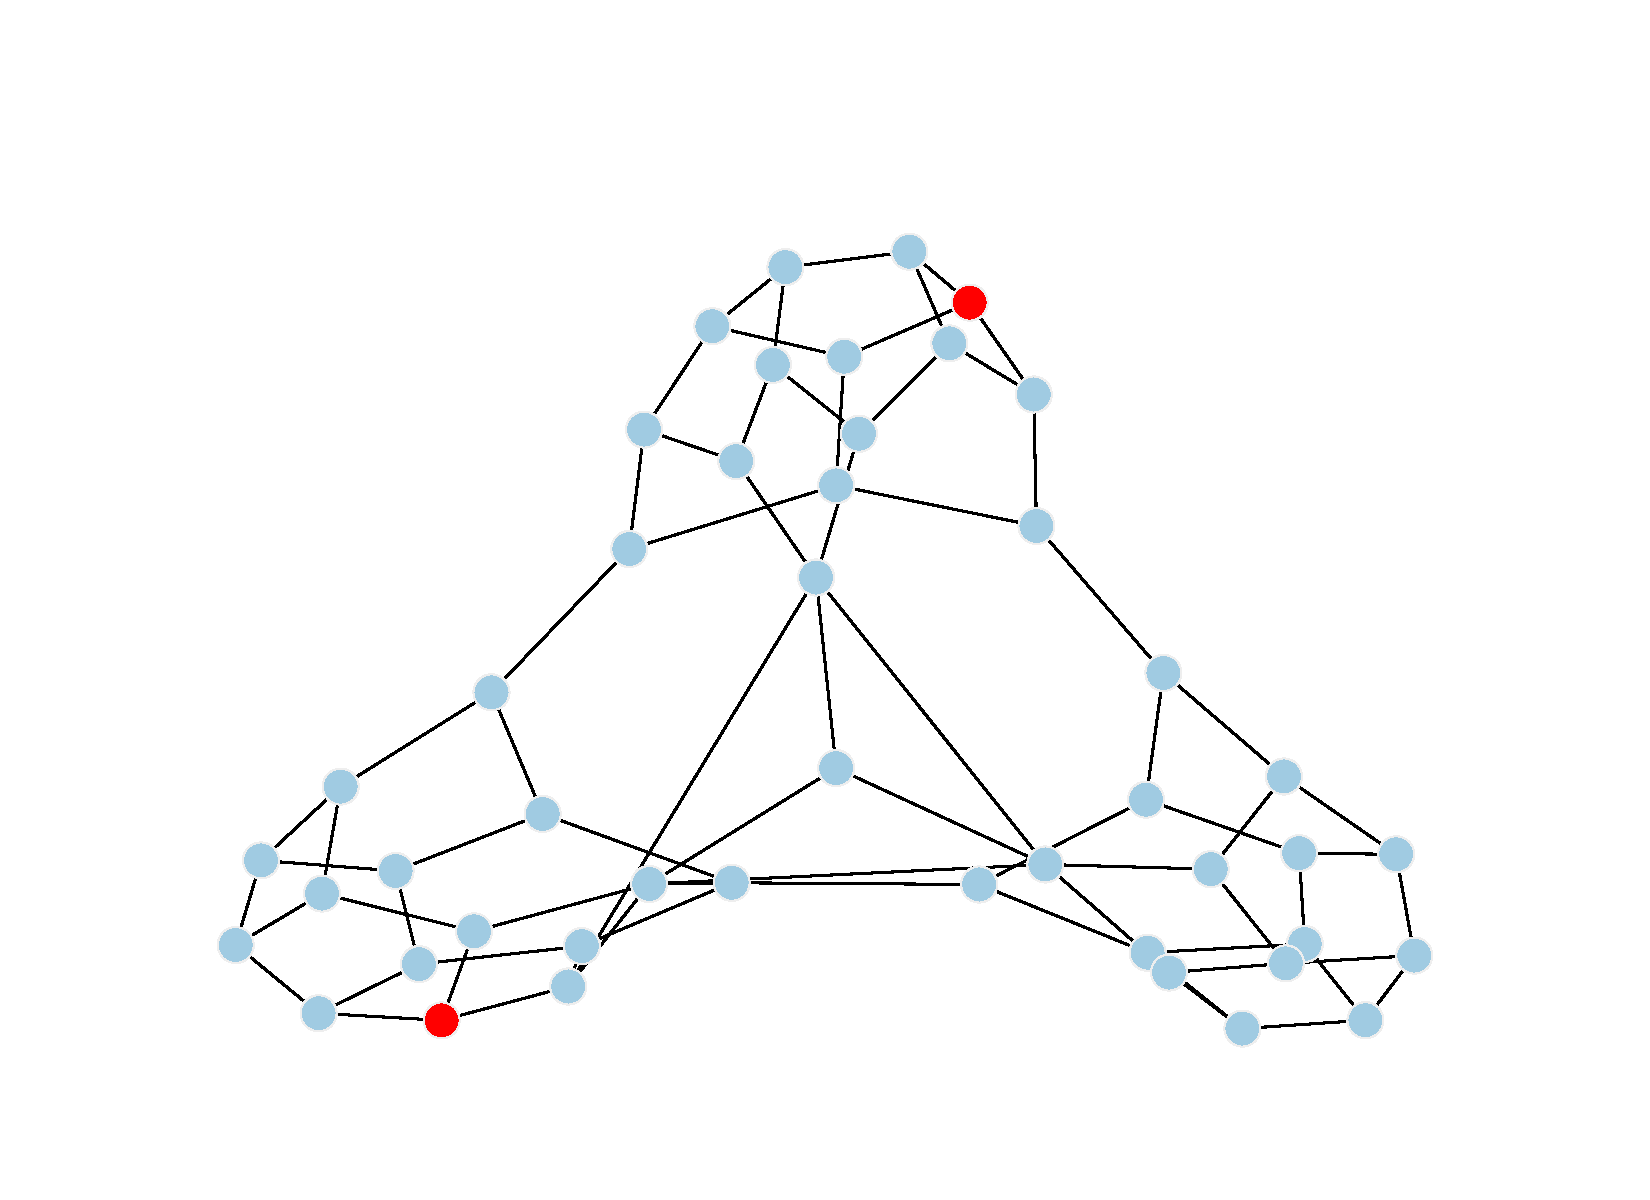
\includegraphics[scale=0.6] {images/graph_space.pdf}
	\label{fig:graph_space}
}
\caption[A graph representing the space search problem}
\label{fig:subfigureExample}
\end{figure}



\newpage
\setcounter{secnumdepth}{1}
\section{Behavior analysis of Bush-Mosteller lineal and incremental learning algorithms}

\subsection{The Linear BM model}
$$f_{ij}(k+1) =α f_{ij}(k)  + (1-\alpha) \beta (k)$$ where $0 \leq \alpha \leq 1$  is the learning ratio and $\beta$(k) stands for the reward function associated with  the current  $k$-th exploration such that $\alpha$(k)=1 for a reward.


\subsubsection{Binary}

\begin{figure}[ht]
\centering
\subfigure[Fitness evolution]{
	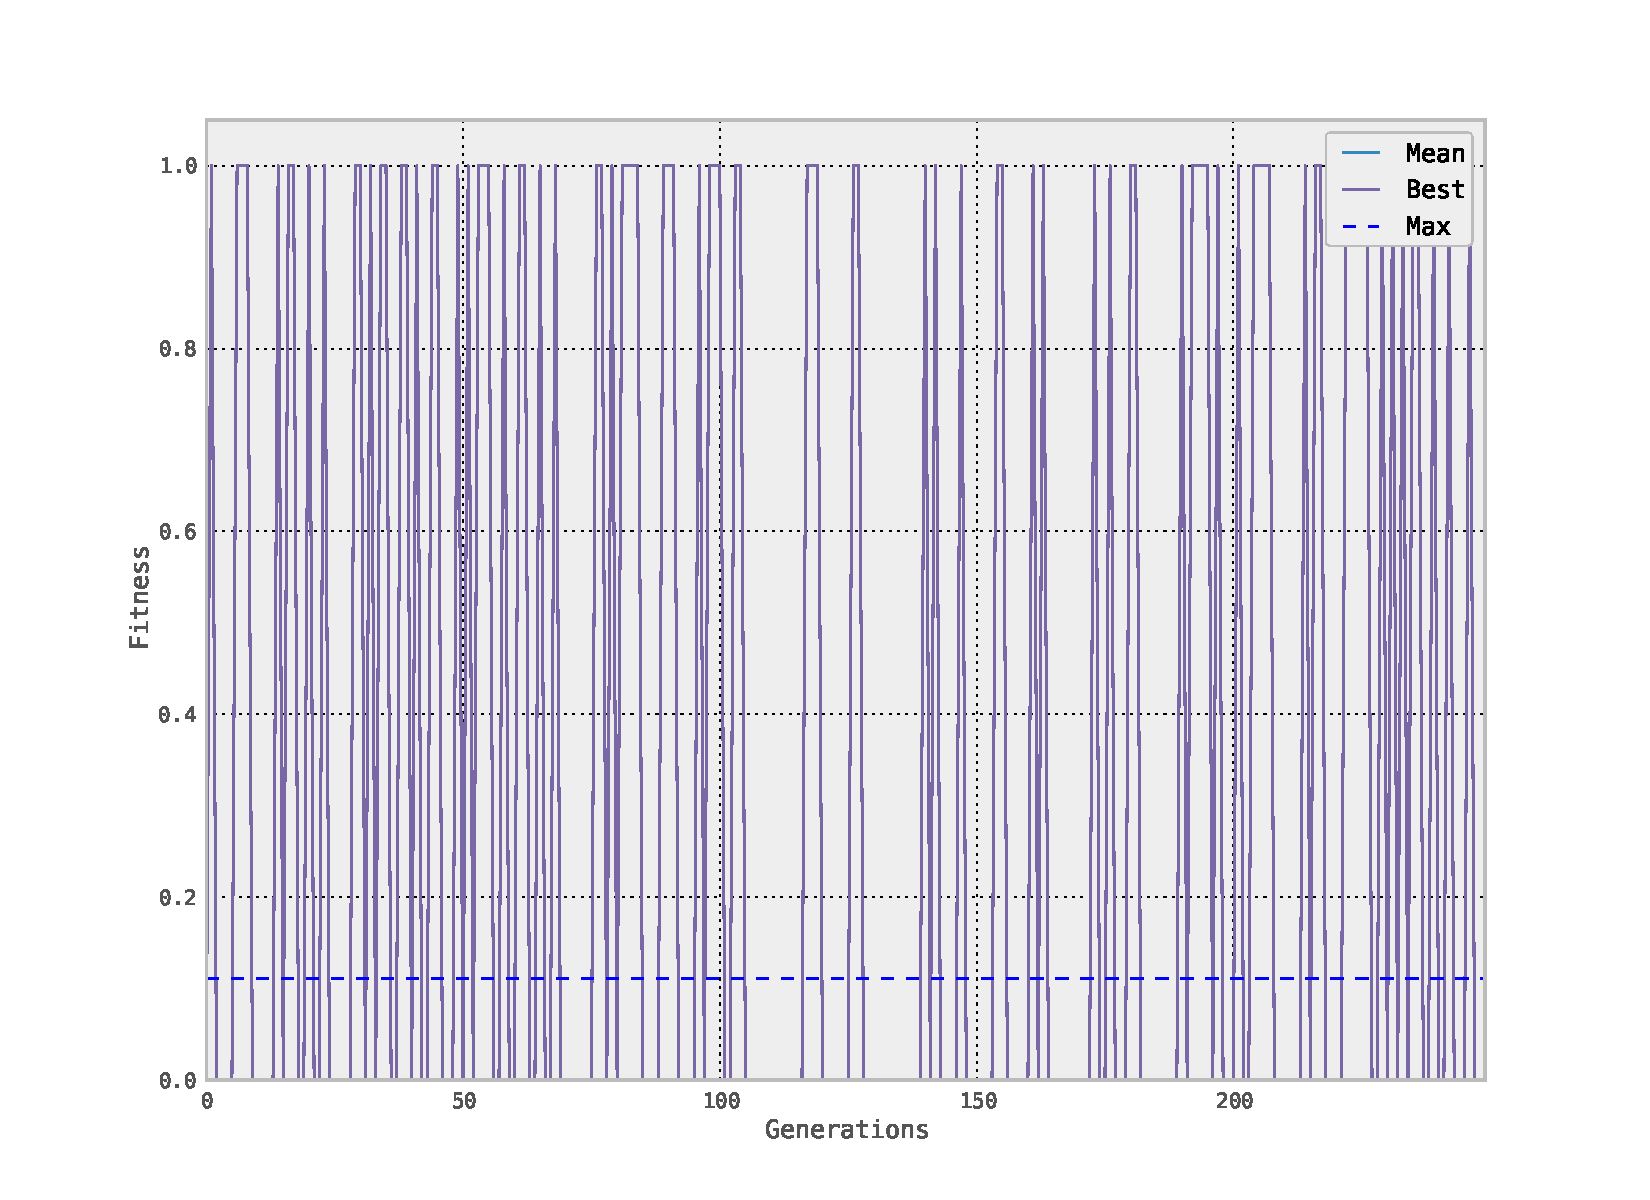
\includegraphics[scale =0.4] {images/section1/fitness_bush_mosteller_update_BinaryAnt.pdf}
	\label{fig:subfig11}
}
\subfigure[Pheromones per edge]{
	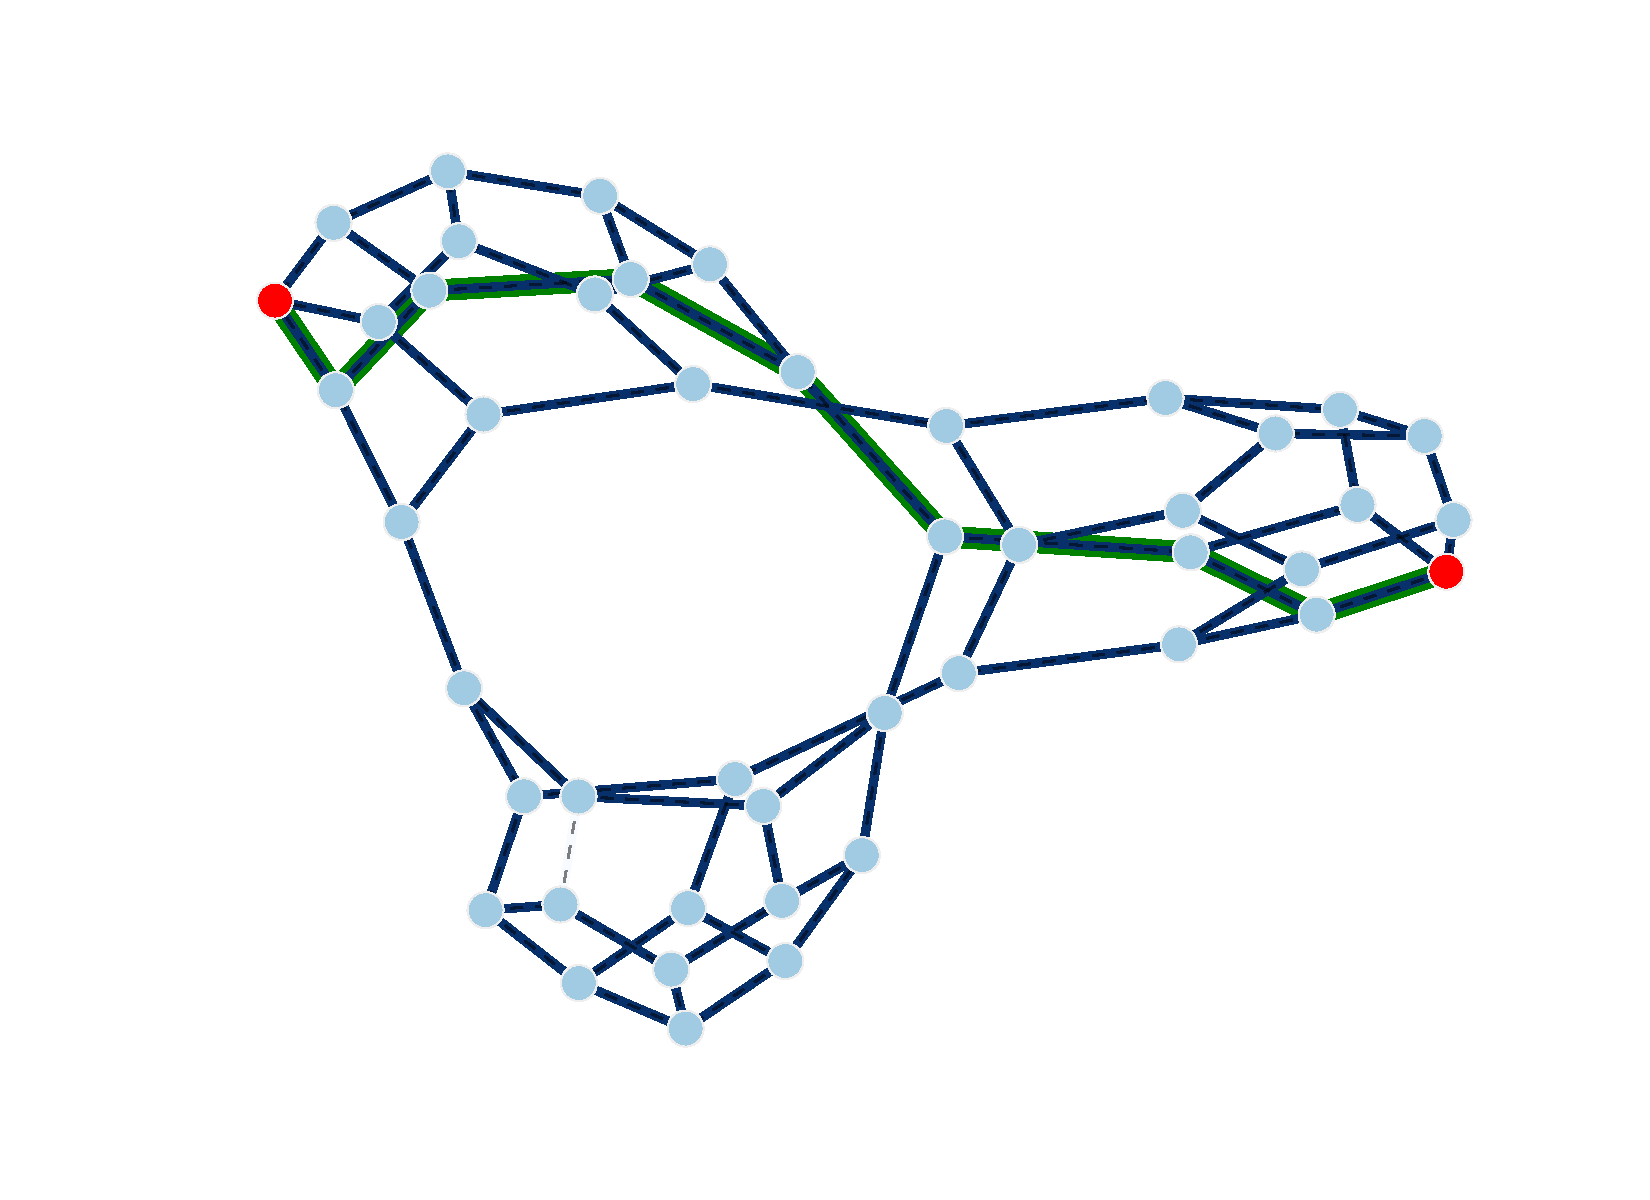
\includegraphics[scale =0.4] {images/section1/pheromones_bush_mosteller_update_BinaryAnt.pdf}
	\label{fig:subfig12}
}
%\caption[Optional caption for list of figures]{Caption of subfigures \subref{fig:subfig1}, \subref{fig:subfig2}}
\label{fig:fig1}
\end{figure}

\newpage
\subsubsection{Proportional}

\begin{figure}[ht]
\centering
\subfigure[Fitness evolution]{
	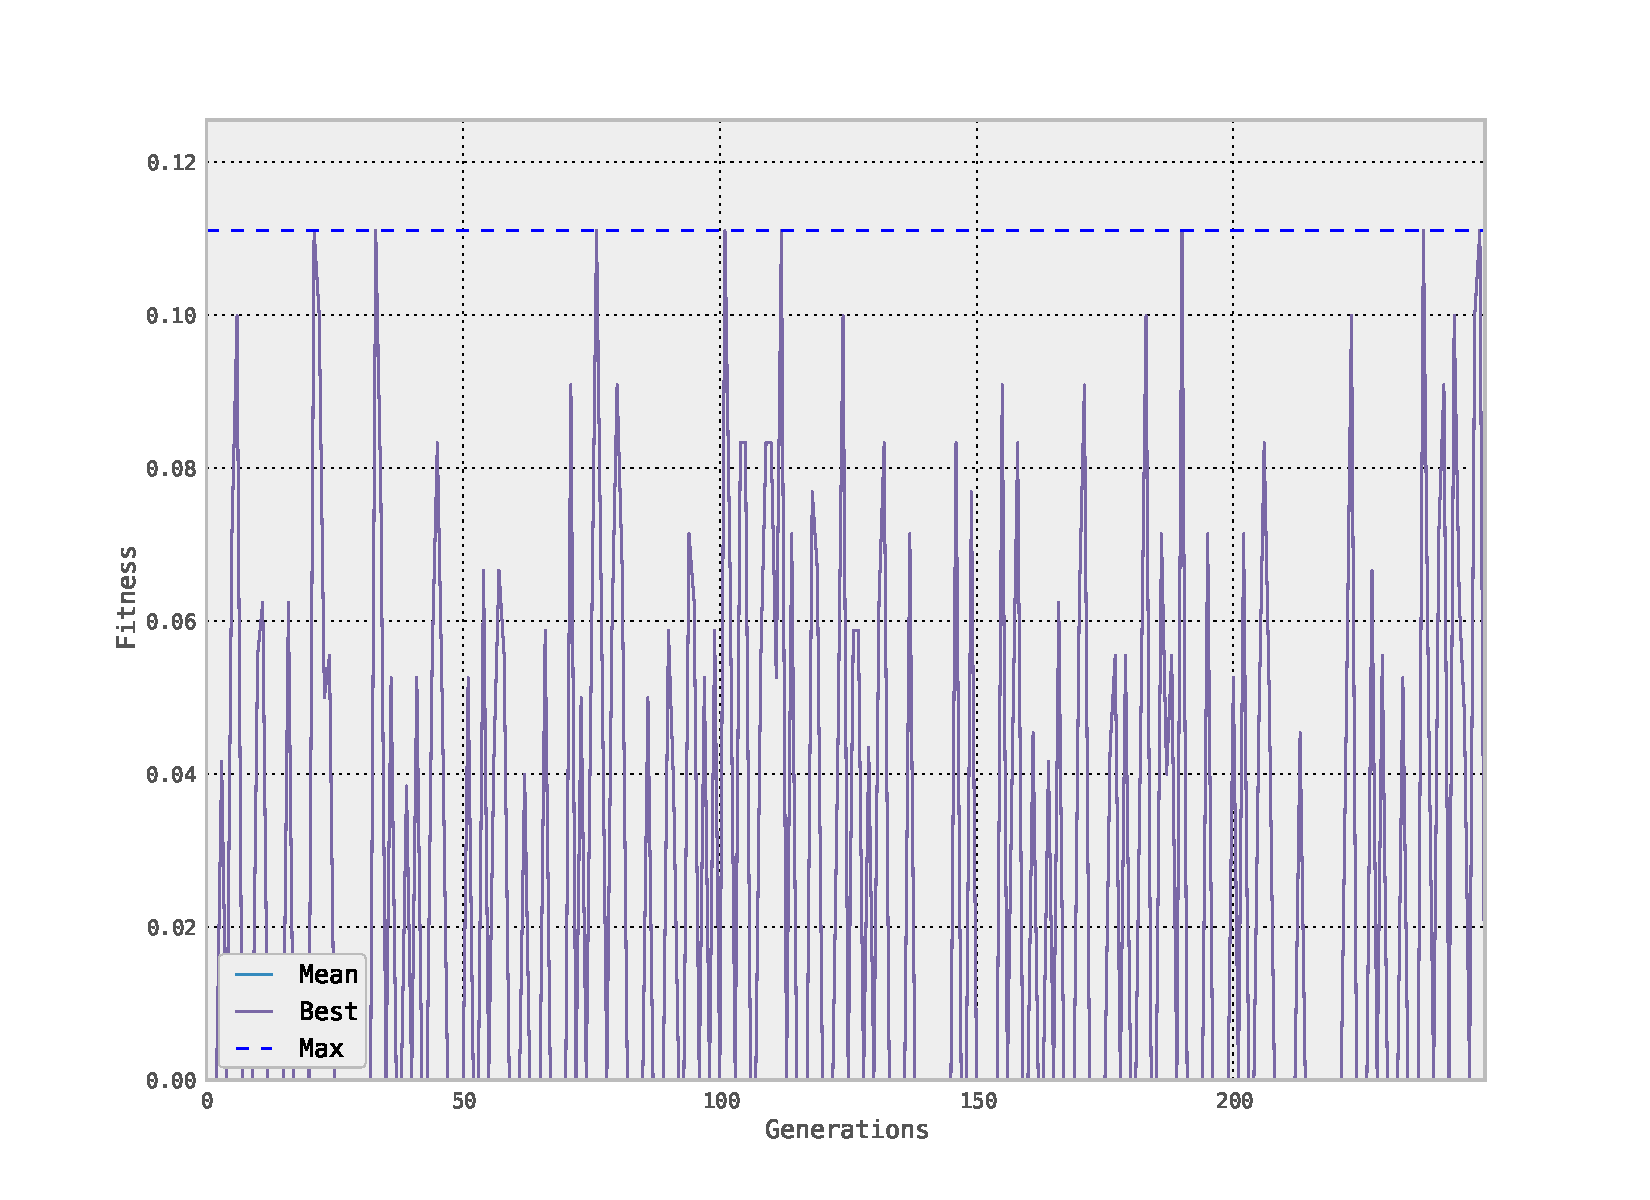
\includegraphics[scale =0.4] {images/section1/fitness_bush_mosteller_update_ProportionalAnt.pdf}
	\label{fig:subfig11}
}
\subfigure[Pheromones per edge]{
	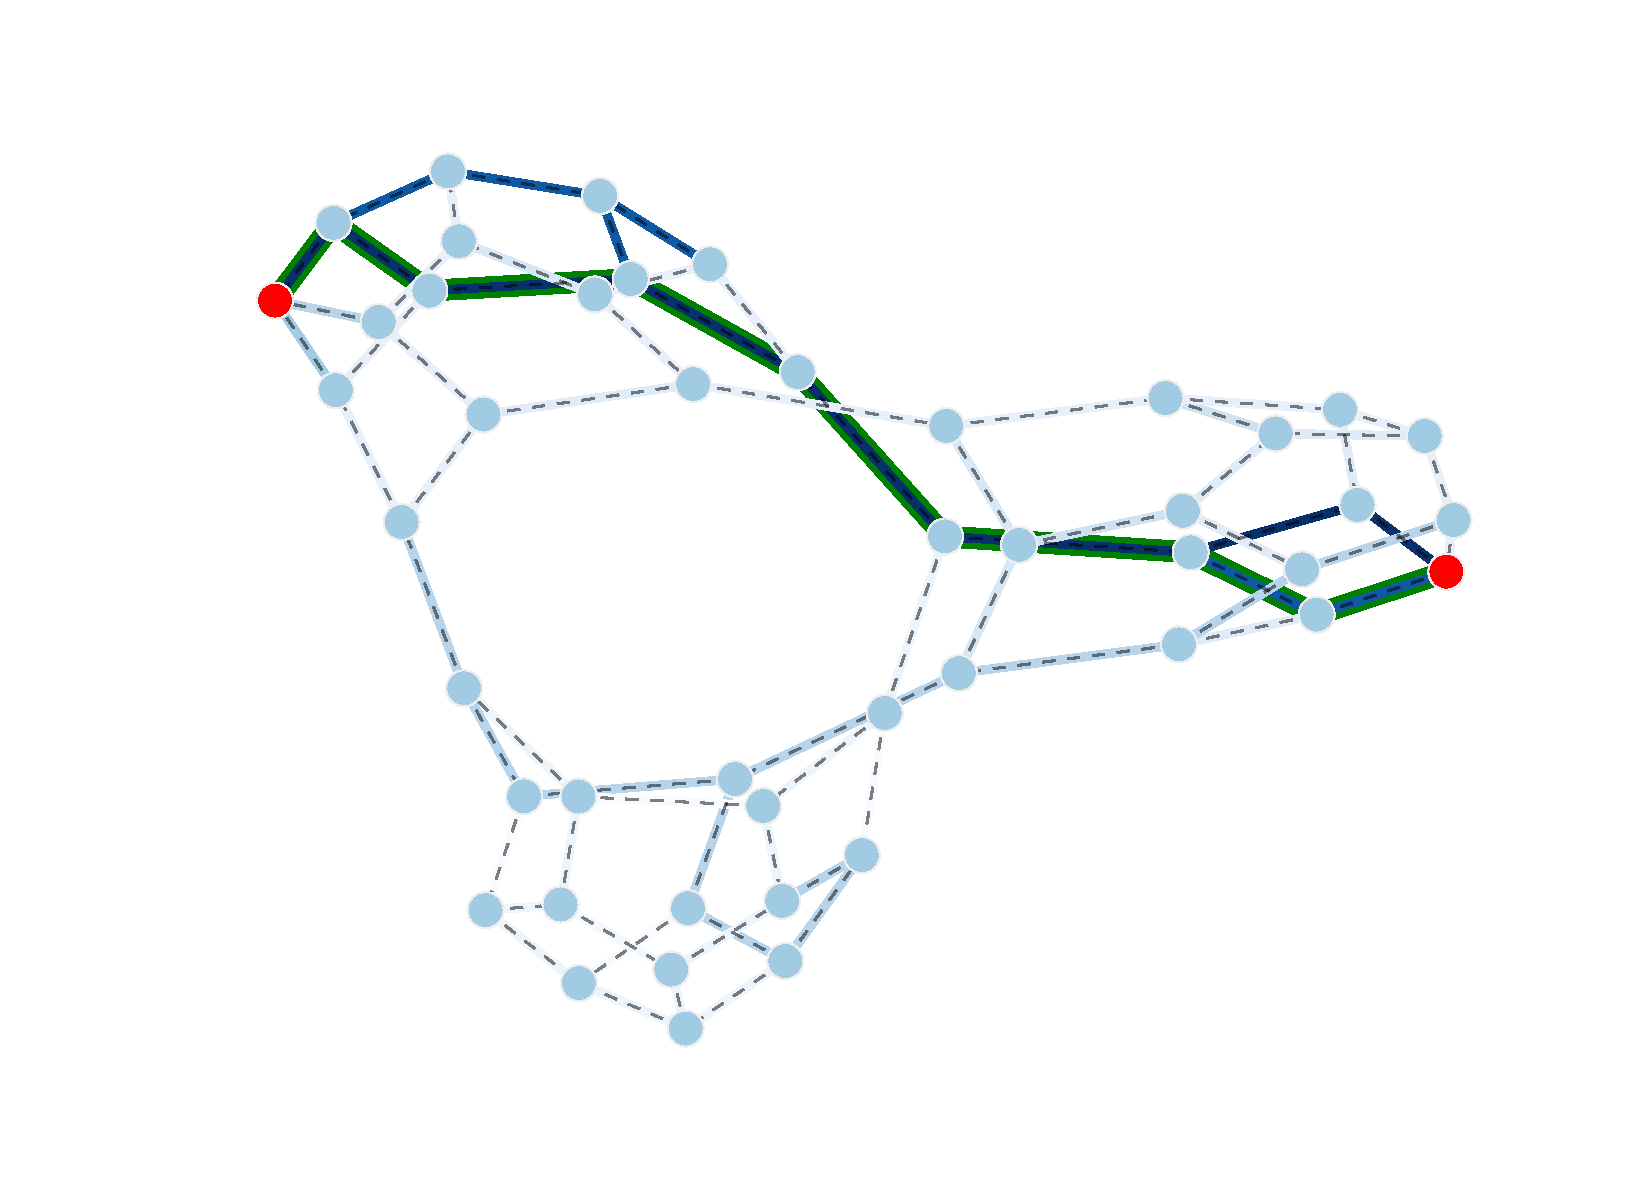
\includegraphics[scale =0.4] {images/section1/pheromones_bush_mosteller_update_ProportionalAnt.pdf}
	\label{fig:subfig12}
}
%\caption[Optional caption for list of figures]{Caption of subfigures \subref{fig:subfig1}, \subref{fig:subfig2}}
\label{fig:fig1}
\end{figure}














\newpage
\subsection{The incremental learning algorithm}
$$f_{ij} (k+1)   = f_{ij} (k) + \delta \beta(k)$$
where $0 \leq \delta \leq 1$ is the increment  design parameter and the reward signal $\beta$(k) has the same interpretation than in the previous algorithm.

\subsubsection{Binary}

\begin{figure}[ht]
\centering
\subfigure[Fitness evolution]{
	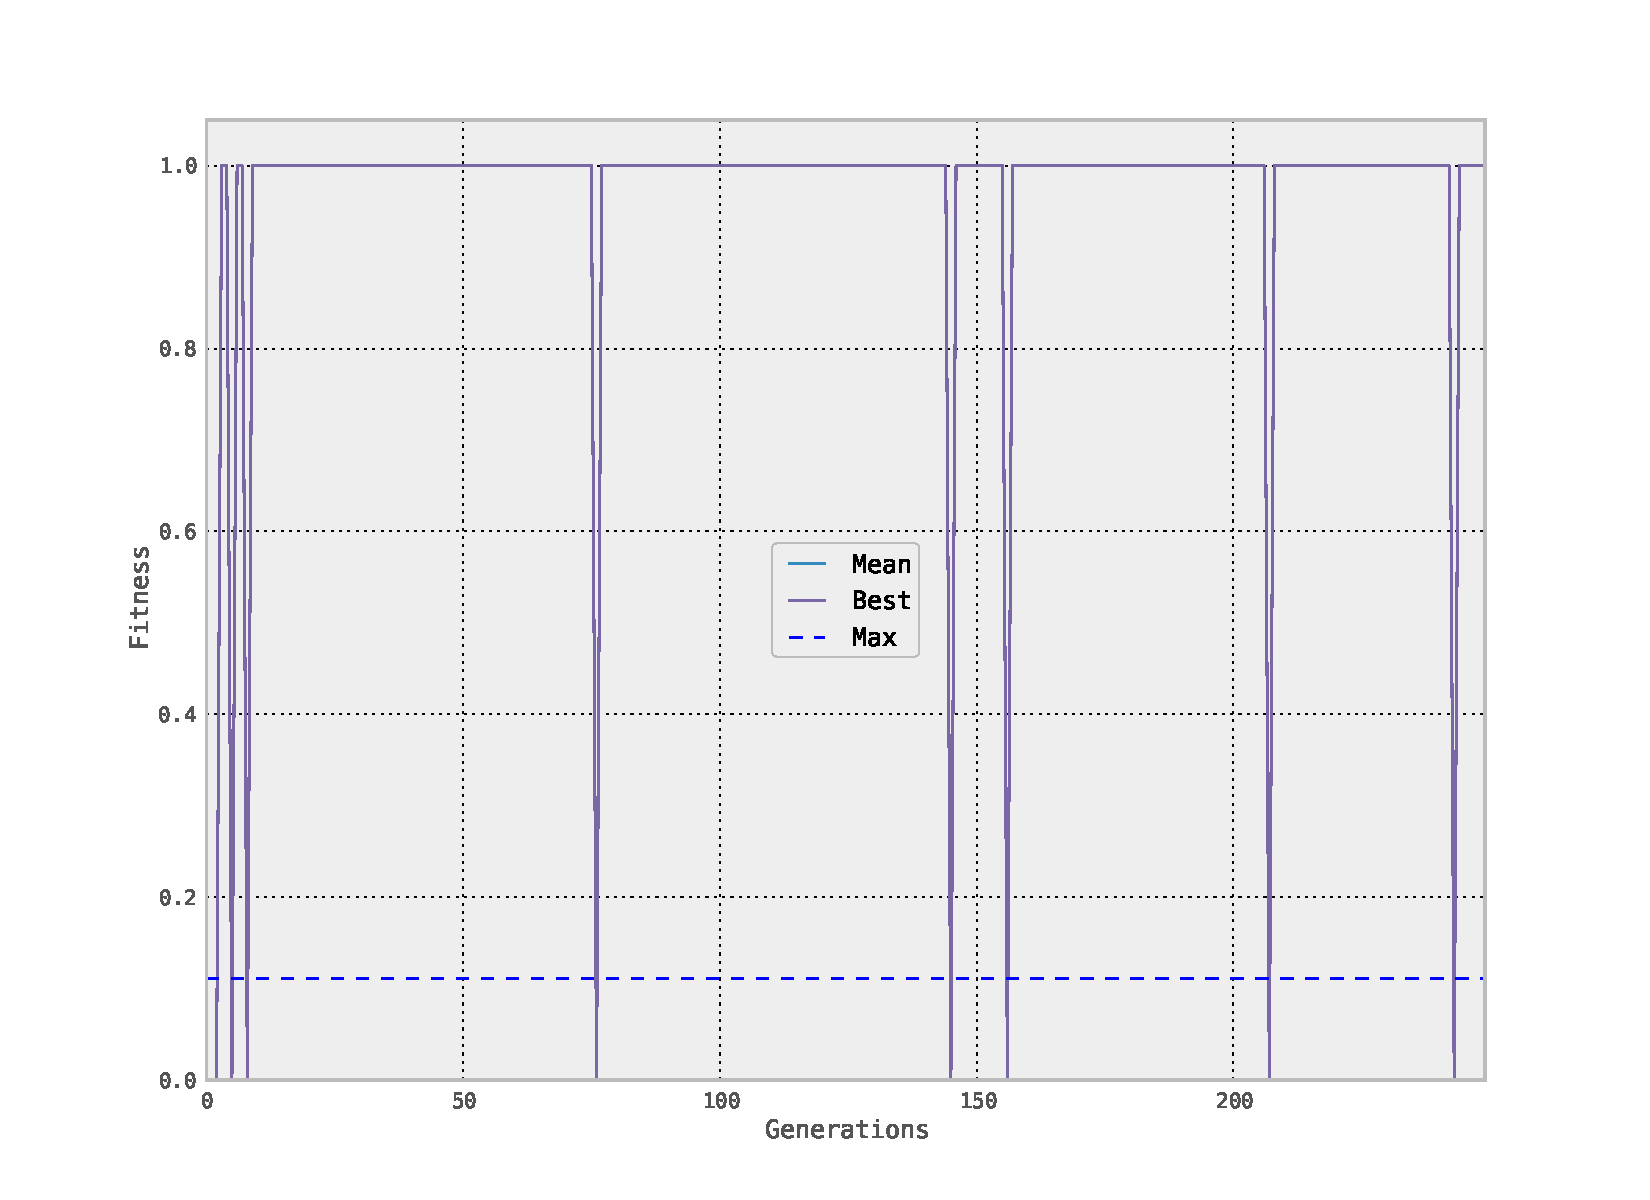
\includegraphics[scale =0.3] {images/section1/fitness_incremental_learning_update_BinaryAnt.pdf}
	\label{fig:subfig11}
}
\subfigure[Pheromones per edge]{
	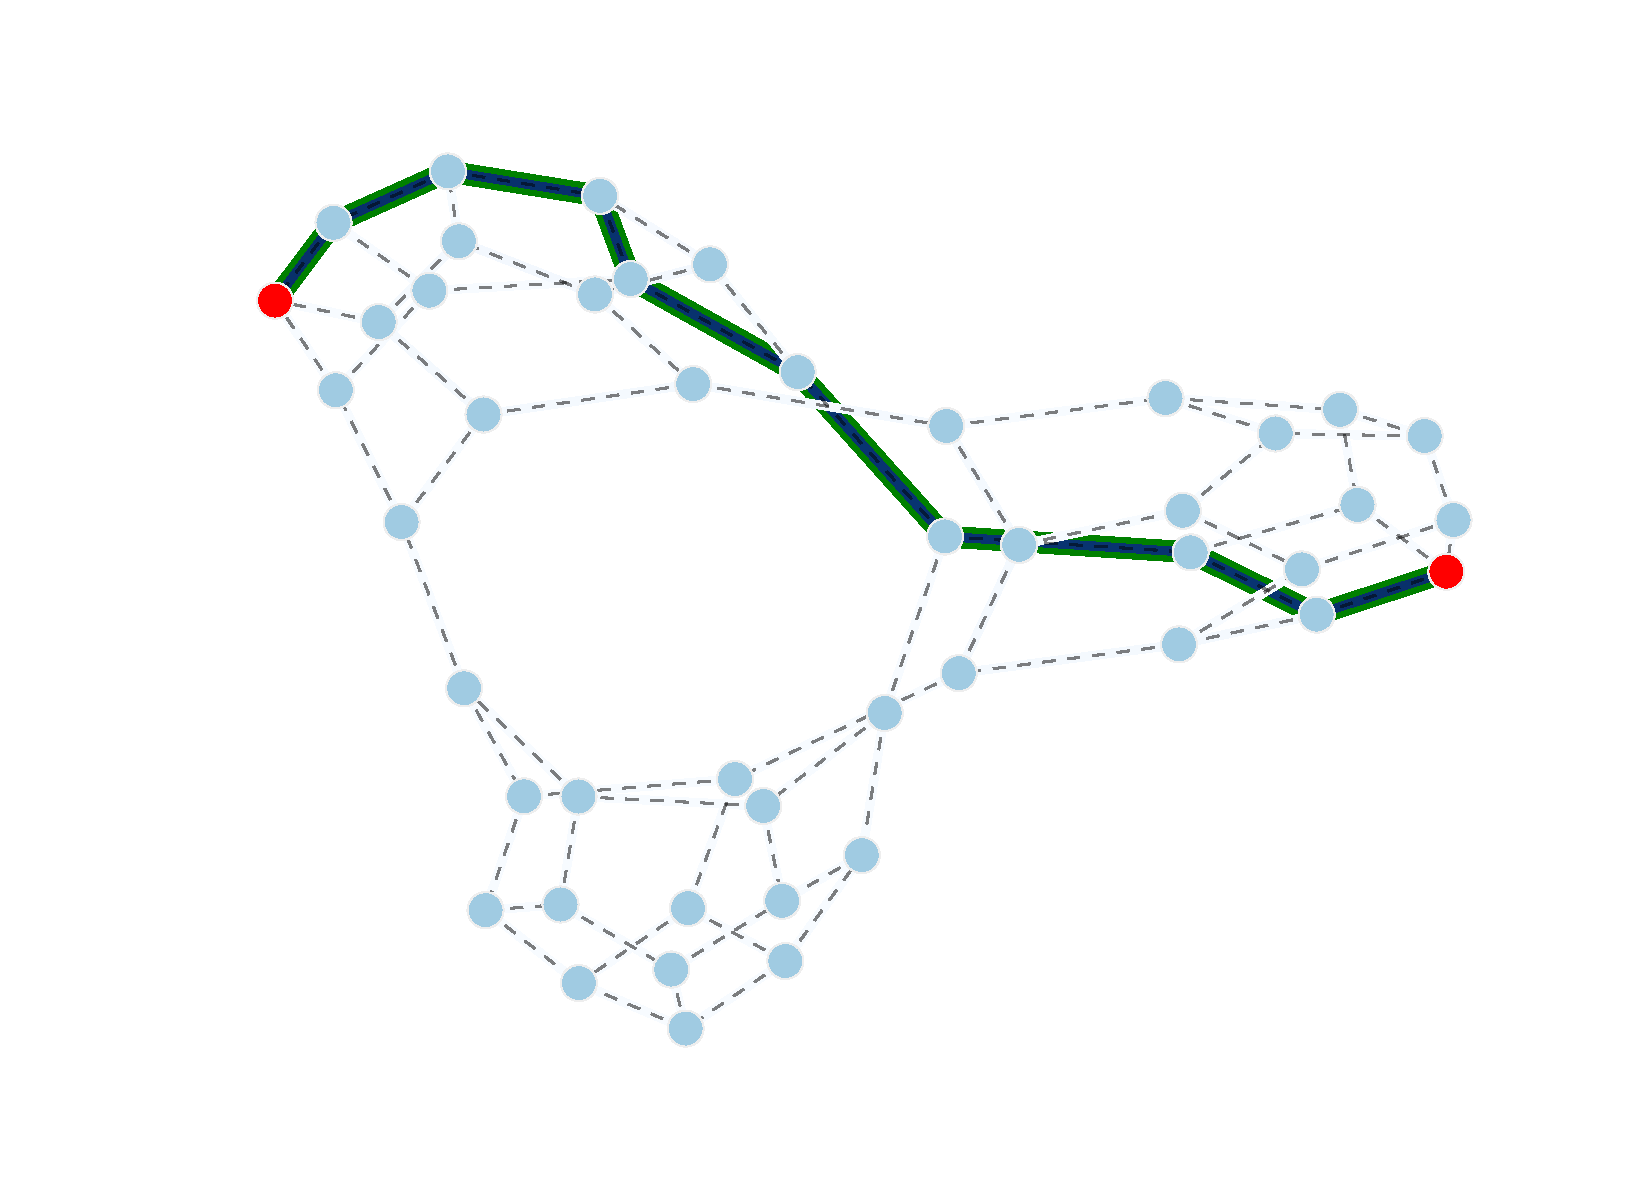
\includegraphics[scale =0.3] {images/section1/pheromones_incremental_learning_update_BinaryAnt.pdf}
	\label{fig:subfig12}
}
%\caption[Optional caption for list of figures]{Caption of subfigures \subref{fig:subfig1}, \subref{fig:subfig2}}
\label{fig:fig1}
\end{figure}

\newpage
\subsubsection{Proportional}

\begin{figure}[ht]
\centering
\subfigure[Fitness evolution]{
	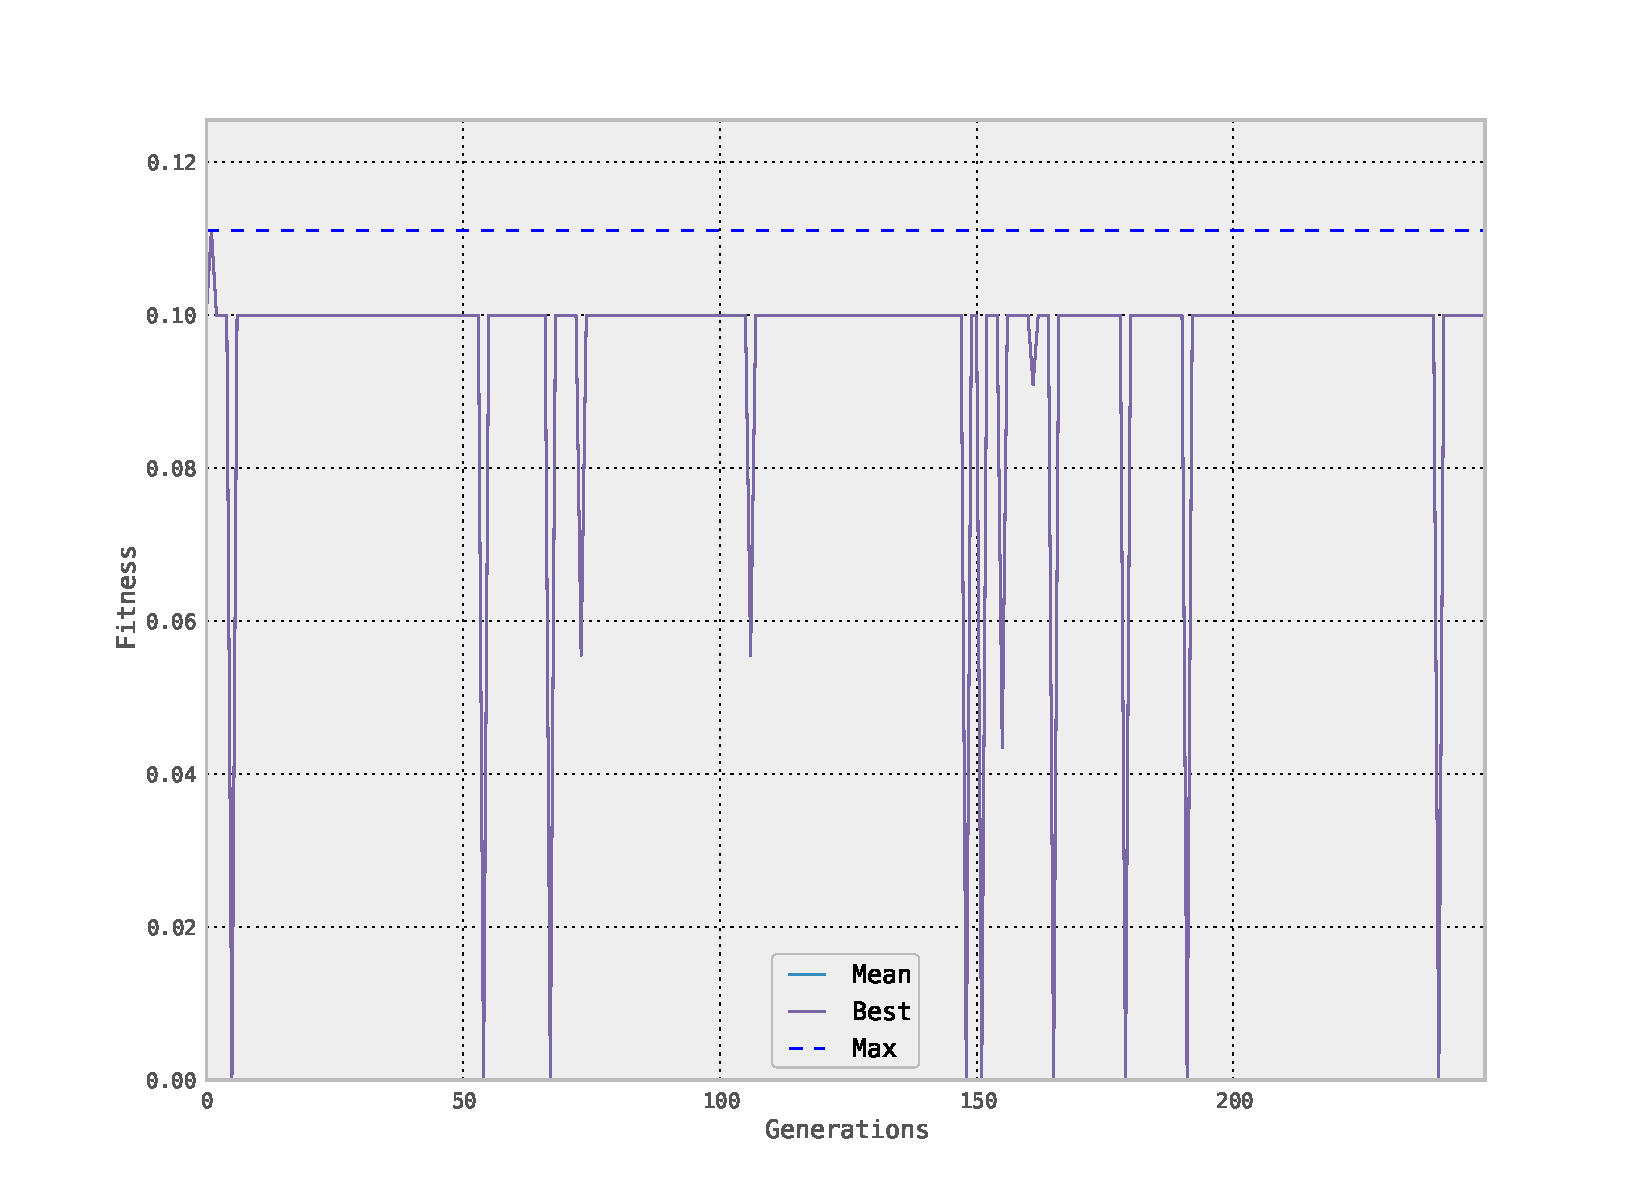
\includegraphics[scale =0.3] {images/section1/fitness_incremental_learning_update_ProportionalAnt.pdf}
	\label{fig:subfig11}
}
\subfigure[Pheromones per edge]{
	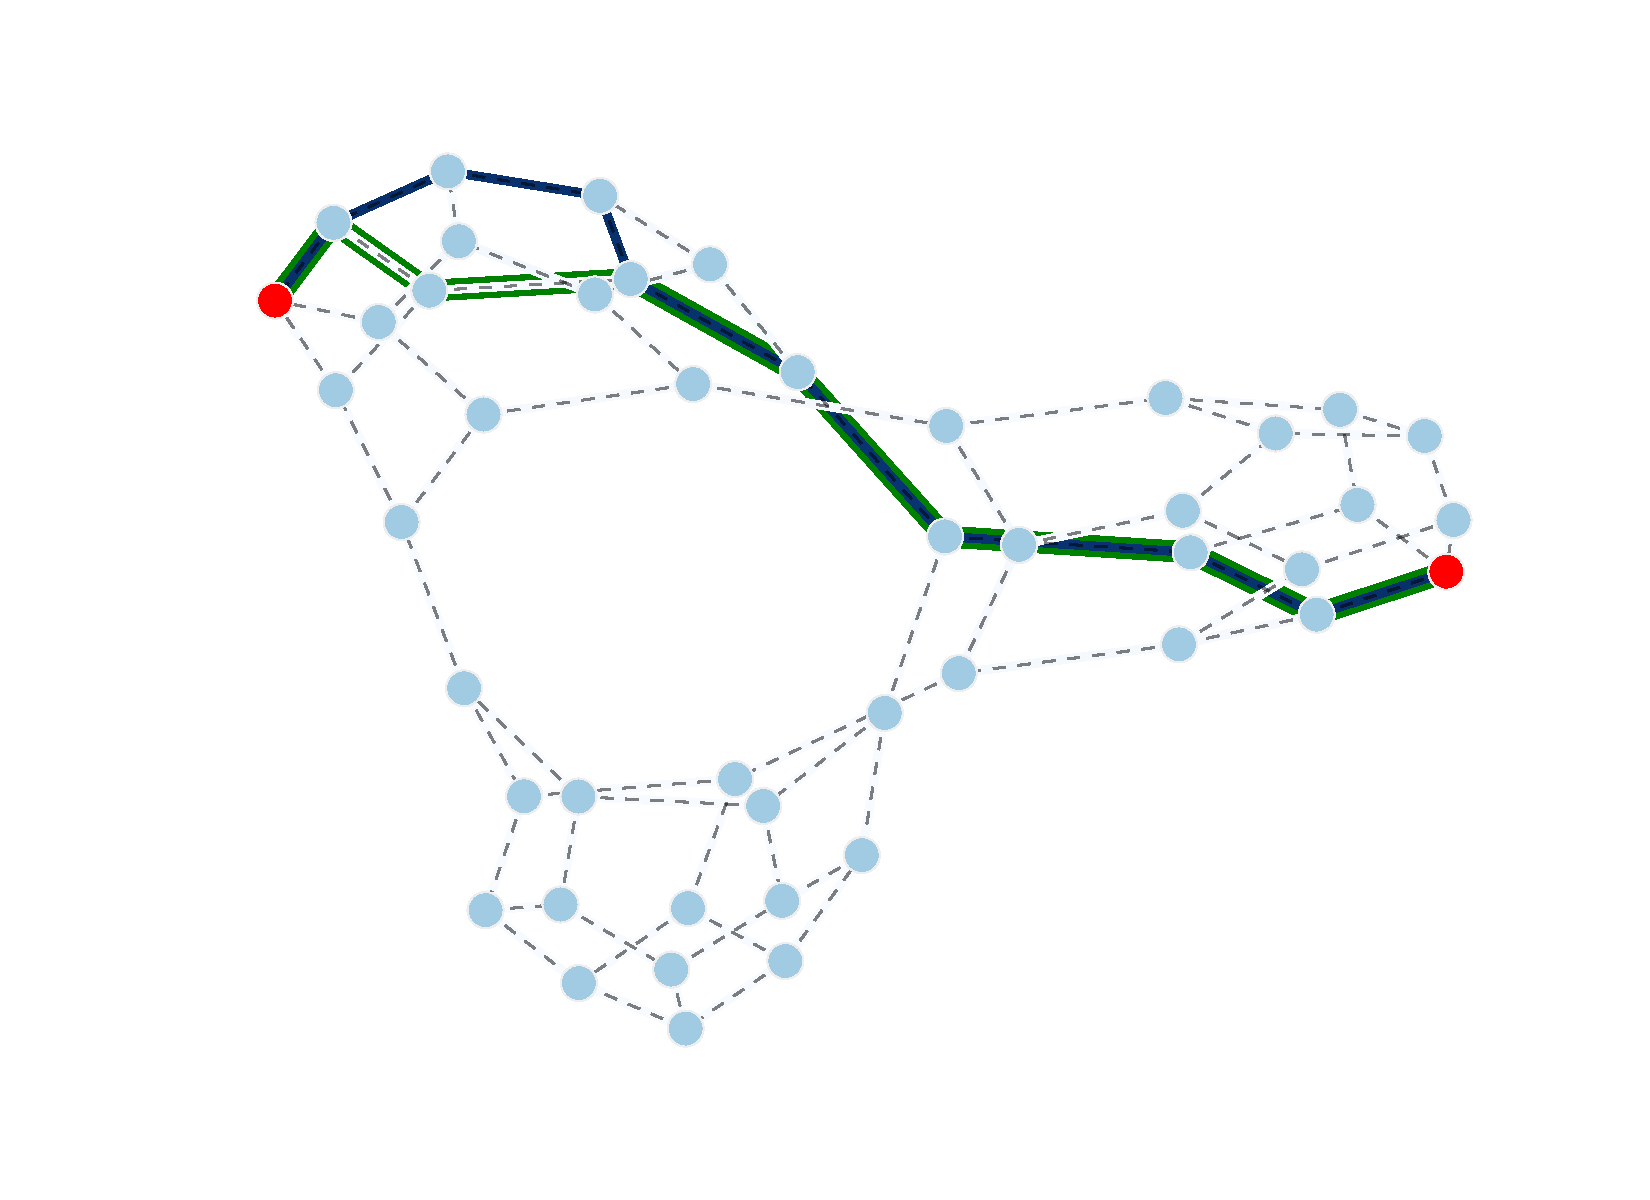
\includegraphics[scale =0.3] {images/section1/pheromones_incremental_learning_update_ProportionalAnt.pdf}
	\label{fig:subfig12}
}
%\caption[Optional caption for list of figures]{Caption of subfigures \subref{fig:subfig1}, \subref{fig:subfig2}}
\label{fig:fig1}
\end{figure}







\newpage
\subsection{Conclusions}
As the results shows, we can see that The Linear BM model + Binary, we perform a huge exploration reaching the best path randomly. With a The Linear BM model + Proportional the method is able to make a bias to the best one. The incremental learning algorithm works perfectly to reaching the optimal path.
\newpage
\section{Behavior analysis of collective exploration ant-like I \& II algorithms}


\subsubsection{Ant-like I, $k=5$}

\begin{figure}[ht]
\centering
\subfigure[Fitness evolution]{
	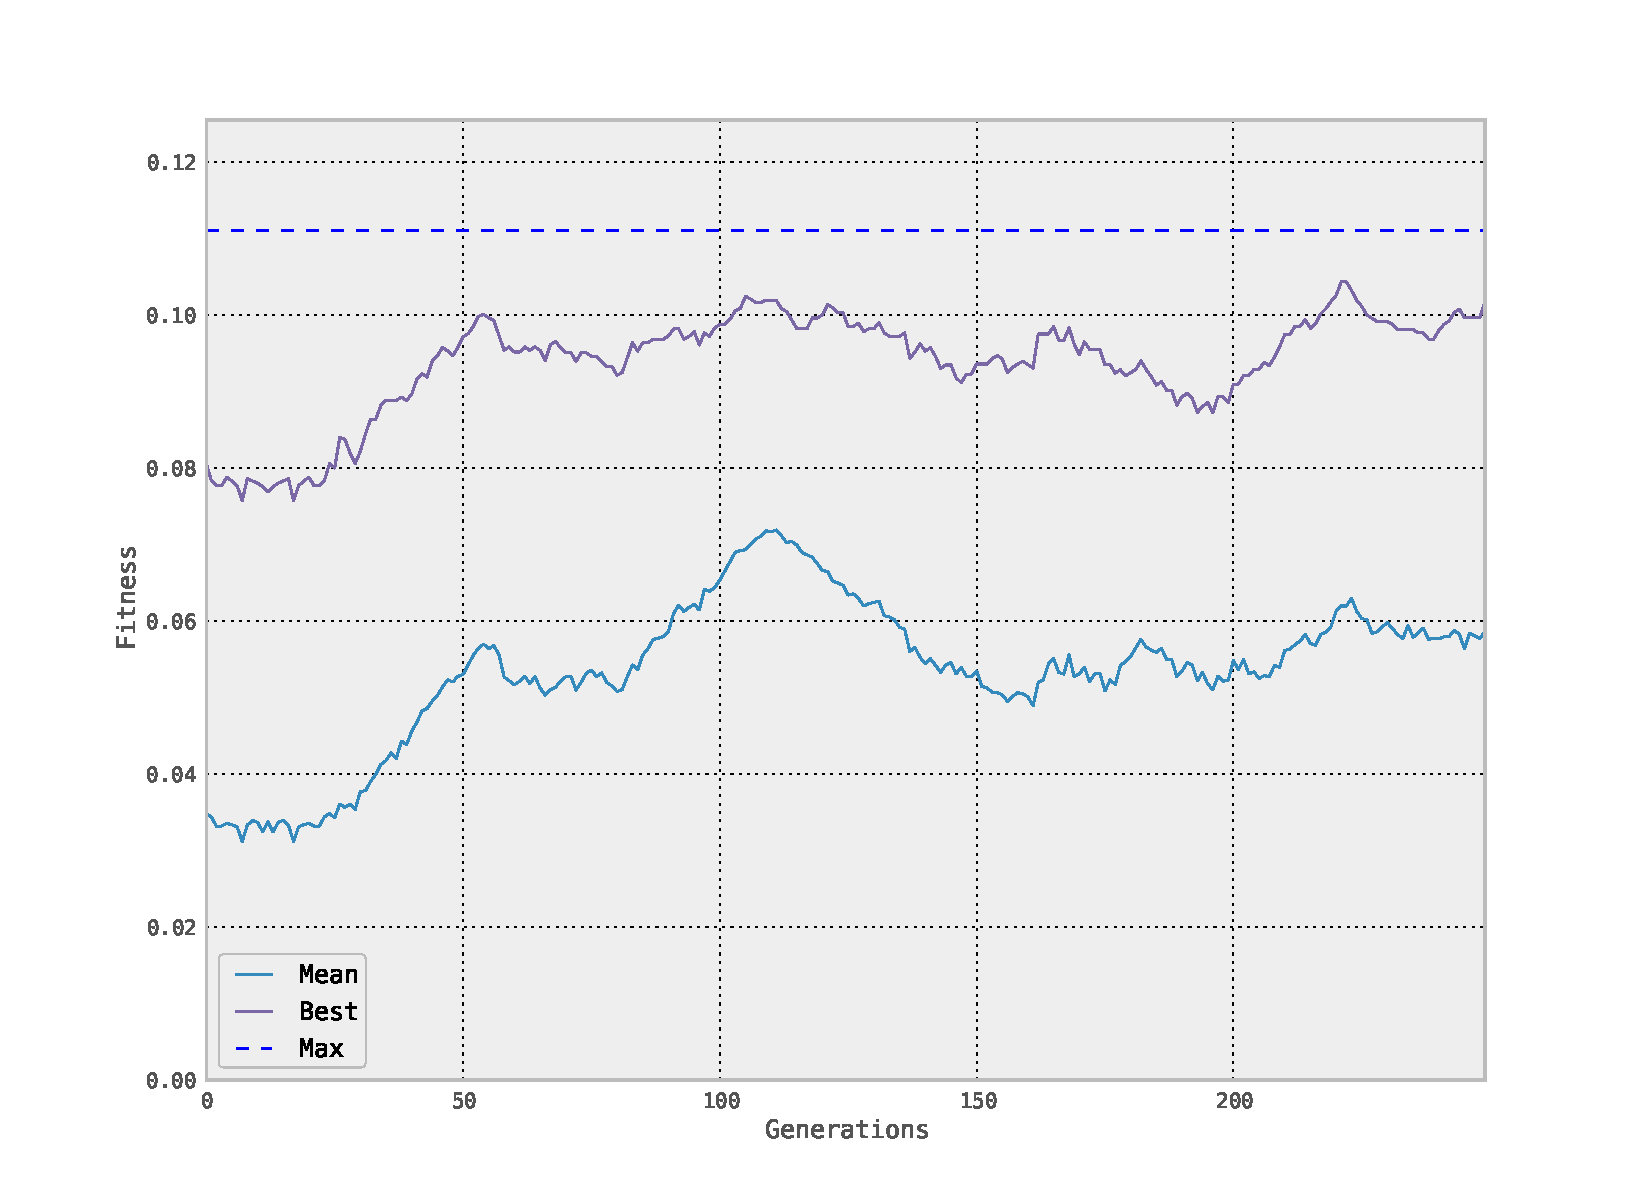
\includegraphics[scale =0.4] {images/section2/experimenta/fitness_5.pdf}
	\label{fig:subfig11}
}
\subfigure[Pheromones per edge]{
	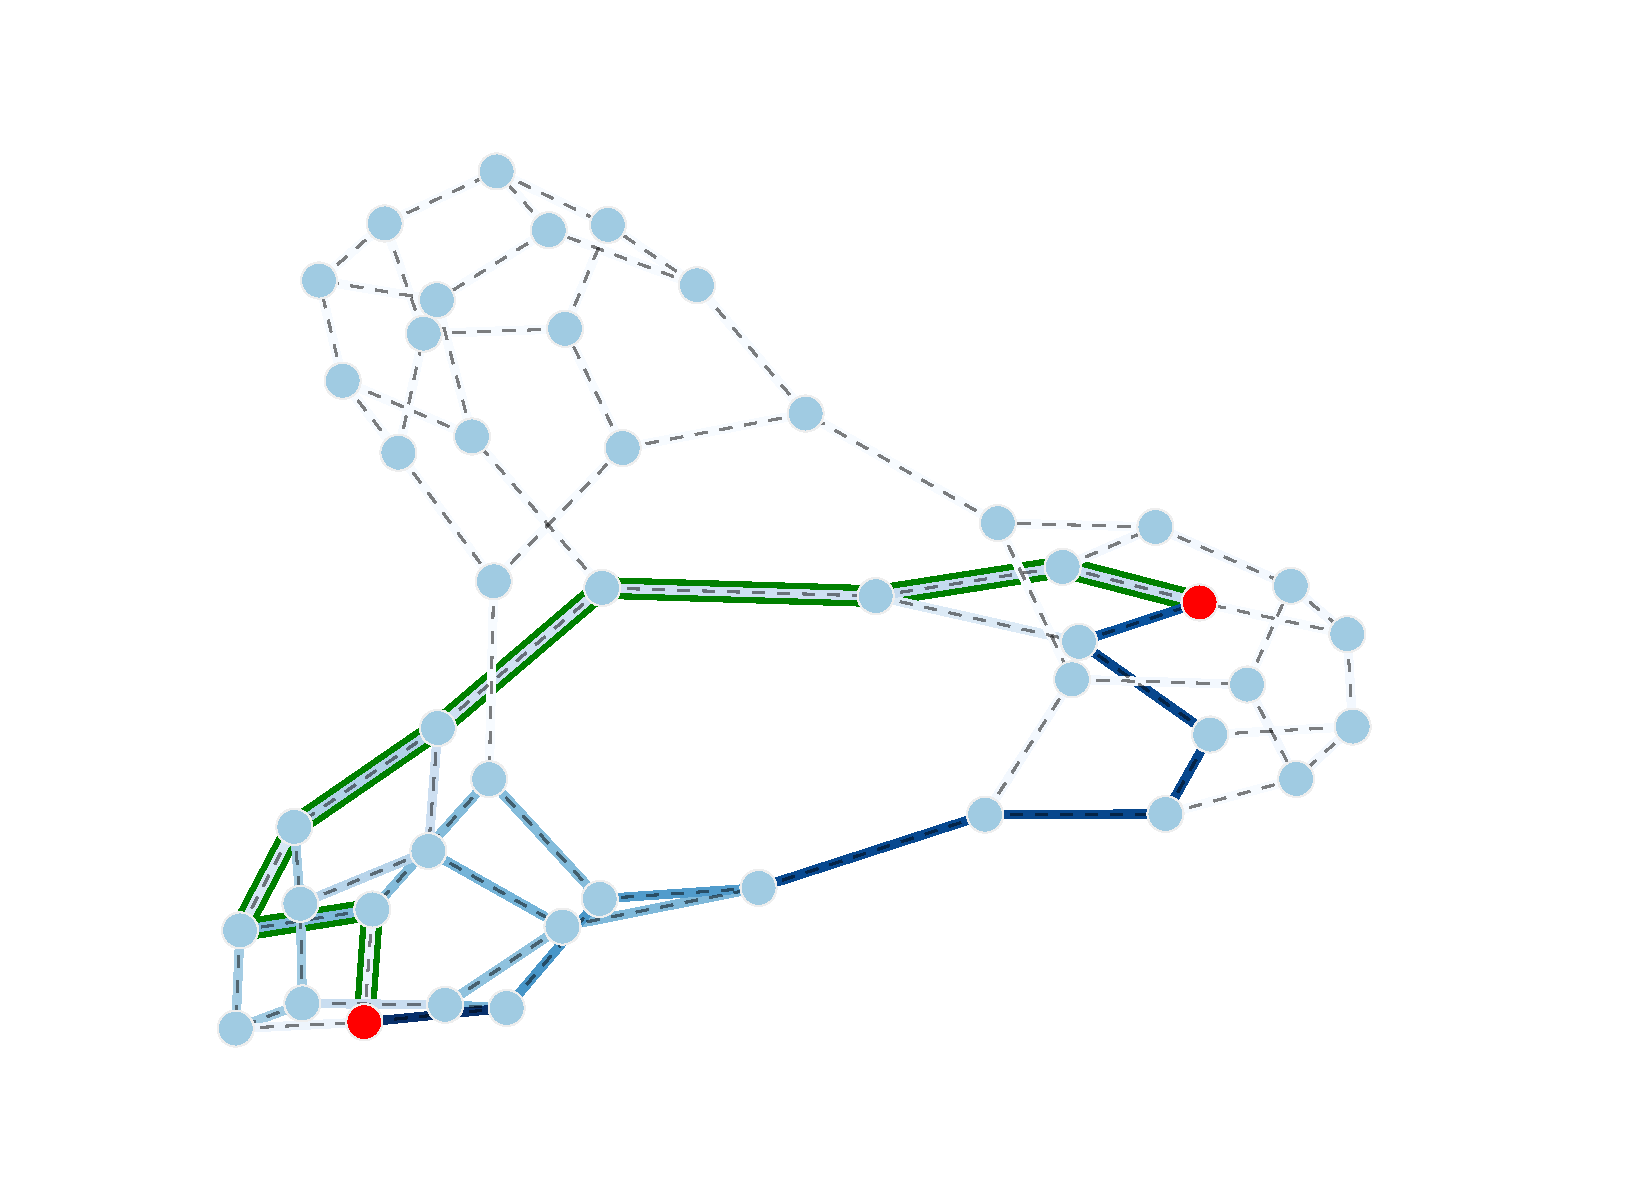
\includegraphics[scale =0.4] {images/section2/experimenta/pheromones_5_.pdf}
	\label{fig:subfig12}
}
%\caption[Optional caption for list of figures]{Caption of subfigures \subref{fig:subfig1}, \subref{fig:subfig2}}
\label{fig:fig1}
\end{figure}


\newpage
\subsubsection{Ant-like I, $k=10$}

\begin{figure}[ht]
\centering
\subfigure[Fitness evolution]{
	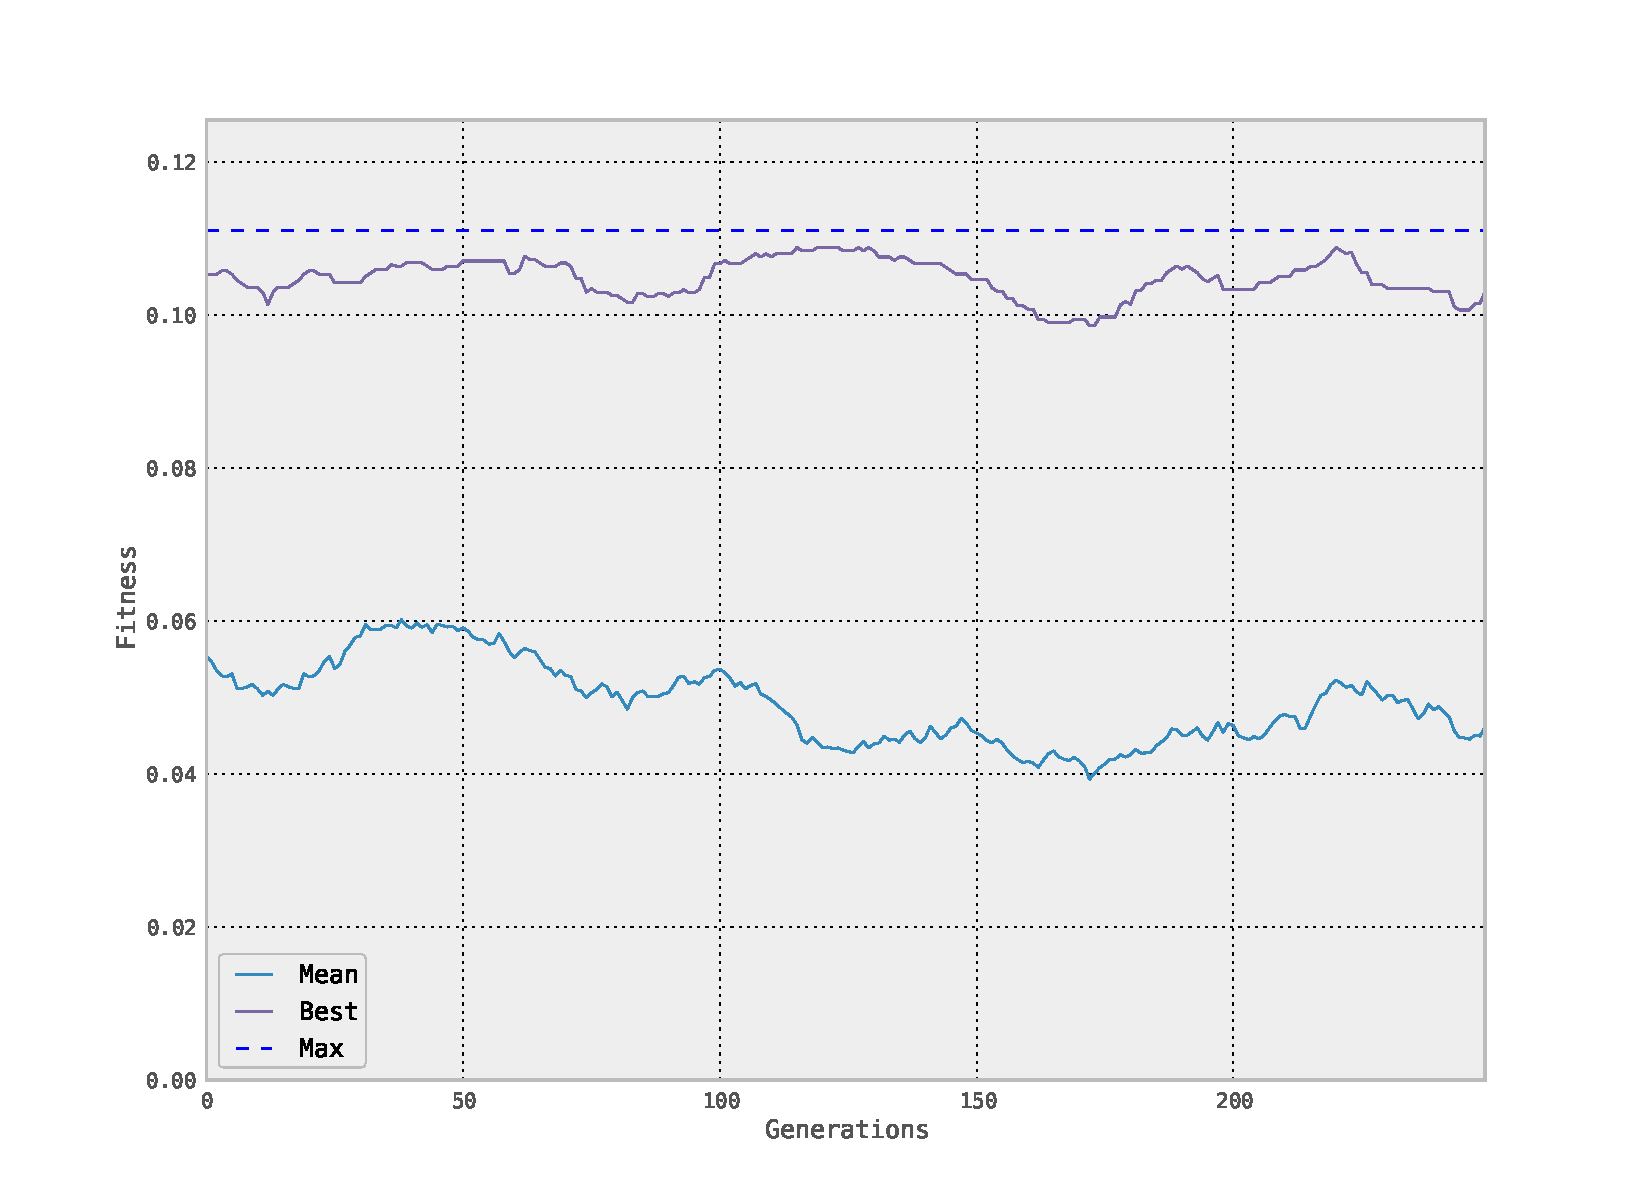
\includegraphics[scale =0.4] {images/section2/experimenta/fitness_10.pdf}
	\label{fig:subfig11}
}
\subfigure[Pheromones per edge]{
	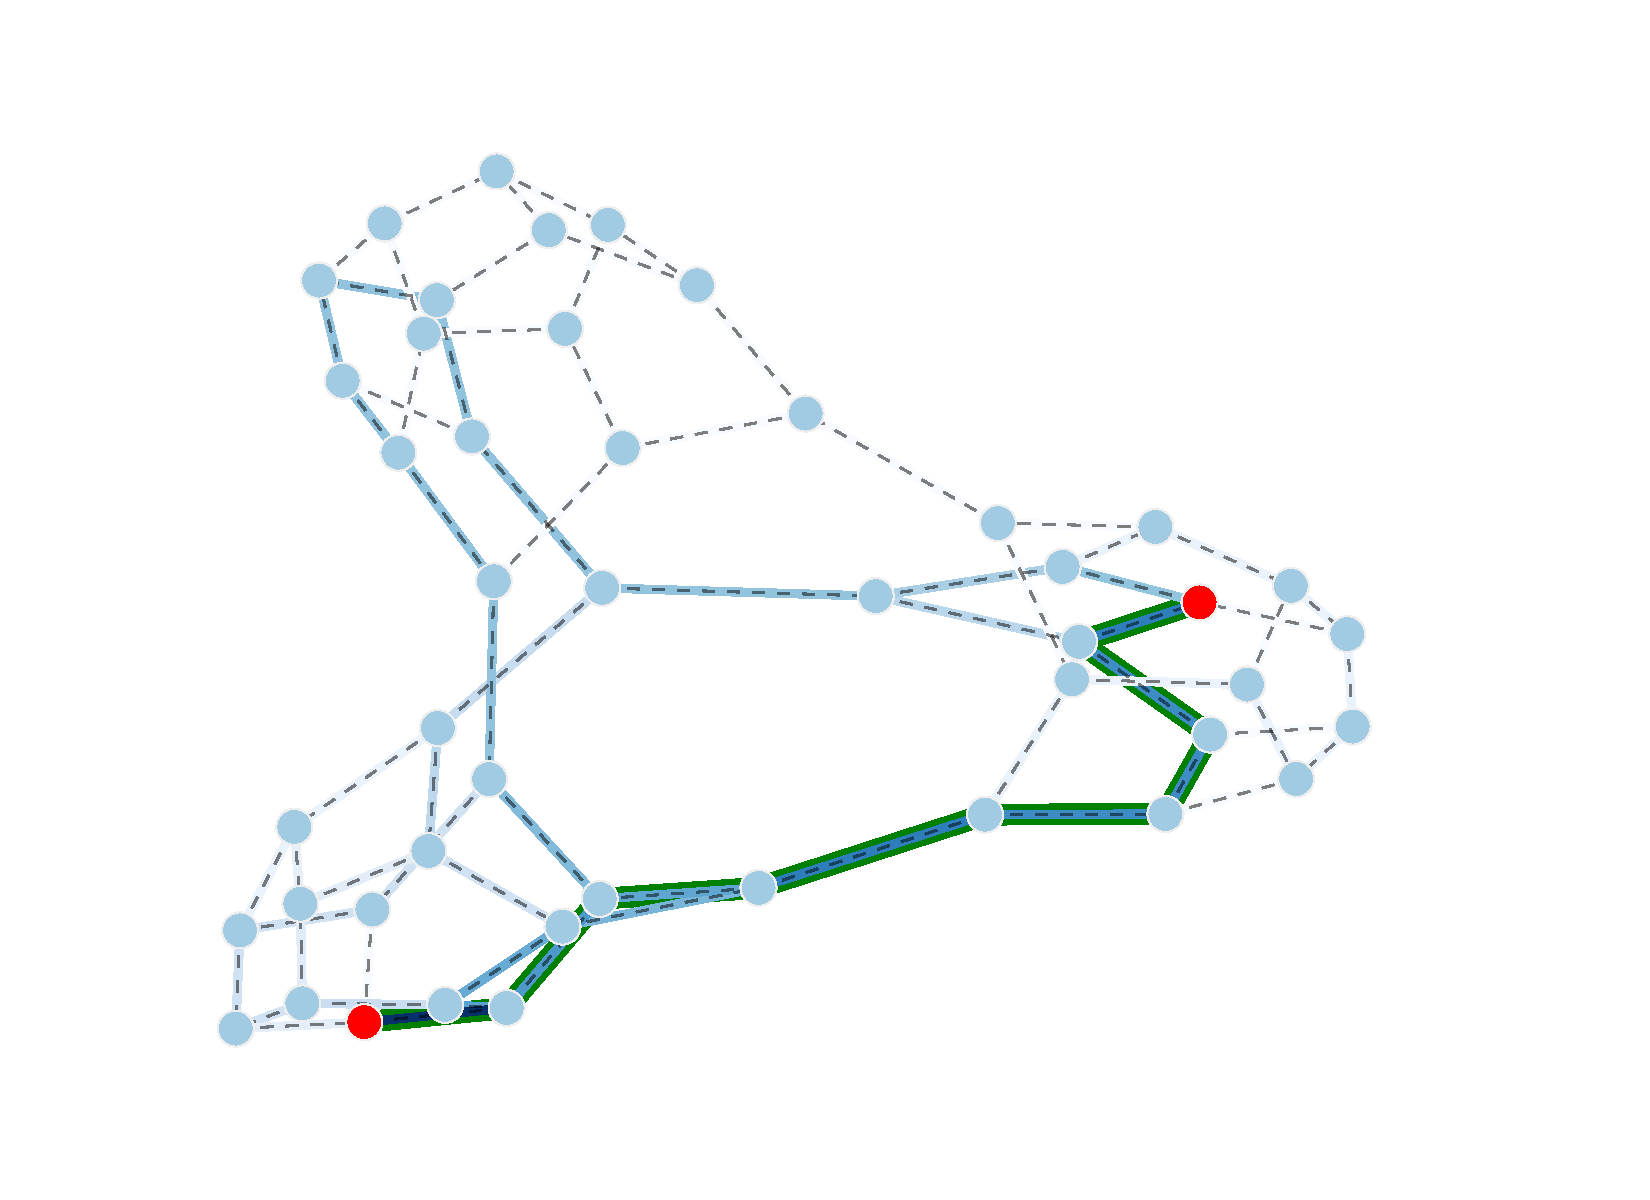
\includegraphics[scale =0.4] {images/section2/experimenta/pheromones_10_.pdf}
	\label{fig:subfig12}
}
%\caption[Optional caption for list of figures]{Caption of subfigures \subref{fig:subfig1}, \subref{fig:subfig2}}
\label{fig:fig1}
\end{figure}


\newpage
\subsubsection{Ant-like I, $k=15$}

\begin{figure}[ht]
\centering
\subfigure[Fitness evolution]{
	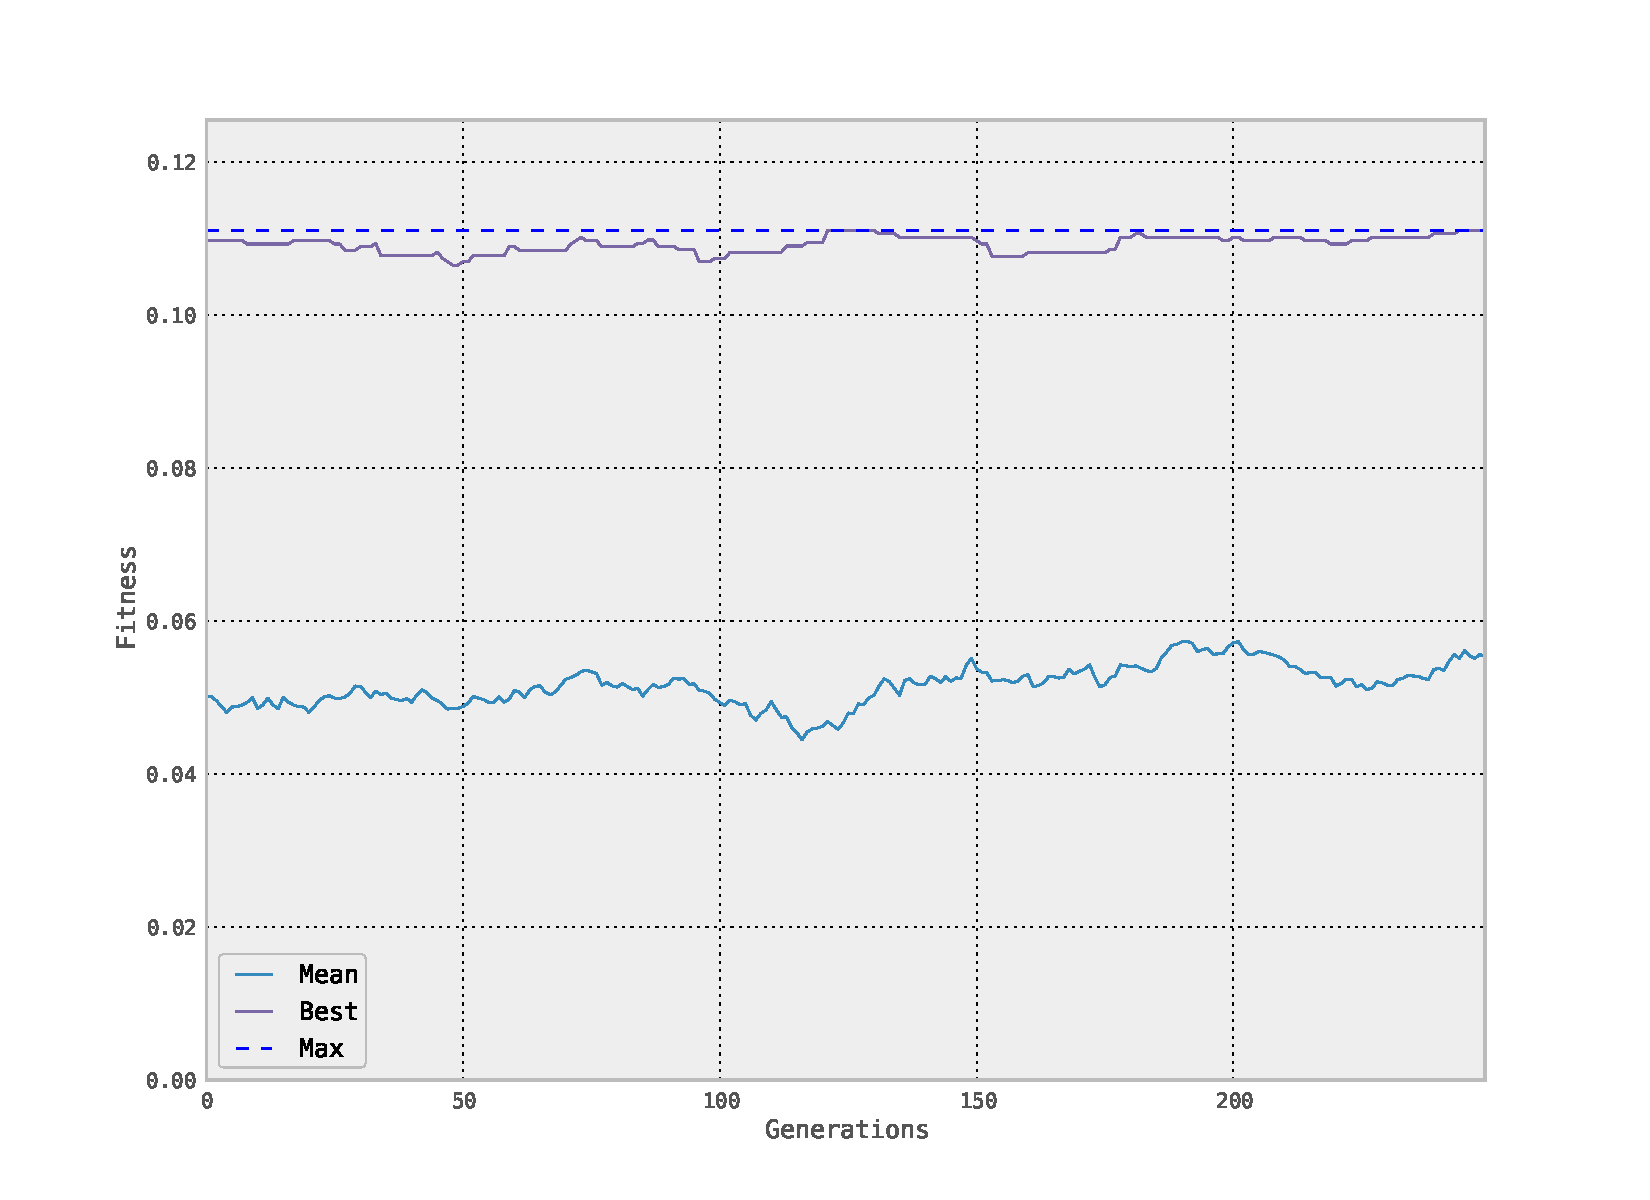
\includegraphics[scale =0.4] {images/section2/experimenta/fitness_15.pdf}
	\label{fig:subfig11}
}
\subfigure[Pheromones per edge]{
	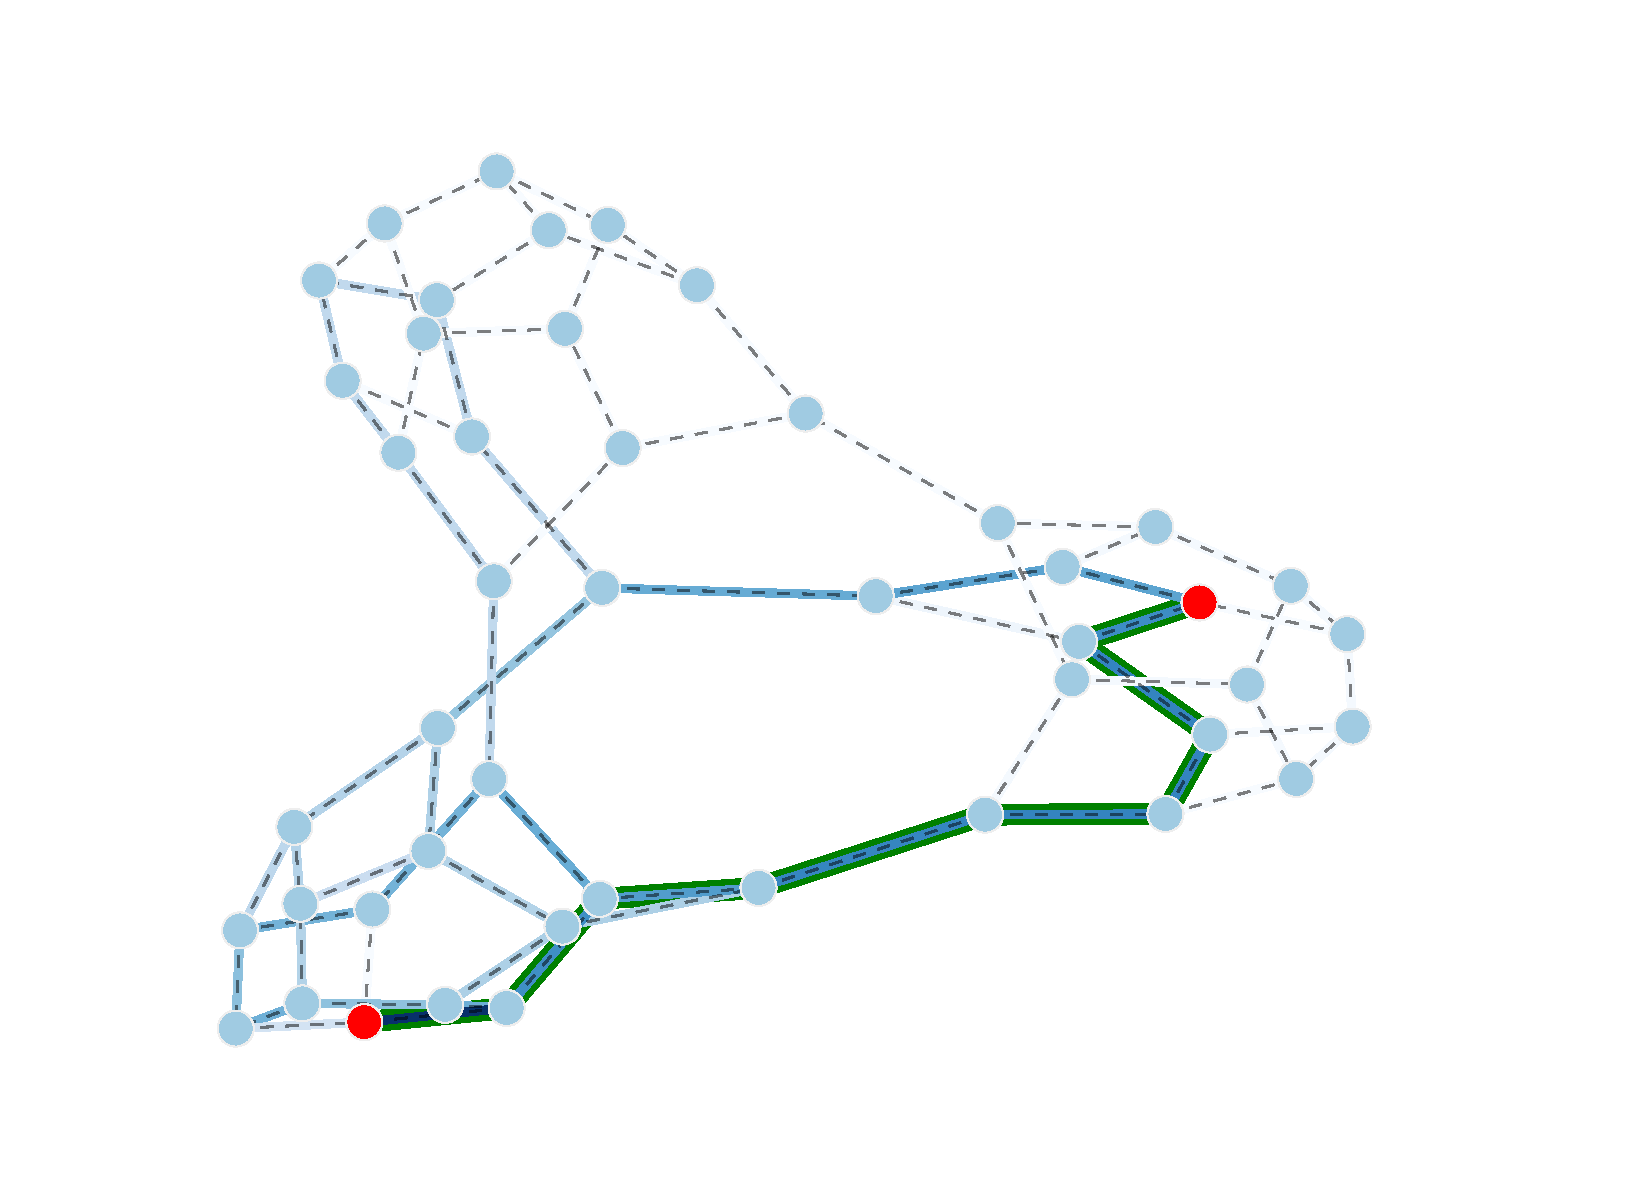
\includegraphics[scale =0.4] {images/section2/experimenta/pheromones_15_.pdf}
	\label{fig:subfig12}
}
%\caption[Optional caption for list of figures]{Caption of subfigures \subref{fig:subfig1}, \subref{fig:subfig2}}
\label{fig:fig1}
\end{figure}

\newpage
\subsubsection{Ant-like I, $k=50$}

\begin{figure}[ht]
\centering
\subfigure[Fitness evolution]{
	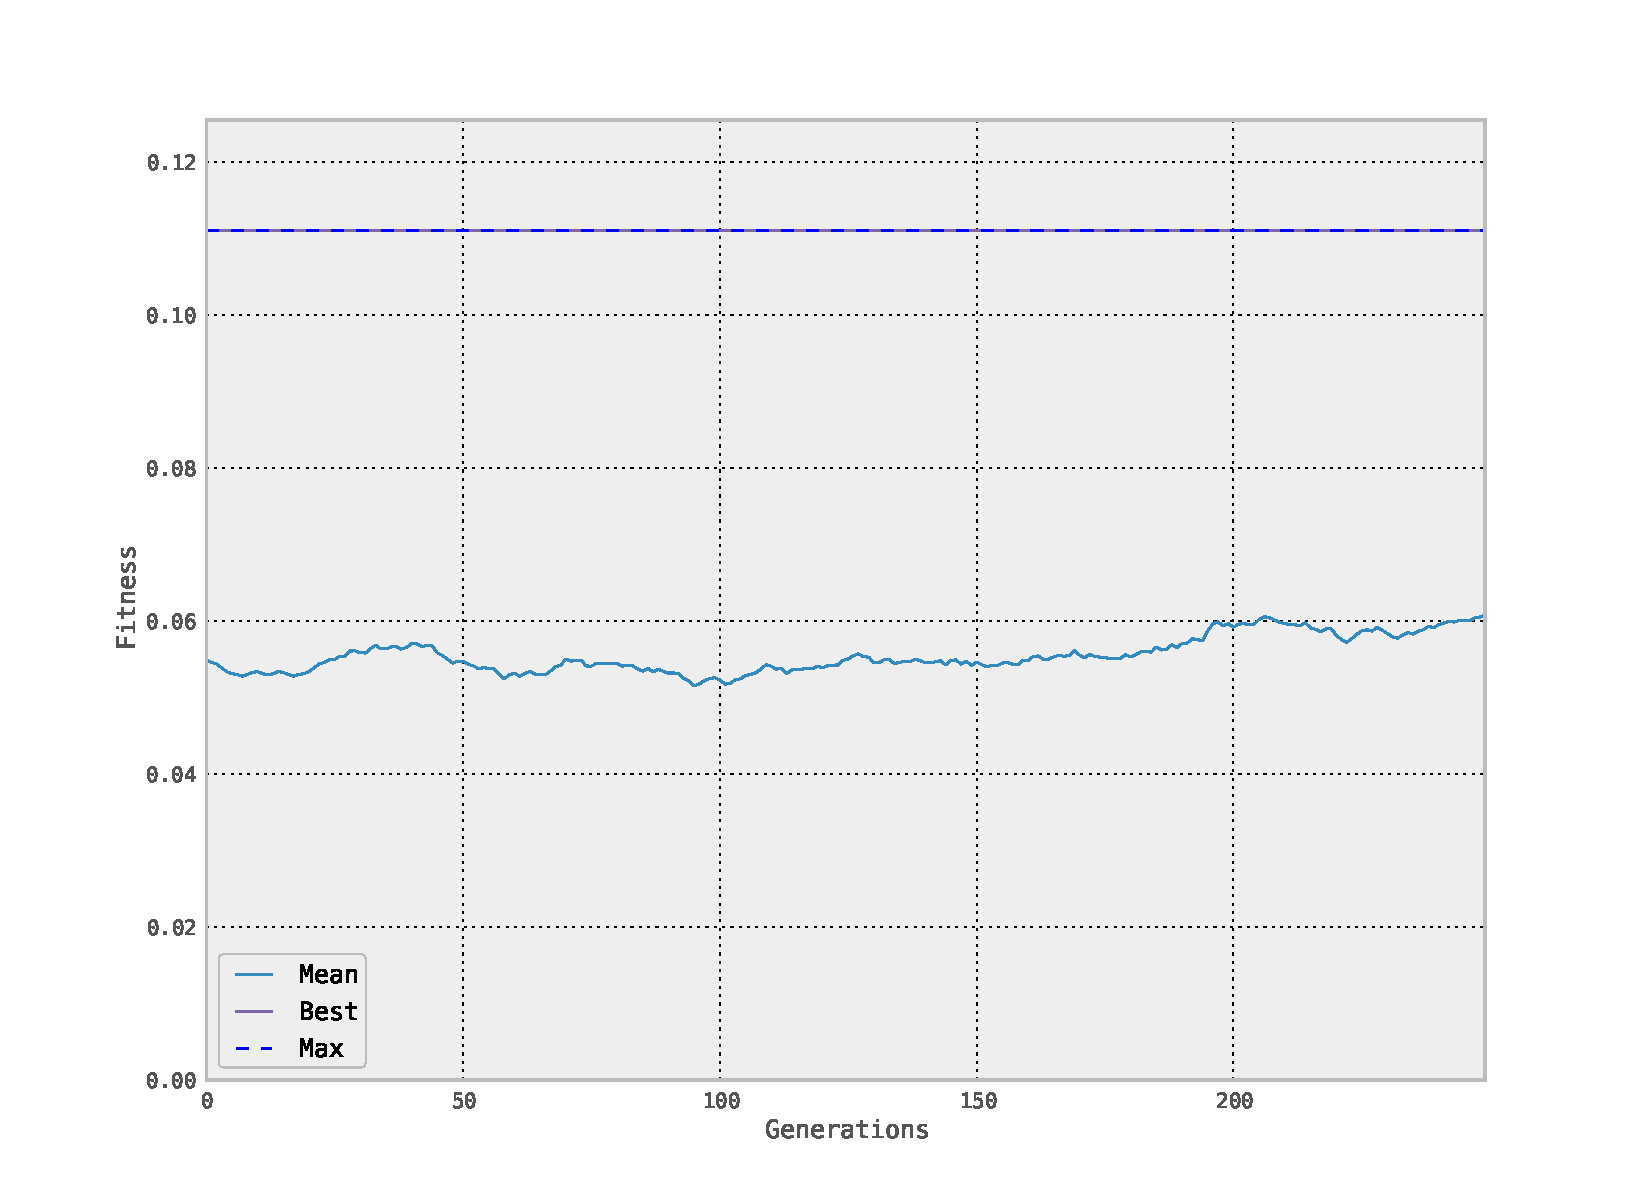
\includegraphics[scale =0.4] {images/section2/experimenta/fitness_50.pdf}
	\label{fig:subfig11}
}
\subfigure[Pheromones per edge]{
	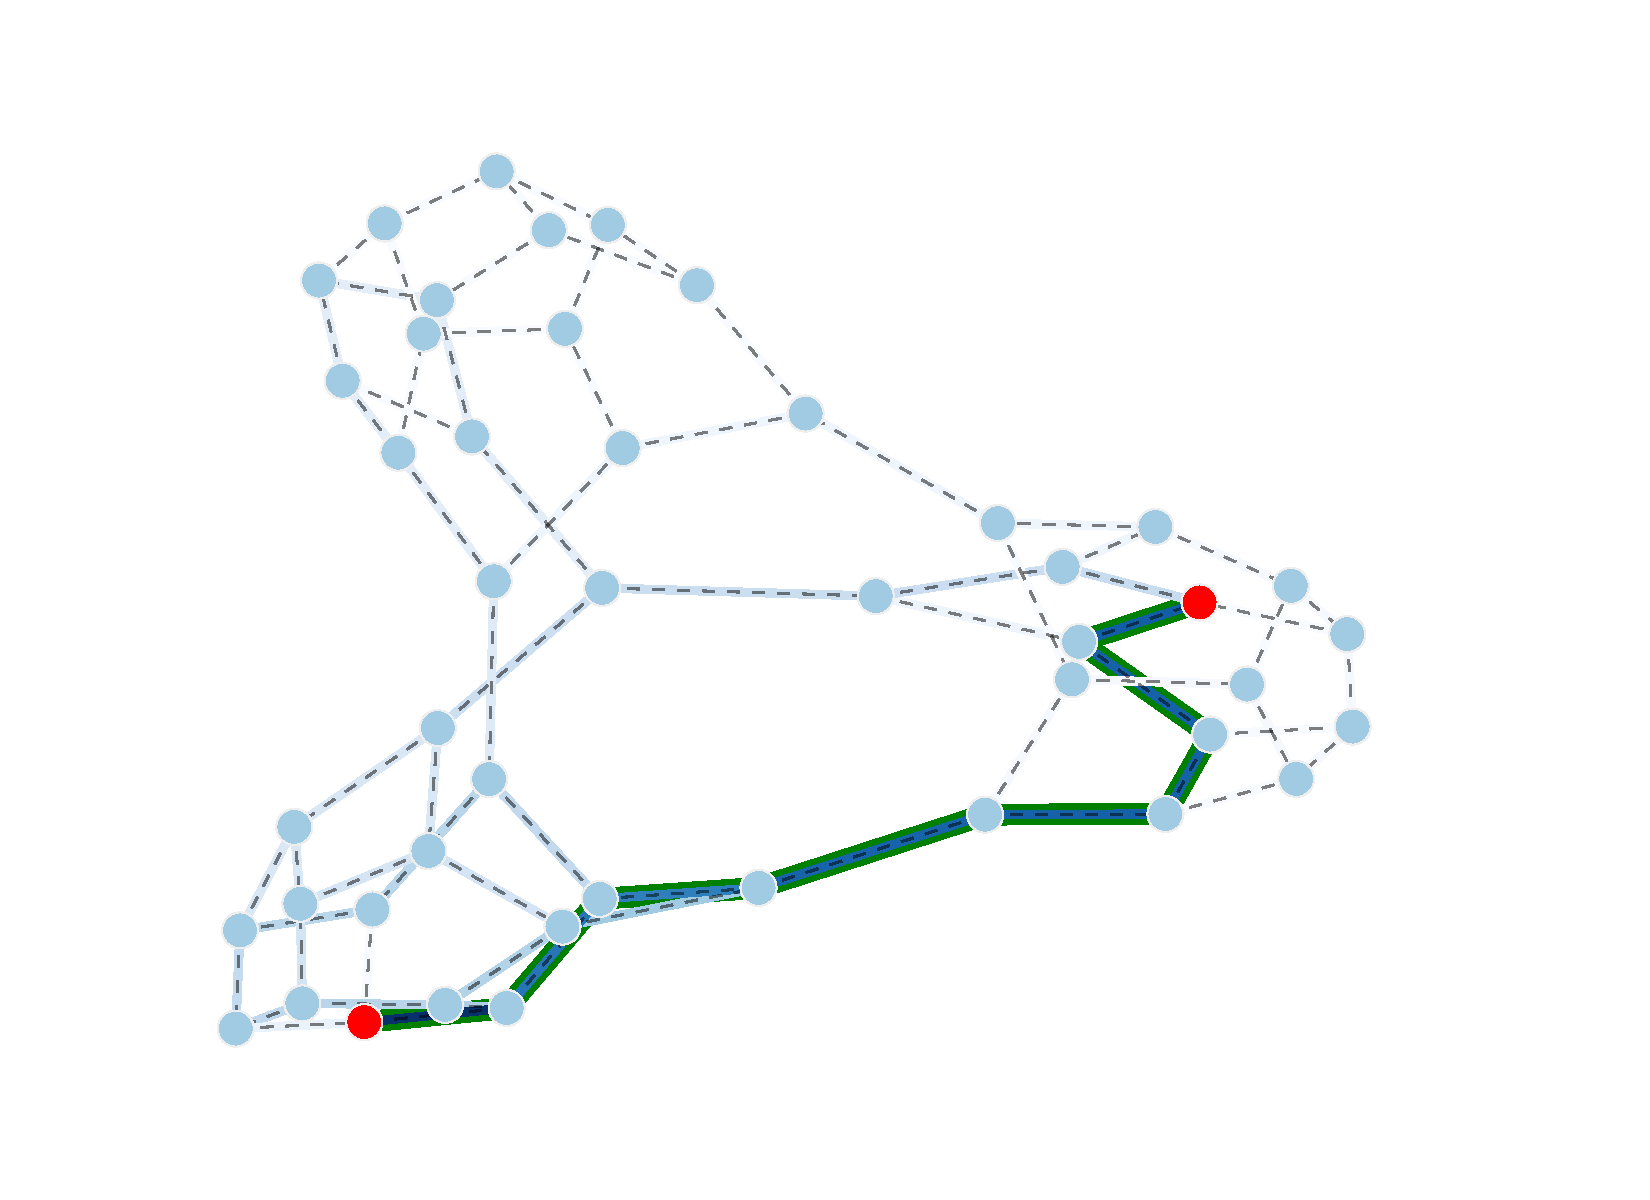
\includegraphics[scale =0.4] {images/section2/experimenta/pheromones_50_.pdf}
	\label{fig:subfig12}
}
%\caption[Optional caption for list of figures]{Caption of subfigures \subref{fig:subfig1}, \subref{fig:subfig2}}
\label{fig:fig1}
\end{figure}


\newpage
\subsubsection{Ant-like I, $k=100$}

\begin{figure}[ht]
\centering
\subfigure[Fitness evolution]{
	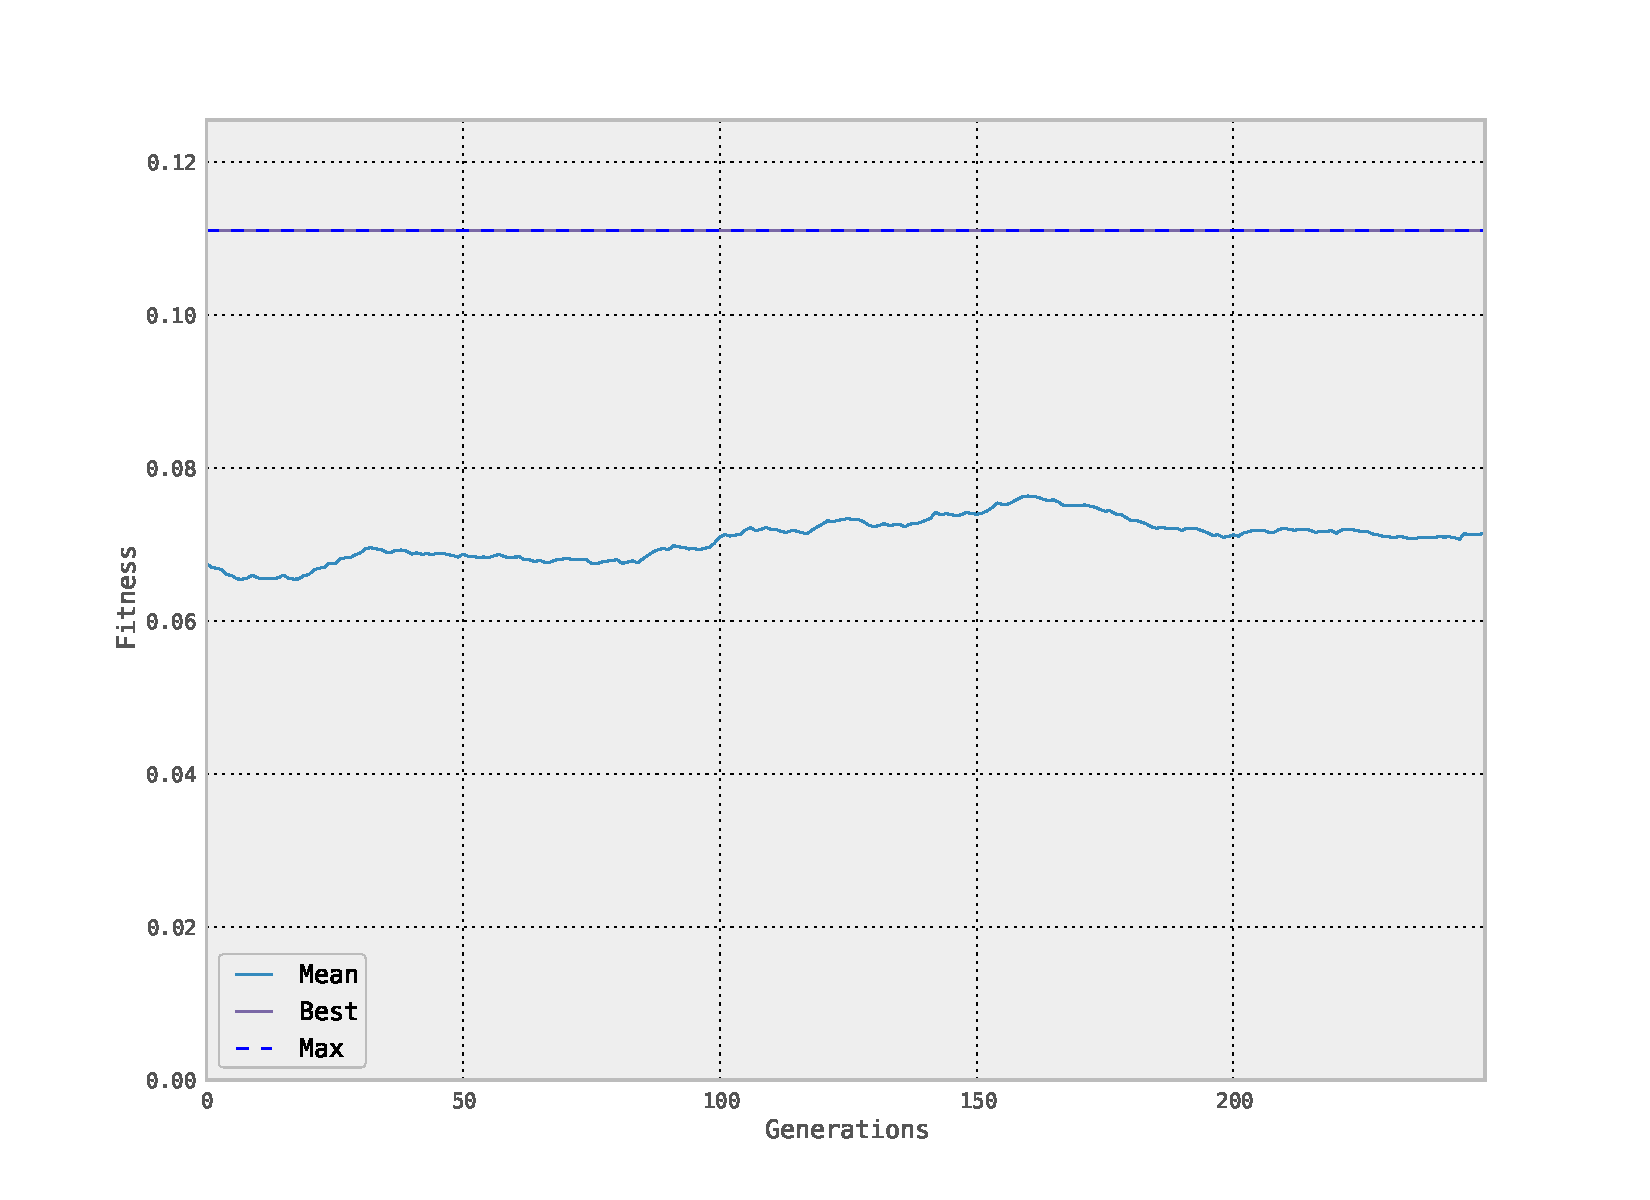
\includegraphics[scale =0.4] {images/section2/experimenta/fitness_100.pdf}
	\label{fig:subfig11}
}
\subfigure[Pheromones per edge]{
	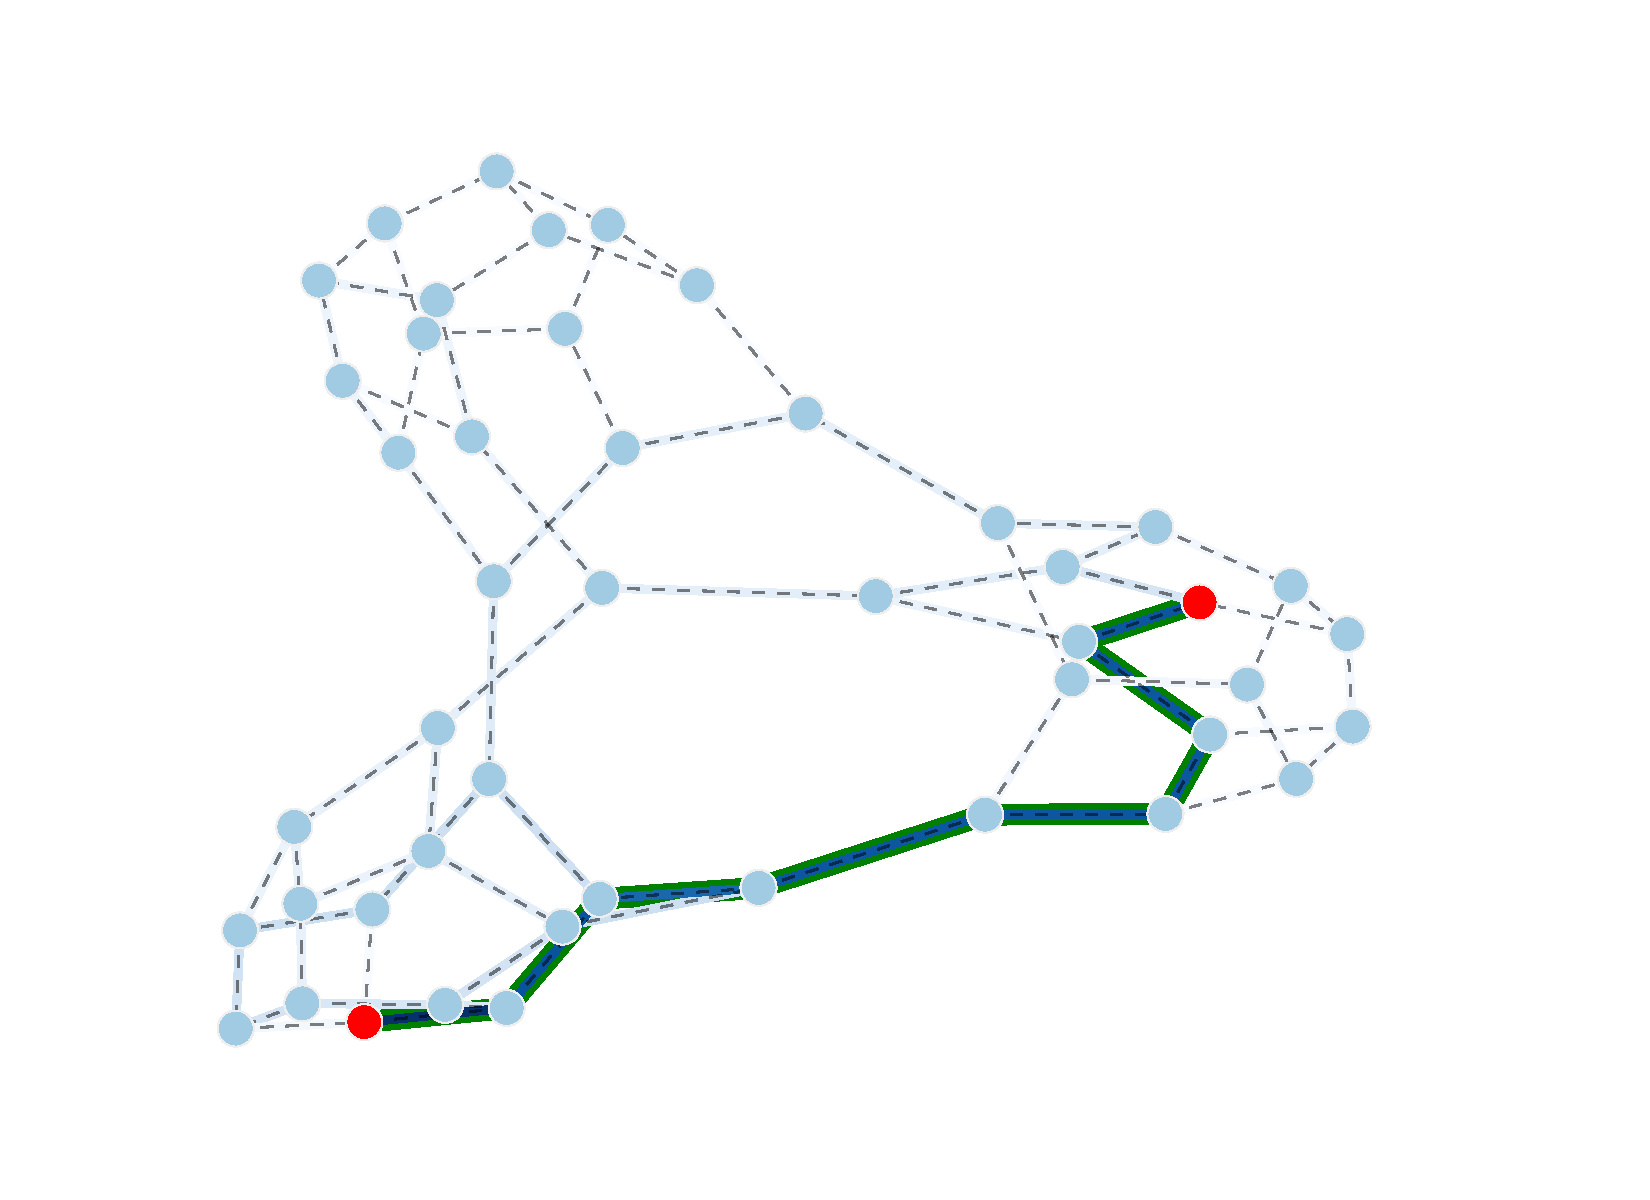
\includegraphics[scale =0.4] {images/section2/experimenta/pheromones_100_.pdf}
	\label{fig:subfig12}
}
%\caption[Optional caption for list of figures]{Caption of subfigures \subref{fig:subfig1}, \subref{fig:subfig2}}
\label{fig:fig1}
\end{figure}










\newpage
\subsubsection{Ant-like II, $k=5$}

\begin{figure}[ht]
\centering
\subfigure[Fitness evolution]{
	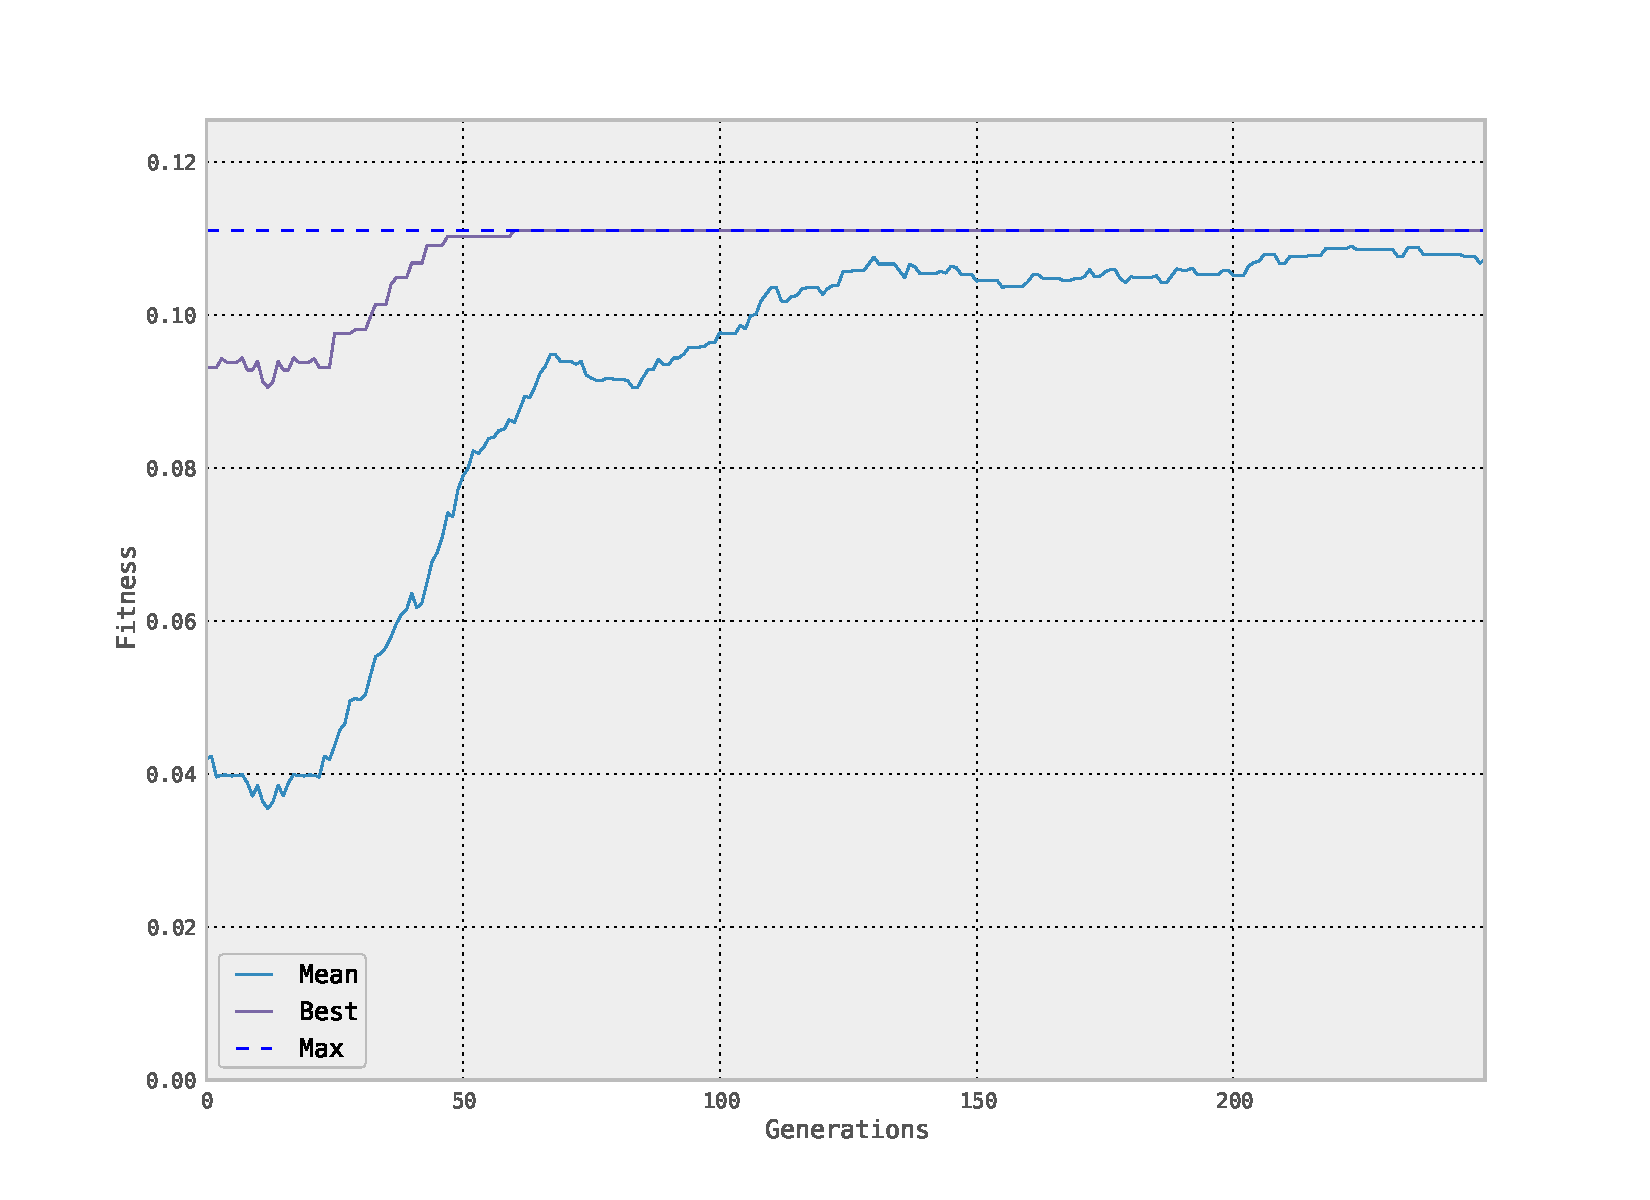
\includegraphics[scale =0.4] {images/section2/experimentb/fitness_5.pdf}
	\label{fig:subfig11}
}
\subfigure[Pheromones per edge]{
	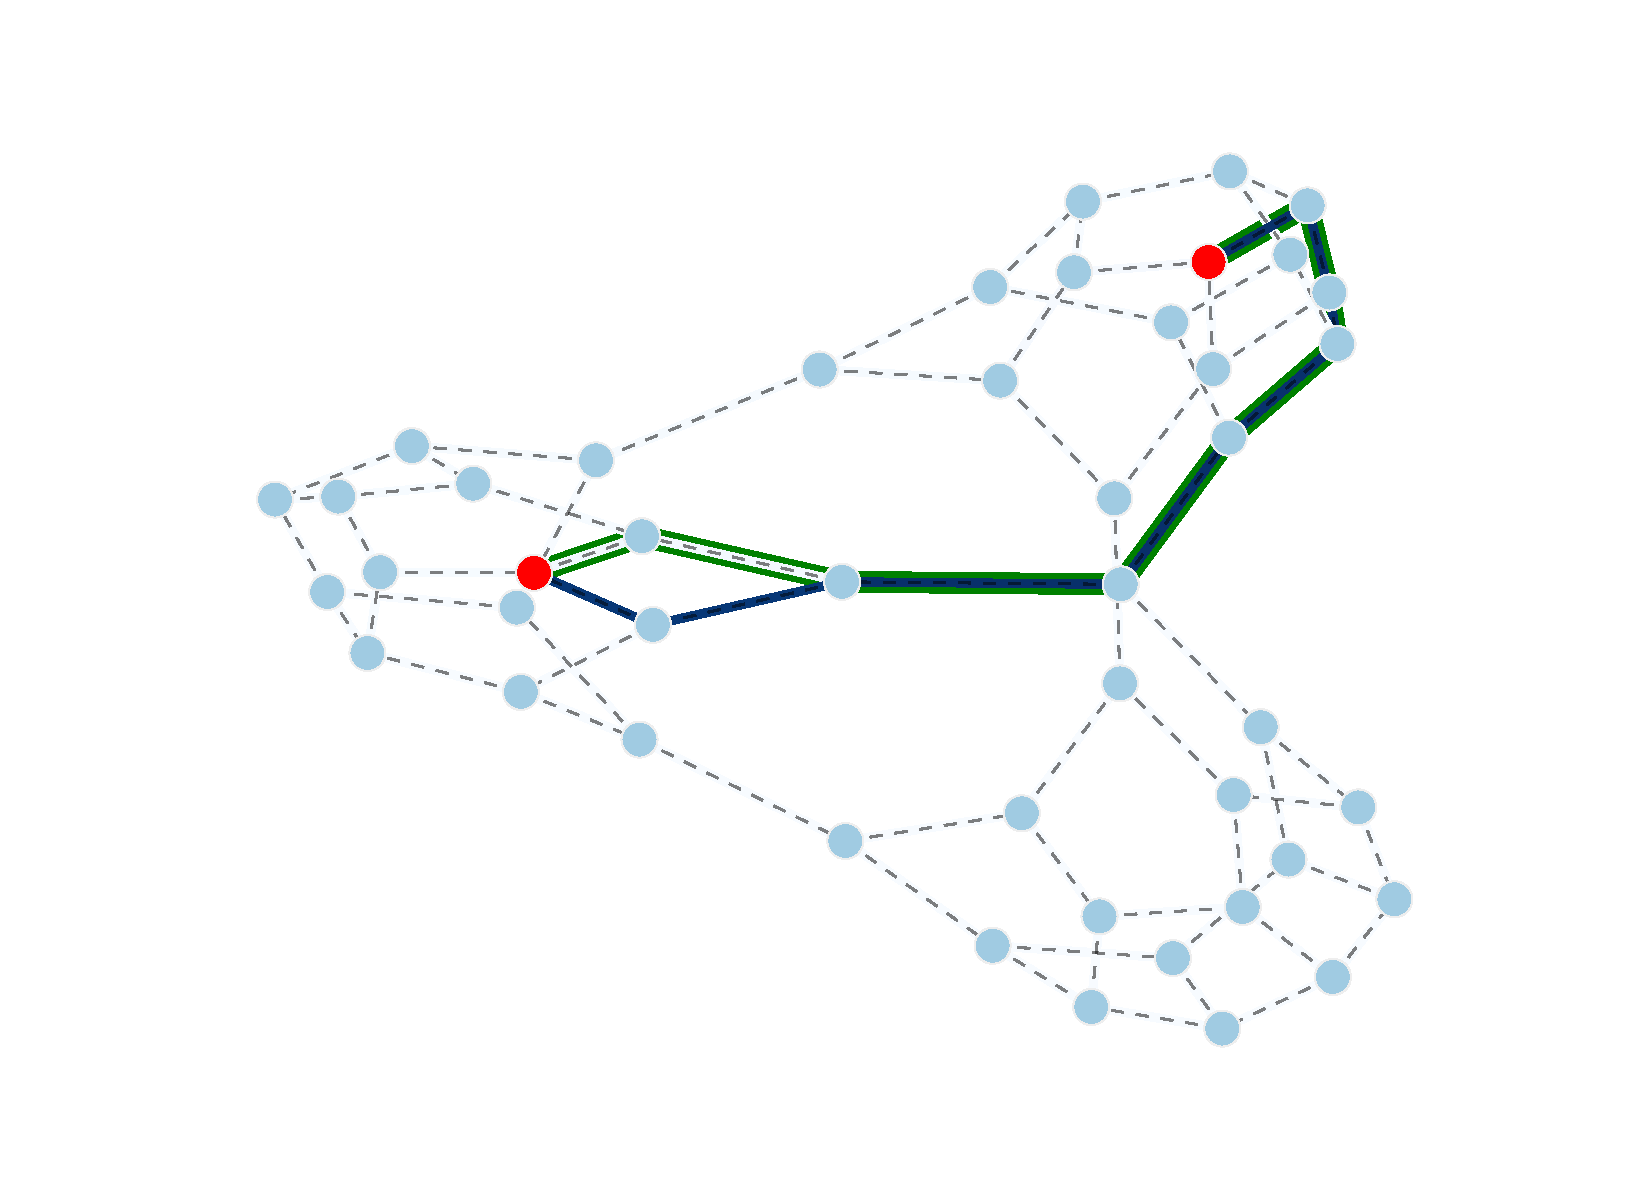
\includegraphics[scale =0.4] {images/section2/experimentb/pheromones_5_.pdf}
	\label{fig:subfig12}
}
%\caption[Optional caption for list of figures]{Caption of subfigures \subref{fig:subfig1}, \subref{fig:subfig2}}
\label{fig:fig1}
\end{figure}


\newpage
\subsubsection{Ant-like II, $k=10$}

\begin{figure}[ht]
\centering
\subfigure[Fitness evolution]{
	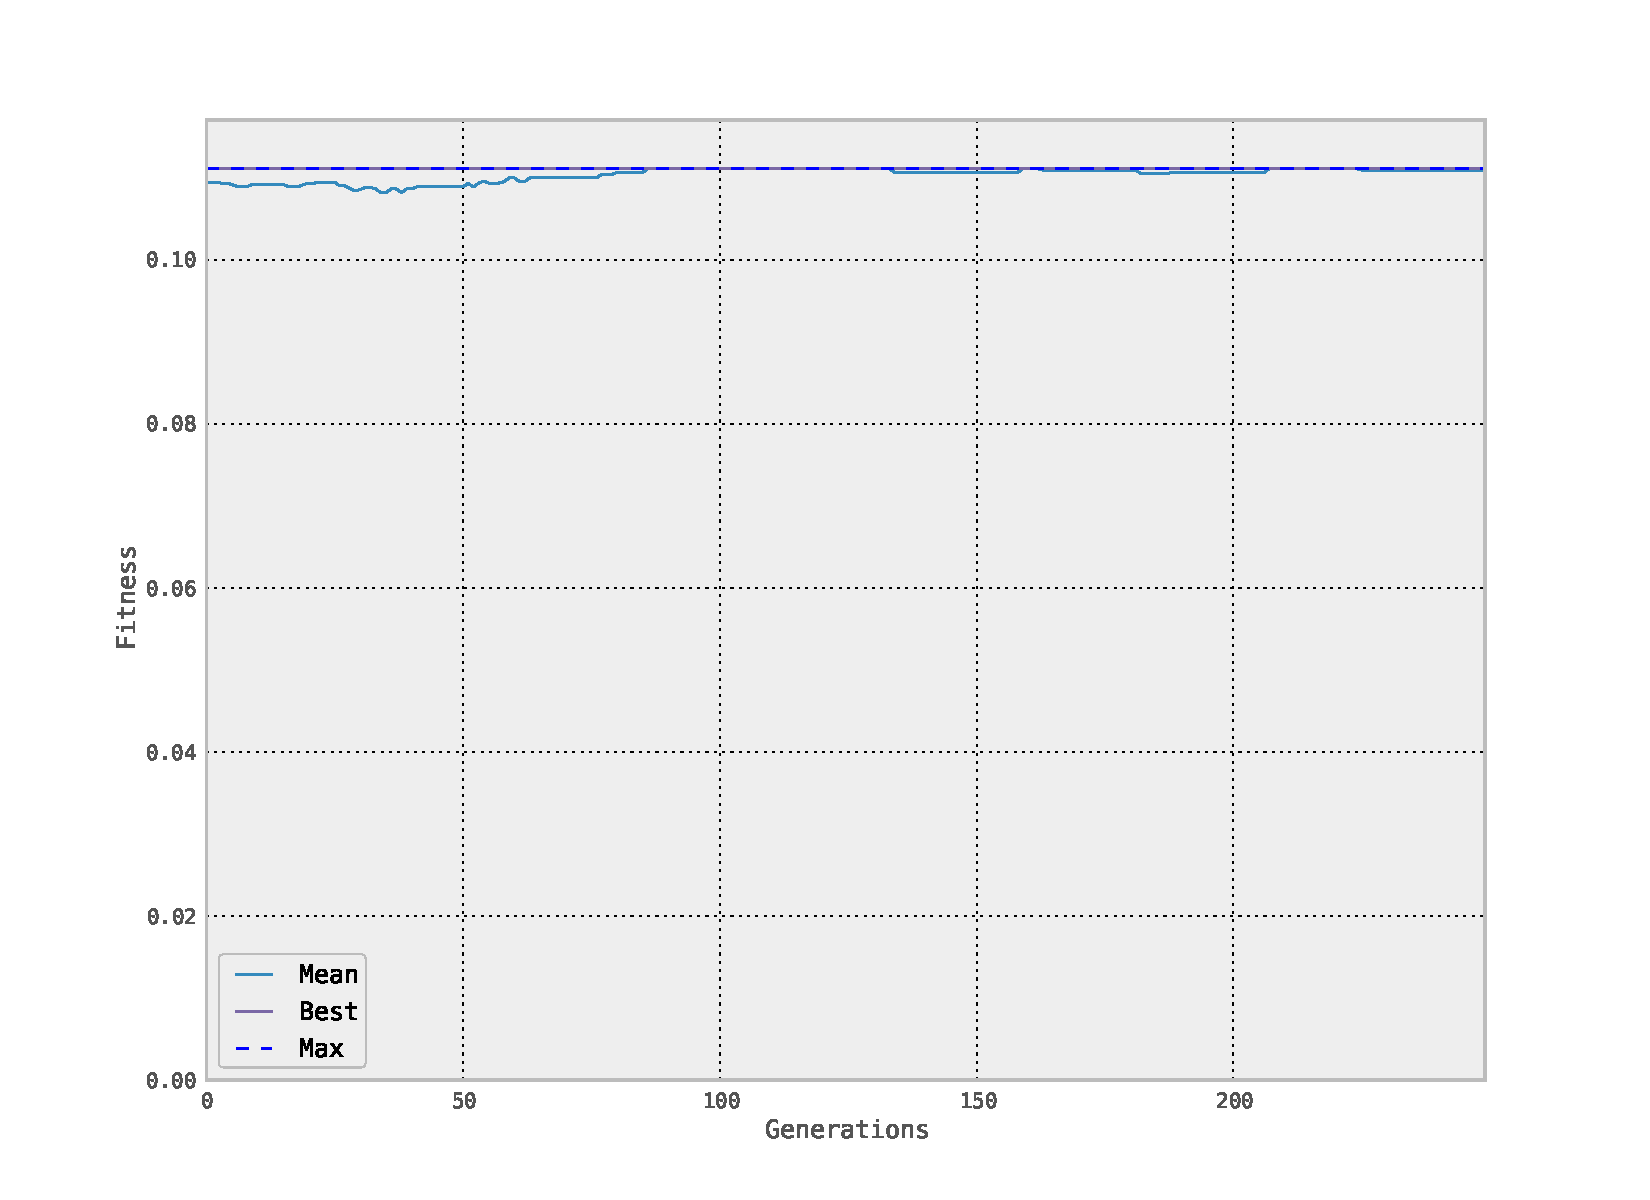
\includegraphics[scale =0.4] {images/section2/experimentb/fitness_10.pdf}
	\label{fig:subfig11}
}
\subfigure[Pheromones per edge]{
	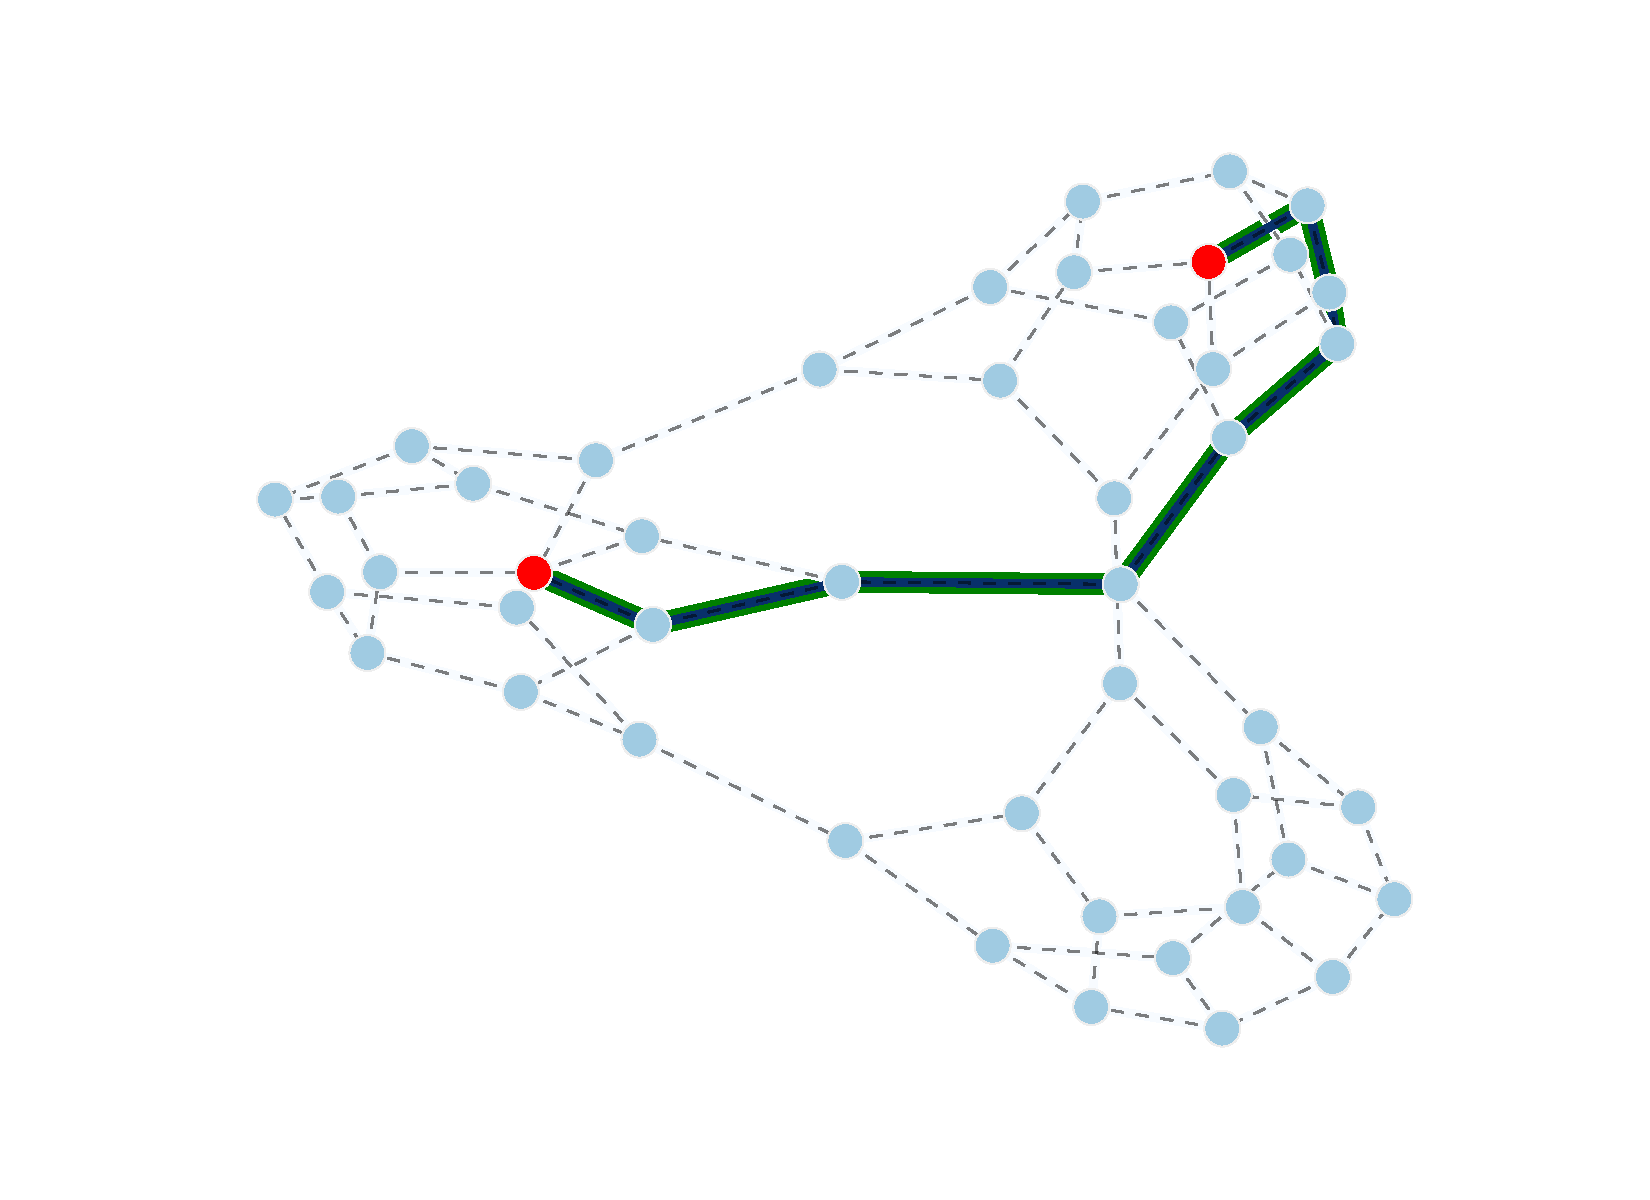
\includegraphics[scale =0.4] {images/section2/experimentb/pheromones_10_.pdf}
	\label{fig:subfig12}
}
%\caption[Optional caption for list of figures]{Caption of subfigures \subref{fig:subfig1}, \subref{fig:subfig2}}
\label{fig:fig1}
\end{figure}


\newpage
\subsubsection{Ant-like II, $k=15$}

\begin{figure}[ht]
\centering
\subfigure[Fitness evolution]{
	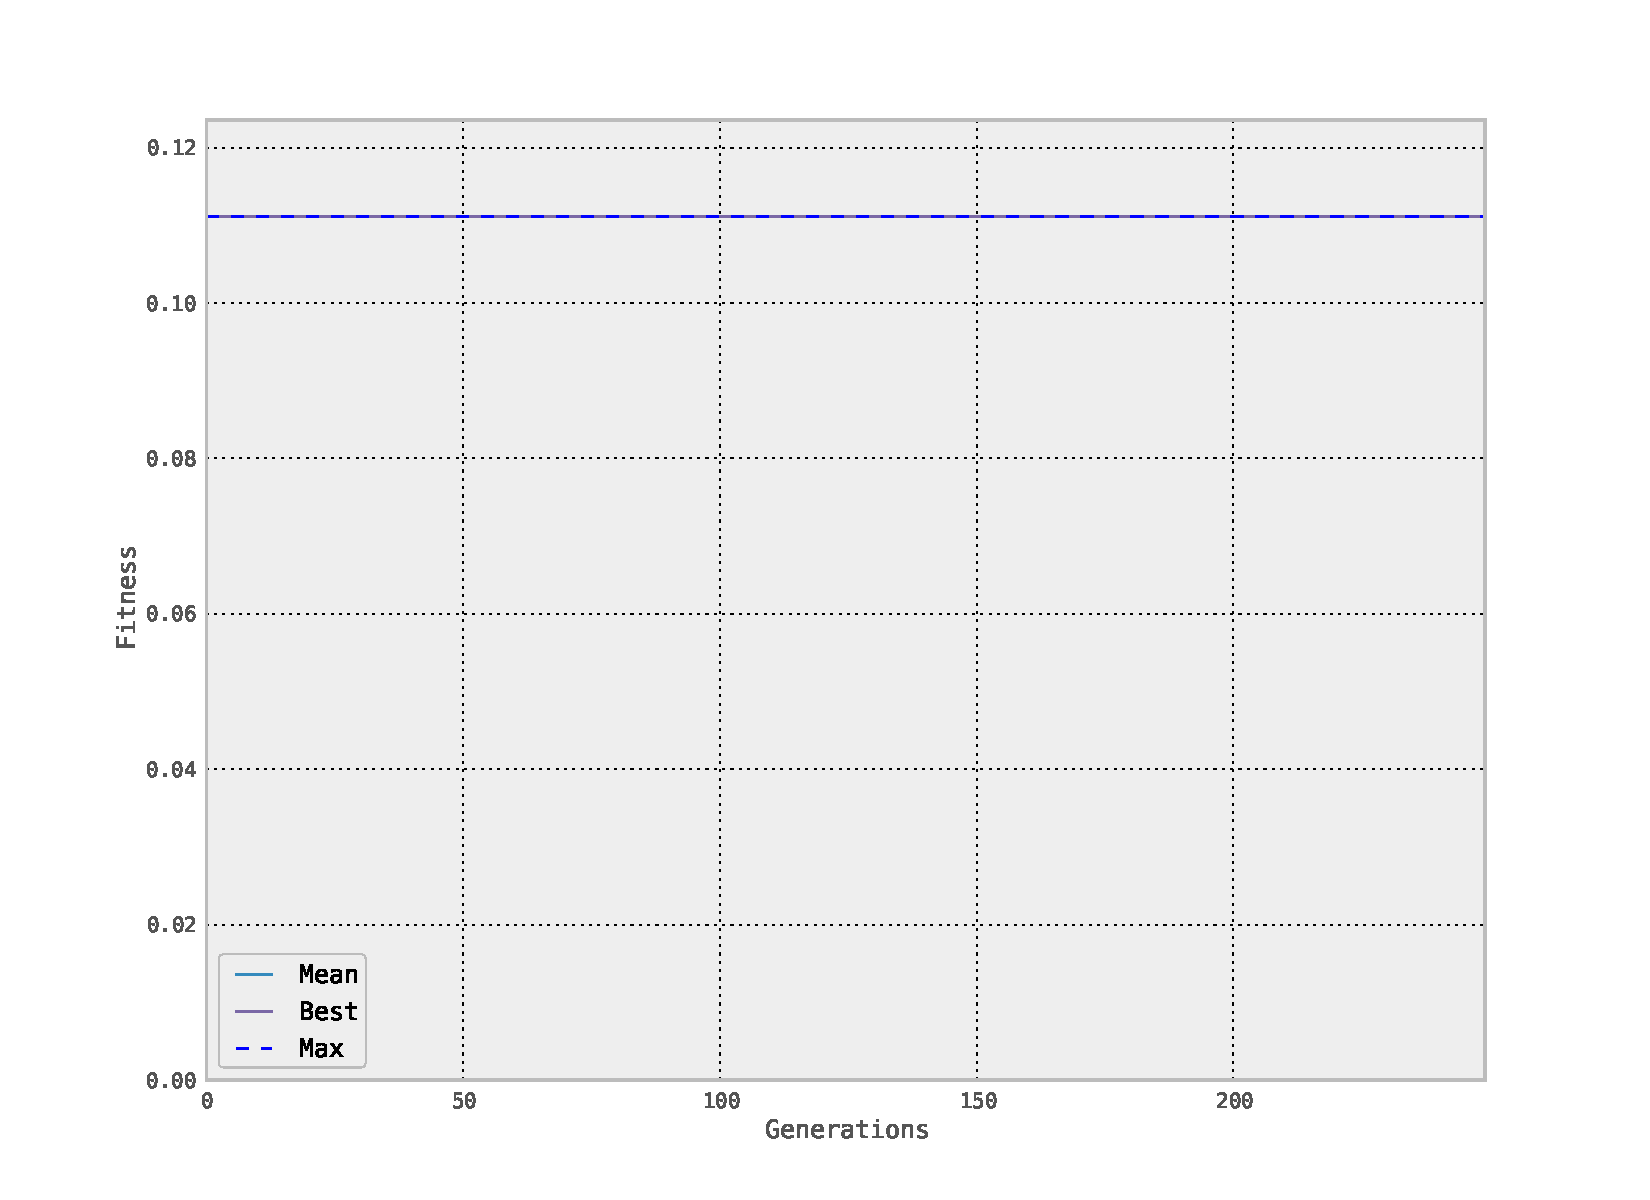
\includegraphics[scale =0.4] {images/section2/experimentb/fitness_15.pdf}
	\label{fig:subfig11}
}
\subfigure[Pheromones per edge]{
	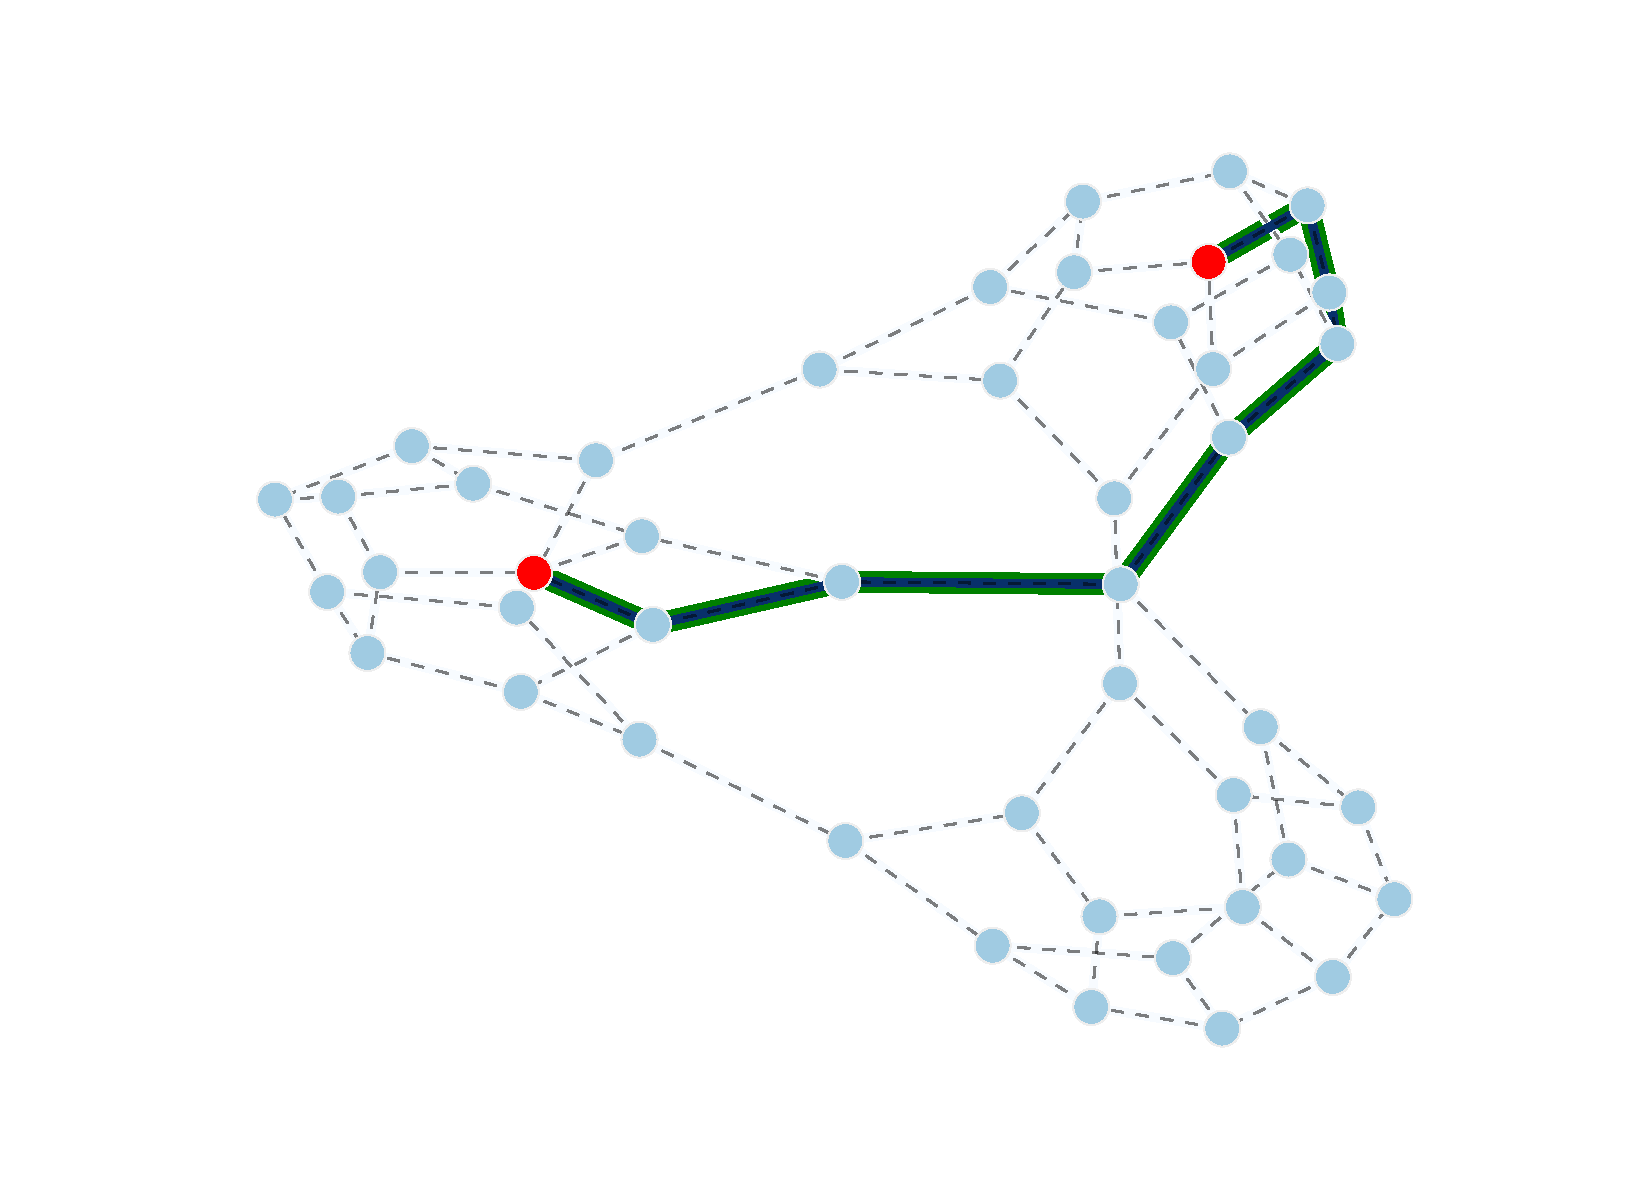
\includegraphics[scale =0.4] {images/section2/experimentb/pheromones_15_.pdf}
	\label{fig:subfig12}
}
%\caption[Optional caption for list of figures]{Caption of subfigures \subref{fig:subfig1}, \subref{fig:subfig2}}
\label{fig:fig1}
\end{figure}

\newpage
\subsubsection{Ant-like II, $k=50$}

\begin{figure}[ht]
\centering
\subfigure[Fitness evolution]{
	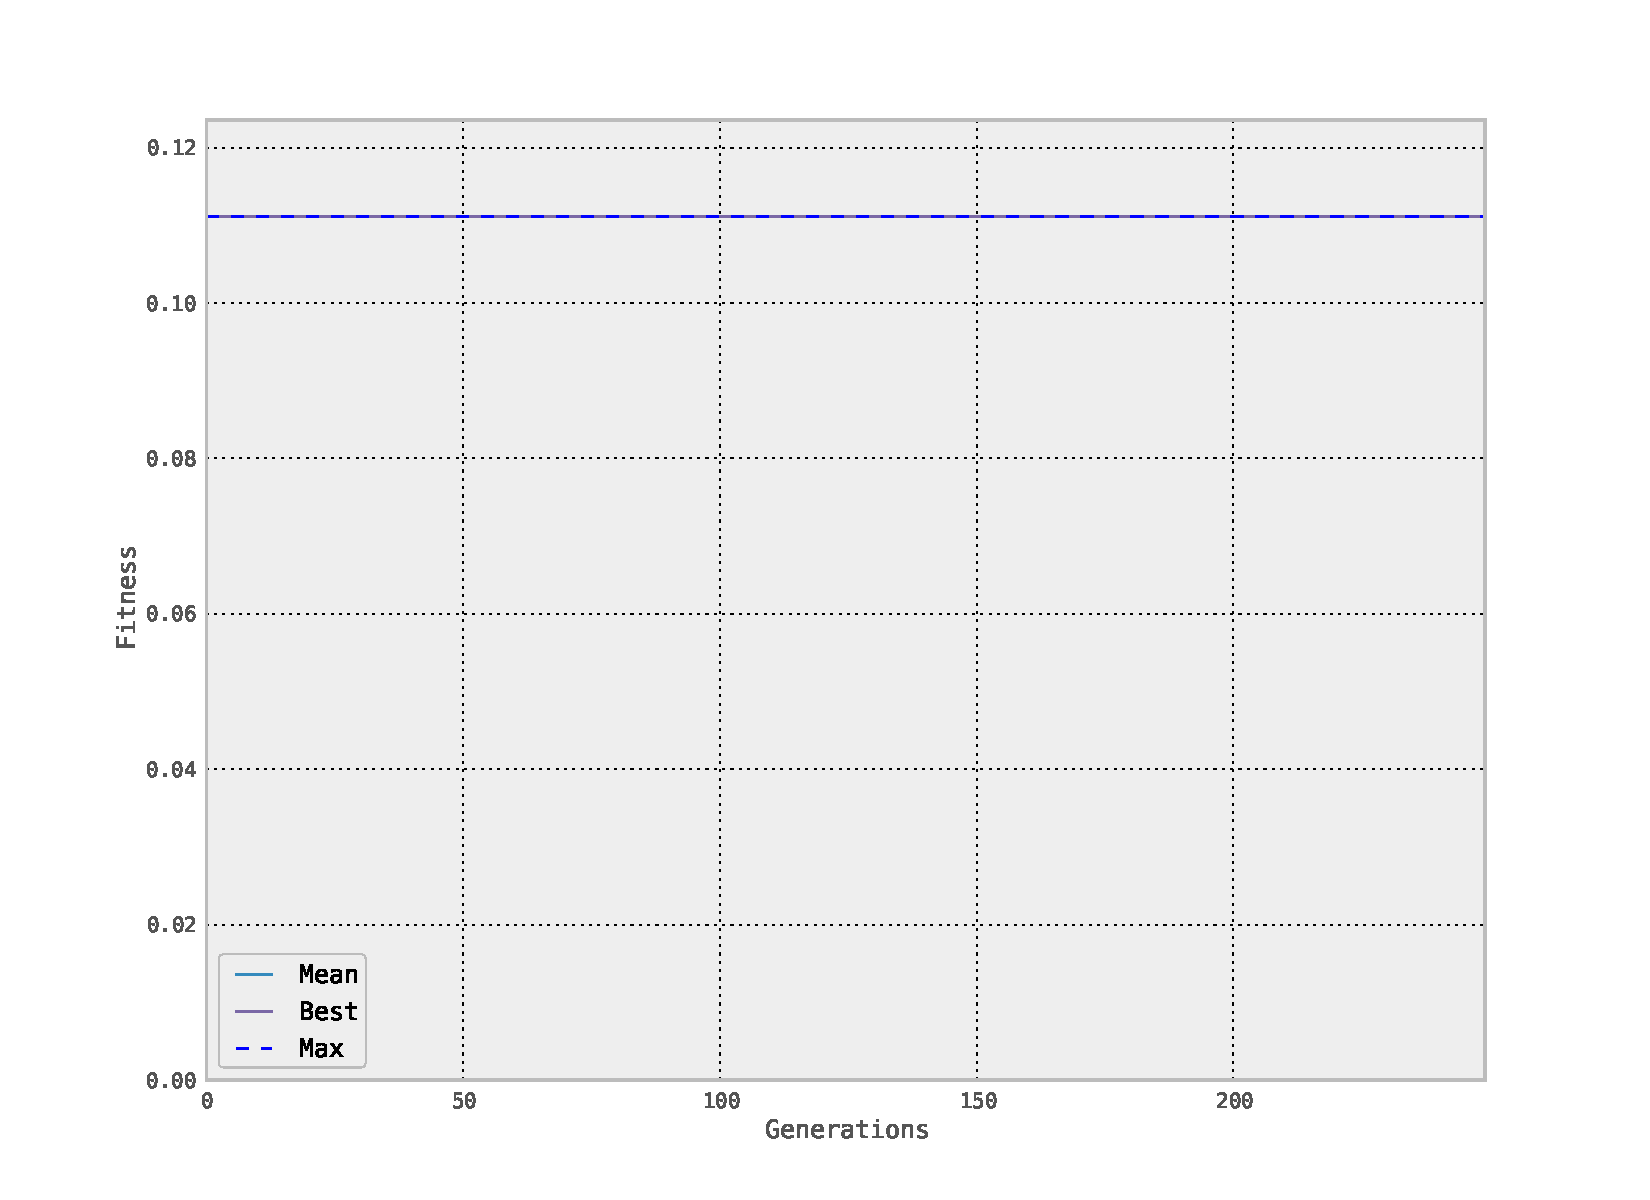
\includegraphics[scale =0.4] {images/section2/experimentb/fitness_50.pdf}
	\label{fig:subfig11}
}
\subfigure[Pheromones per edge]{
	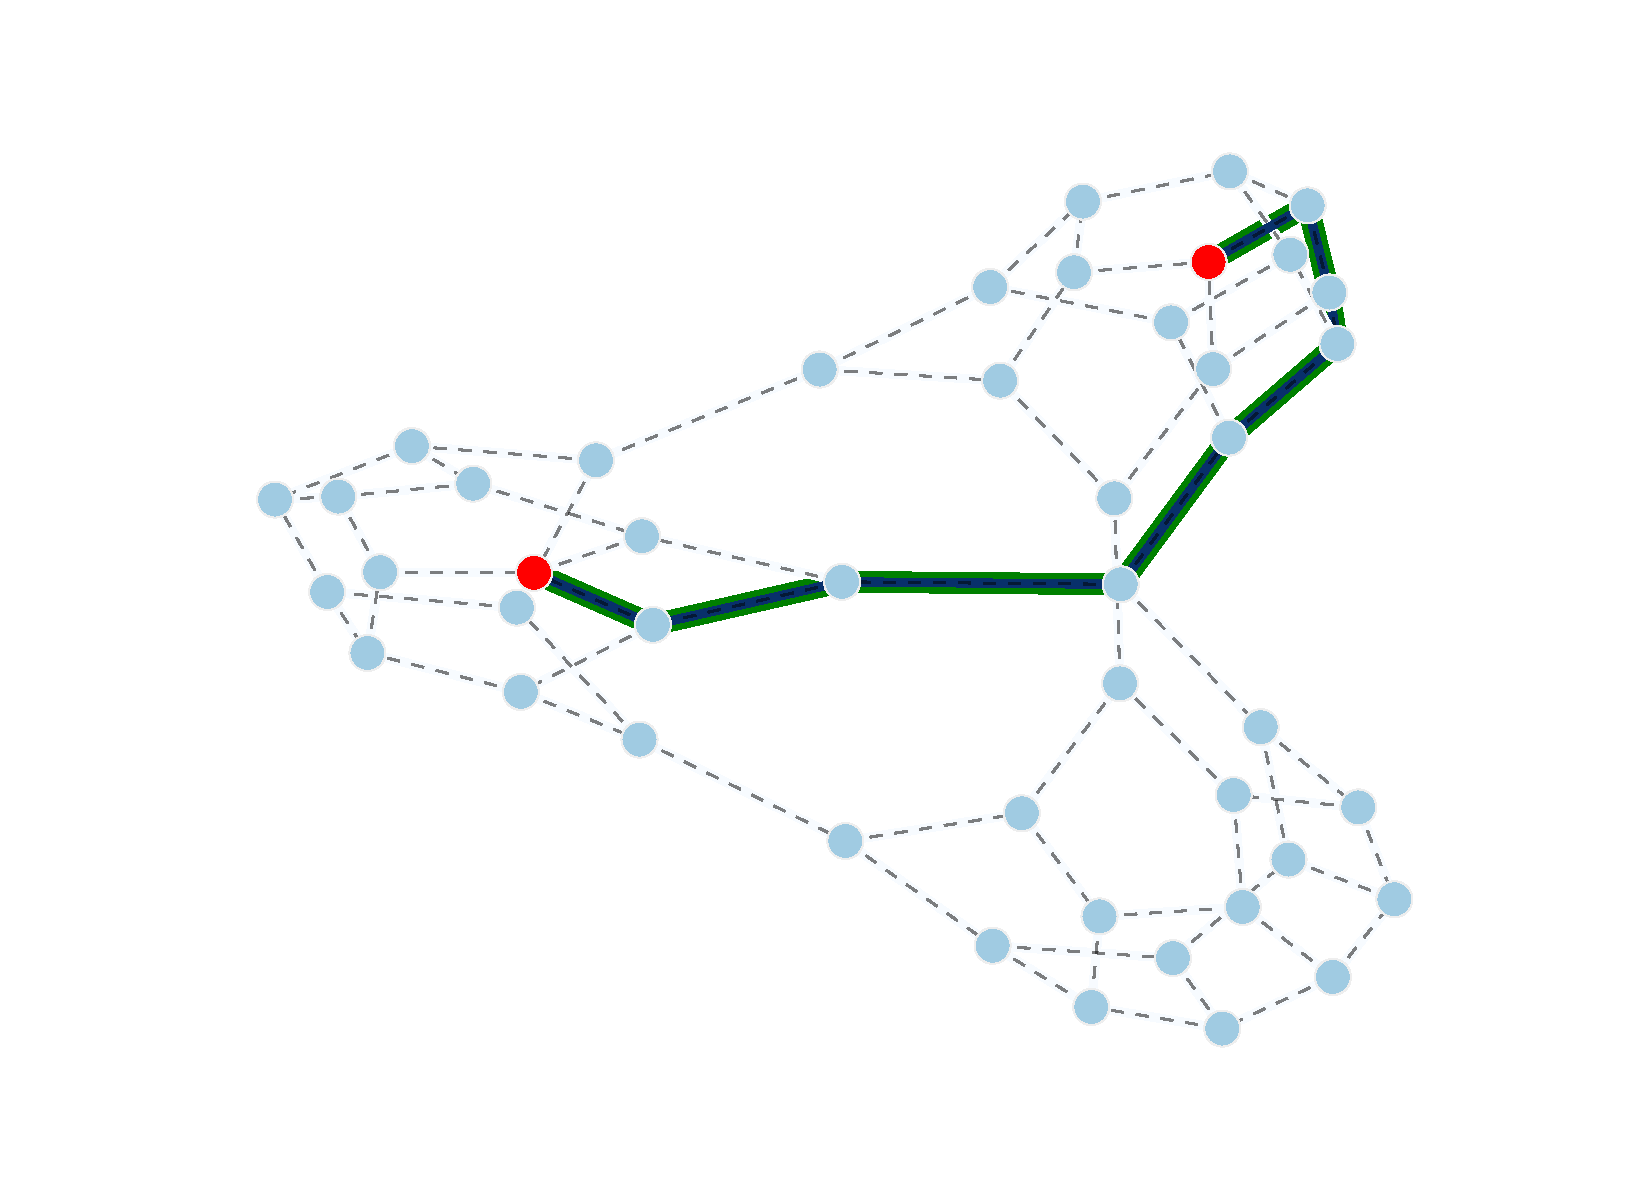
\includegraphics[scale =0.4] {images/section2/experimentb/pheromones_50_.pdf}
	\label{fig:subfig12}
}
%\caption[Optional caption for list of figures]{Caption of subfigures \subref{fig:subfig1}, \subref{fig:subfig2}}
\label{fig:fig1}
\end{figure}


\newpage
\subsubsection{Ant-like II, $k=100$}

\begin{figure}[ht]
\centering
\subfigure[Fitness evolution]{
	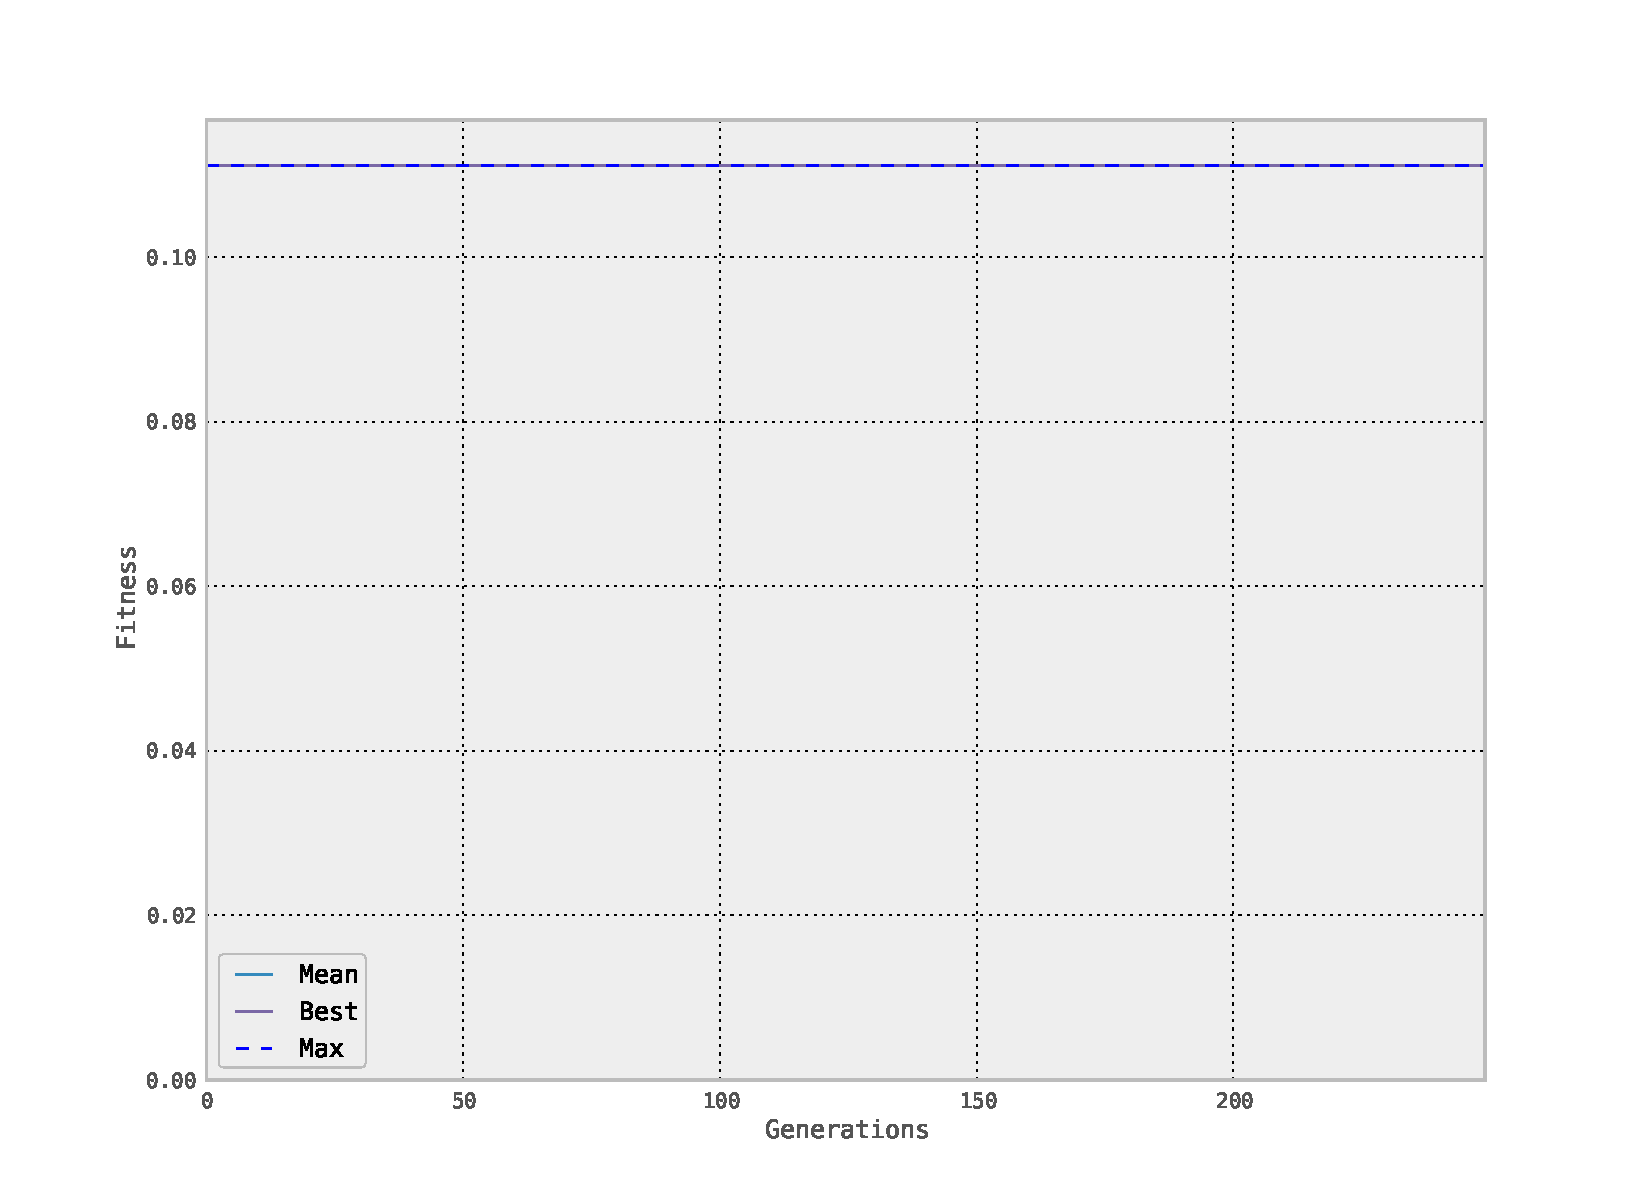
\includegraphics[scale =0.4] {images/section2/experimentb/fitness_100.pdf}
	\label{fig:subfig11}
}
\subfigure[Pheromones per edge]{
	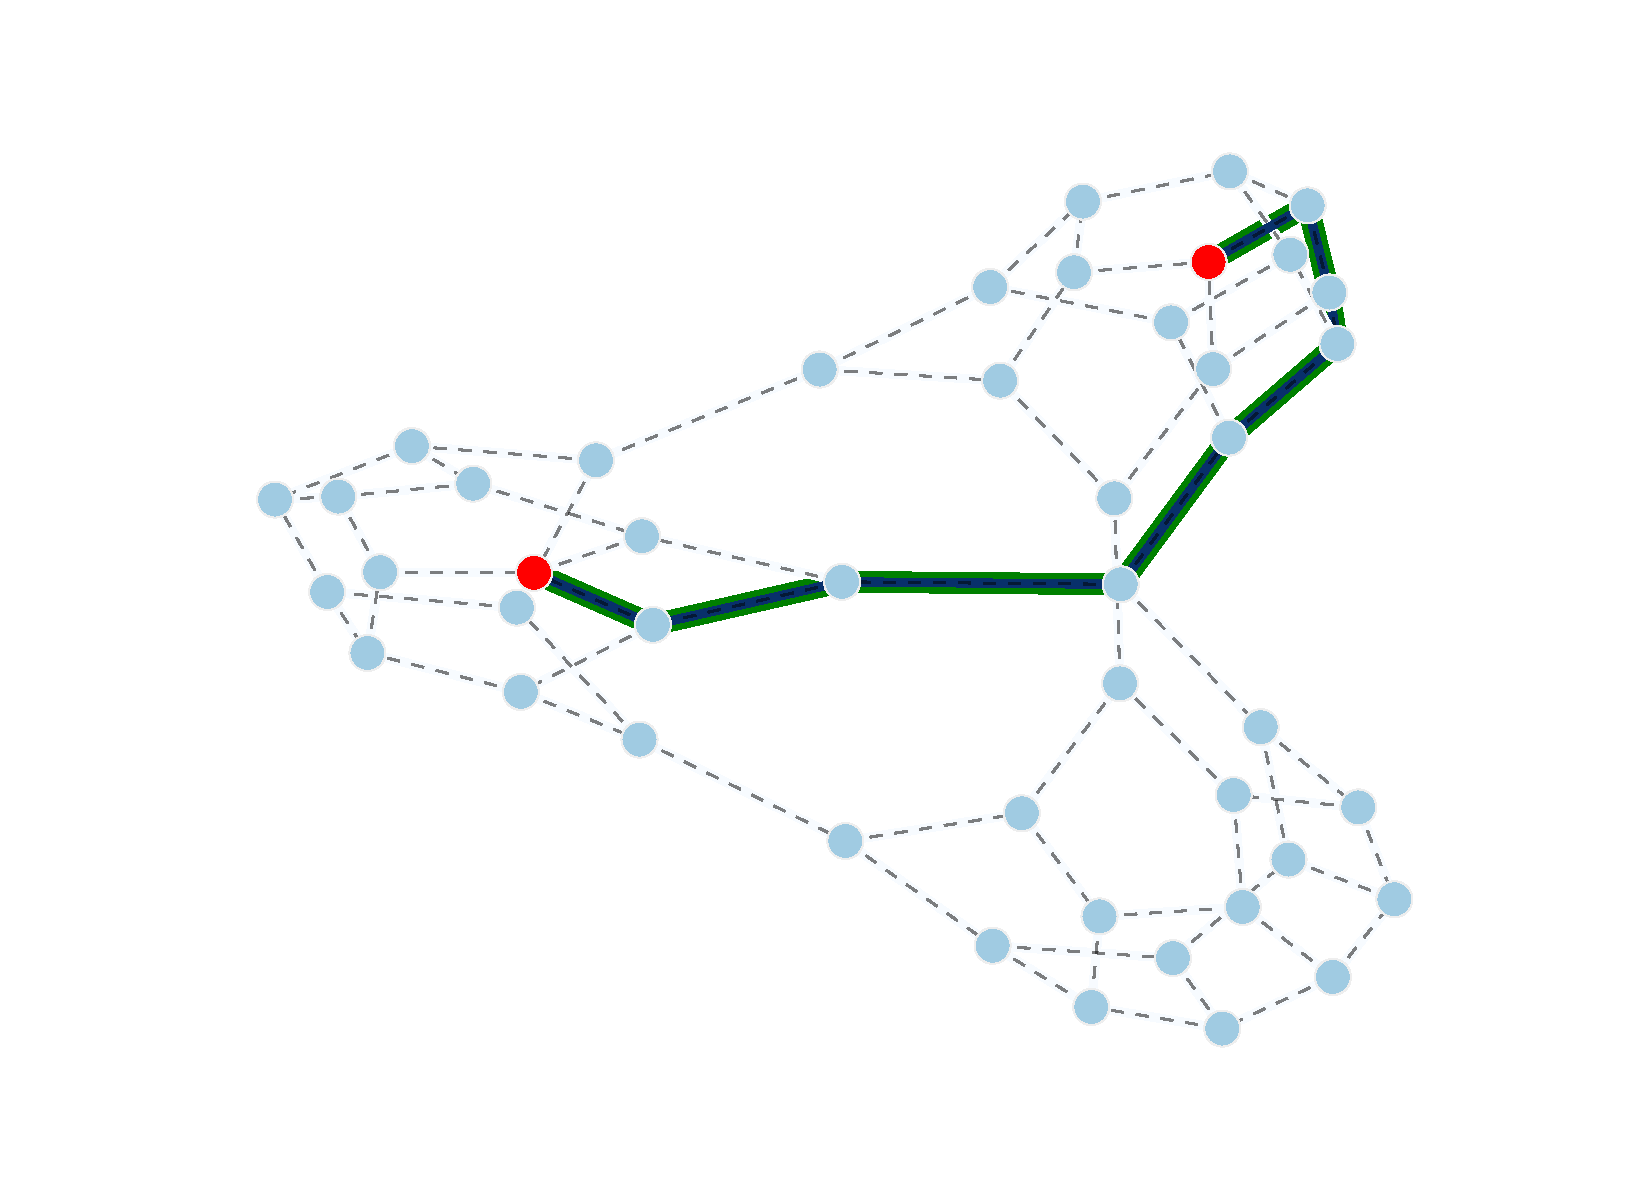
\includegraphics[scale =0.4] {images/section2/experimentb/pheromones_100_.pdf}
	\label{fig:subfig12}
}
%\caption[Optional caption for list of figures]{Caption of subfigures \subref{fig:subfig1}, \subref{fig:subfig2}}
\label{fig:fig1}
\end{figure}



\newpage
\subsection{Conclusions}
Ant-like I algorithm perform a better exploration, as we increase the variable $k$ from $5$ to $100$ the exploration decreases. Ant-like Ii algorithm always reach the best path, with $k=5$ we can get a suboptimal path near the optimal one, however, from $k=10$ to $k=100$ the best path is always reached.
\newpage
\section{Colective exploration algorithms type I \& II analysis}

Several test have been done by means of $\rho$ and $k$ combinations taken values in the next sets: $$\rho = \{0.01, 0.5\}, k = \{5, 10, 15, 50, 100\}$$

\subsection{Set $\rho = 0.1, k=5$}

\begin{figure}[ht]
\centering
\subfigure[Fitness evolution]{
	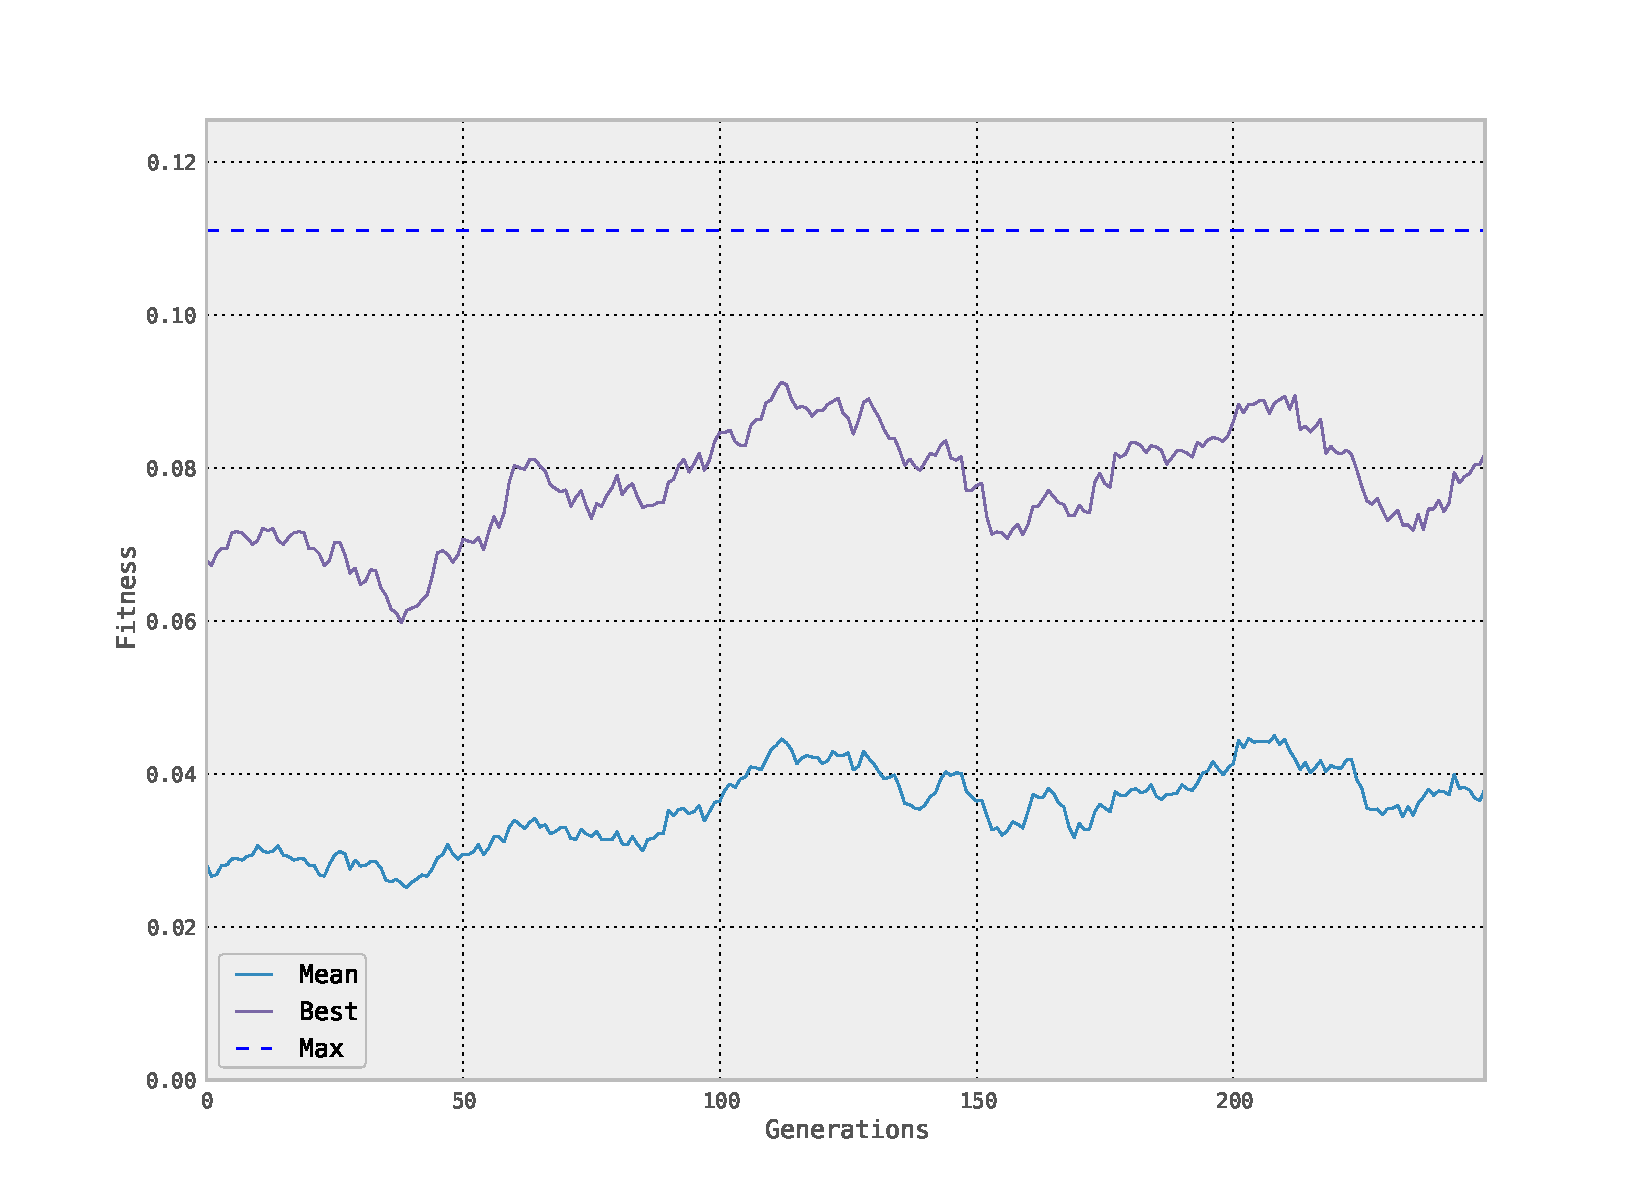
\includegraphics[scale =0.4] {images/section3/fitness_1_5_001.pdf}
	\label{fig:subfig11}
}
\subfigure[Pheromones per edge]{
	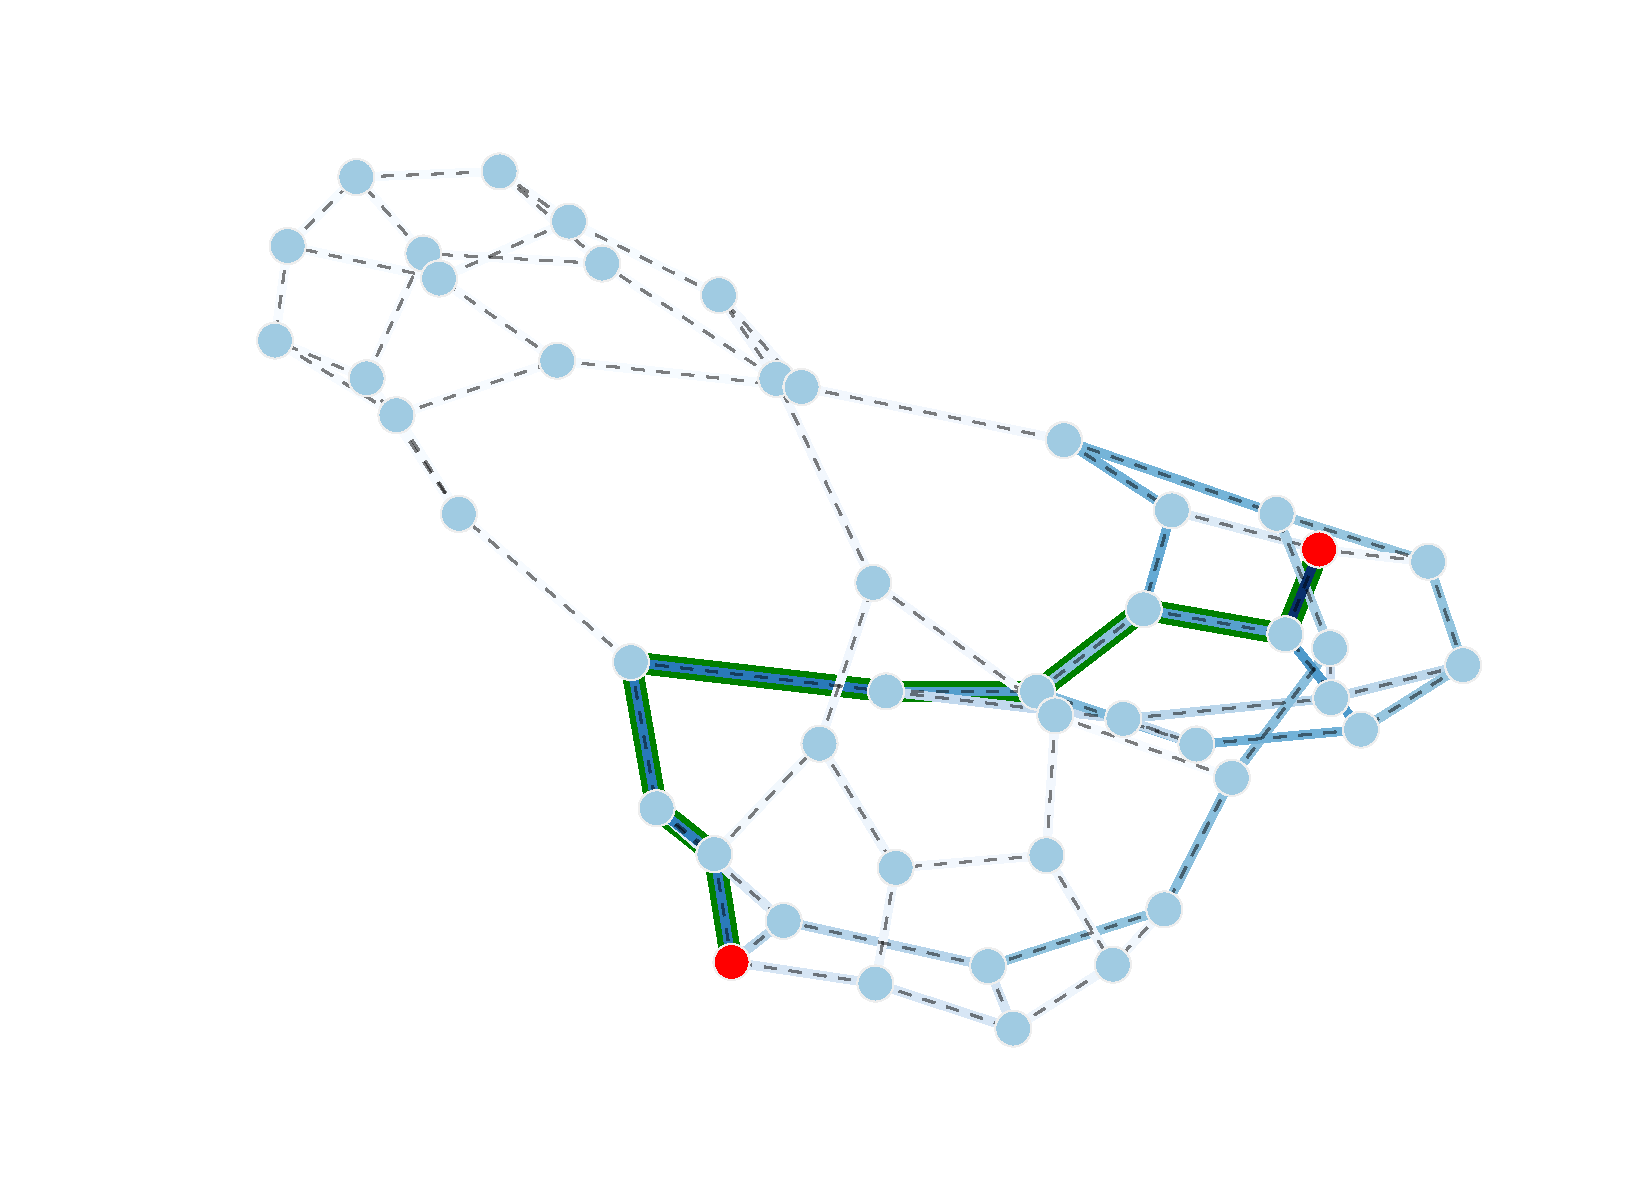
\includegraphics[scale =0.4] {images/section3/pheromones_5_001.pdf}
	\label{fig:subfig12}
}
%\caption[Optional caption for list of figures]{Caption of subfigures \subref{fig:subfig1}, \subref{fig:subfig2}}
\label{fig:fig1}
\end{figure}


\newpage
\subsection{Set $\rho = 0.1, k=10$}

\begin{figure}[ht]
\centering
\subfigure[Fitness evolution]{
	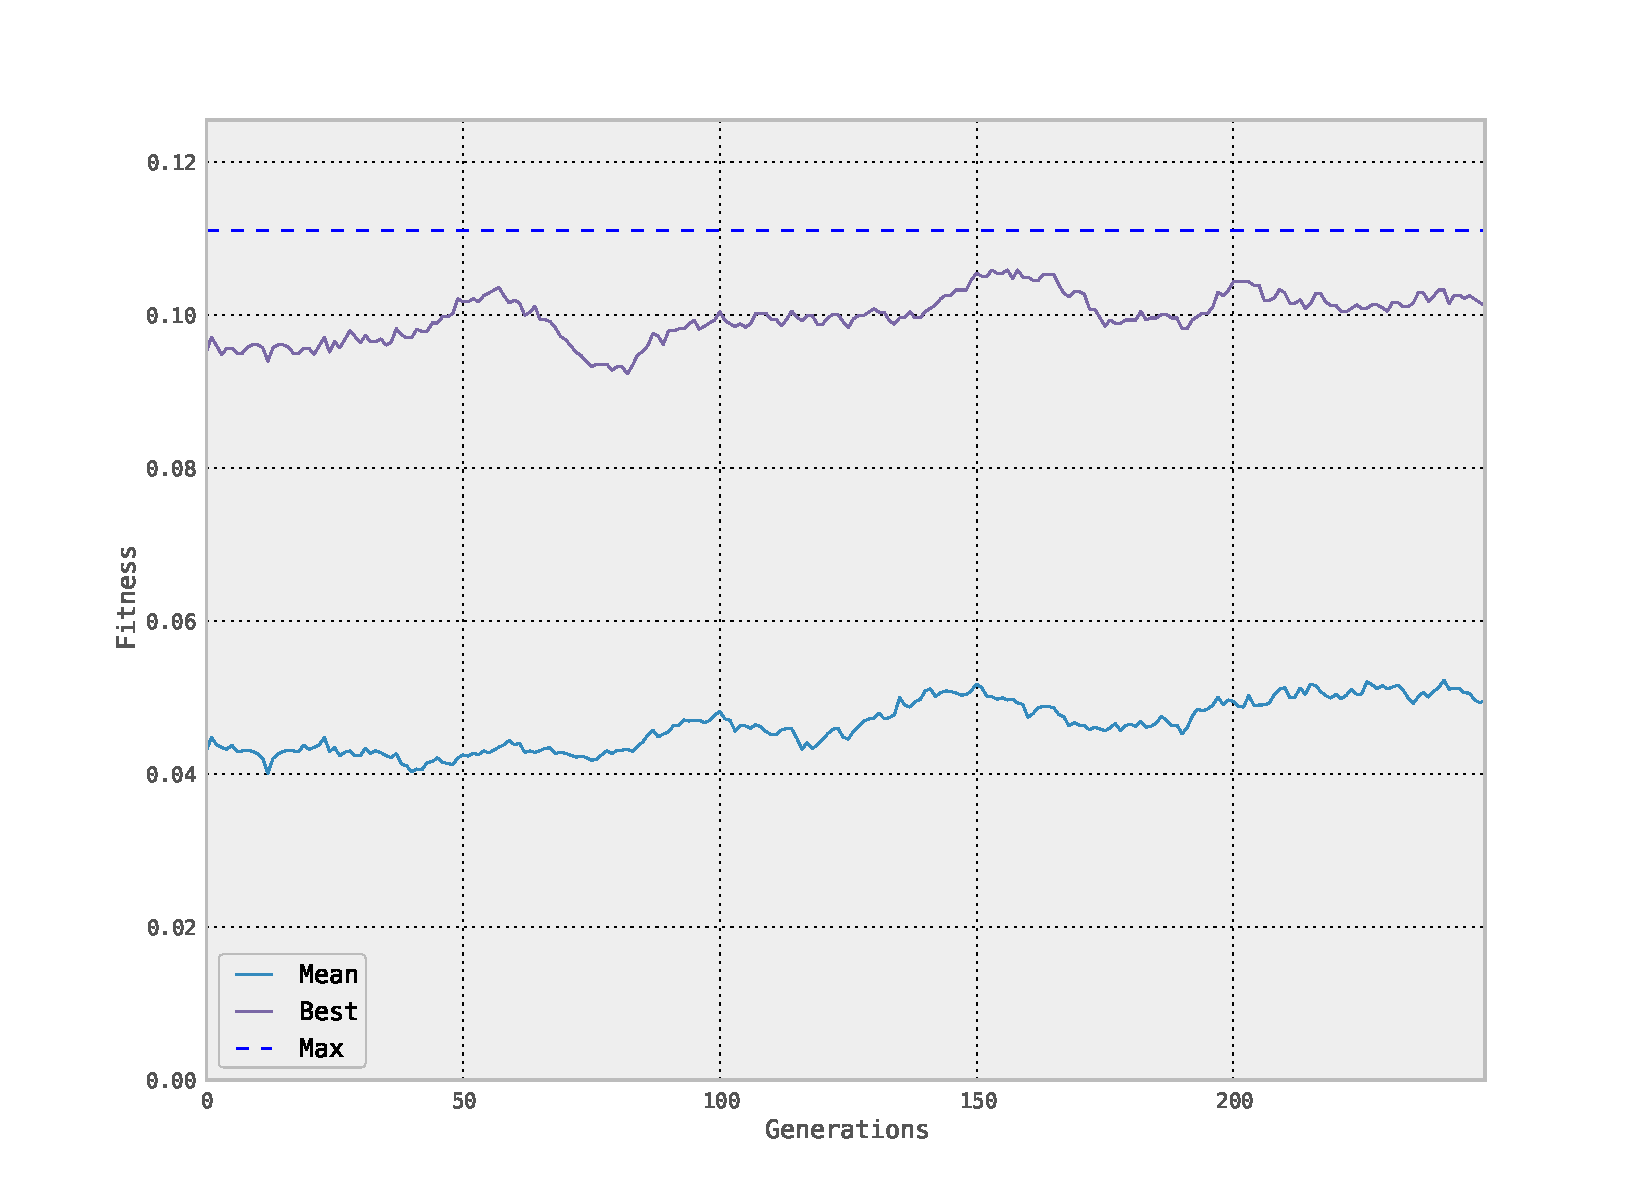
\includegraphics[scale =0.4] {images/section3/fitness_1_10_001.pdf}
	\label{fig:figure23}
}
\subfigure[Pheromones per edge]{
	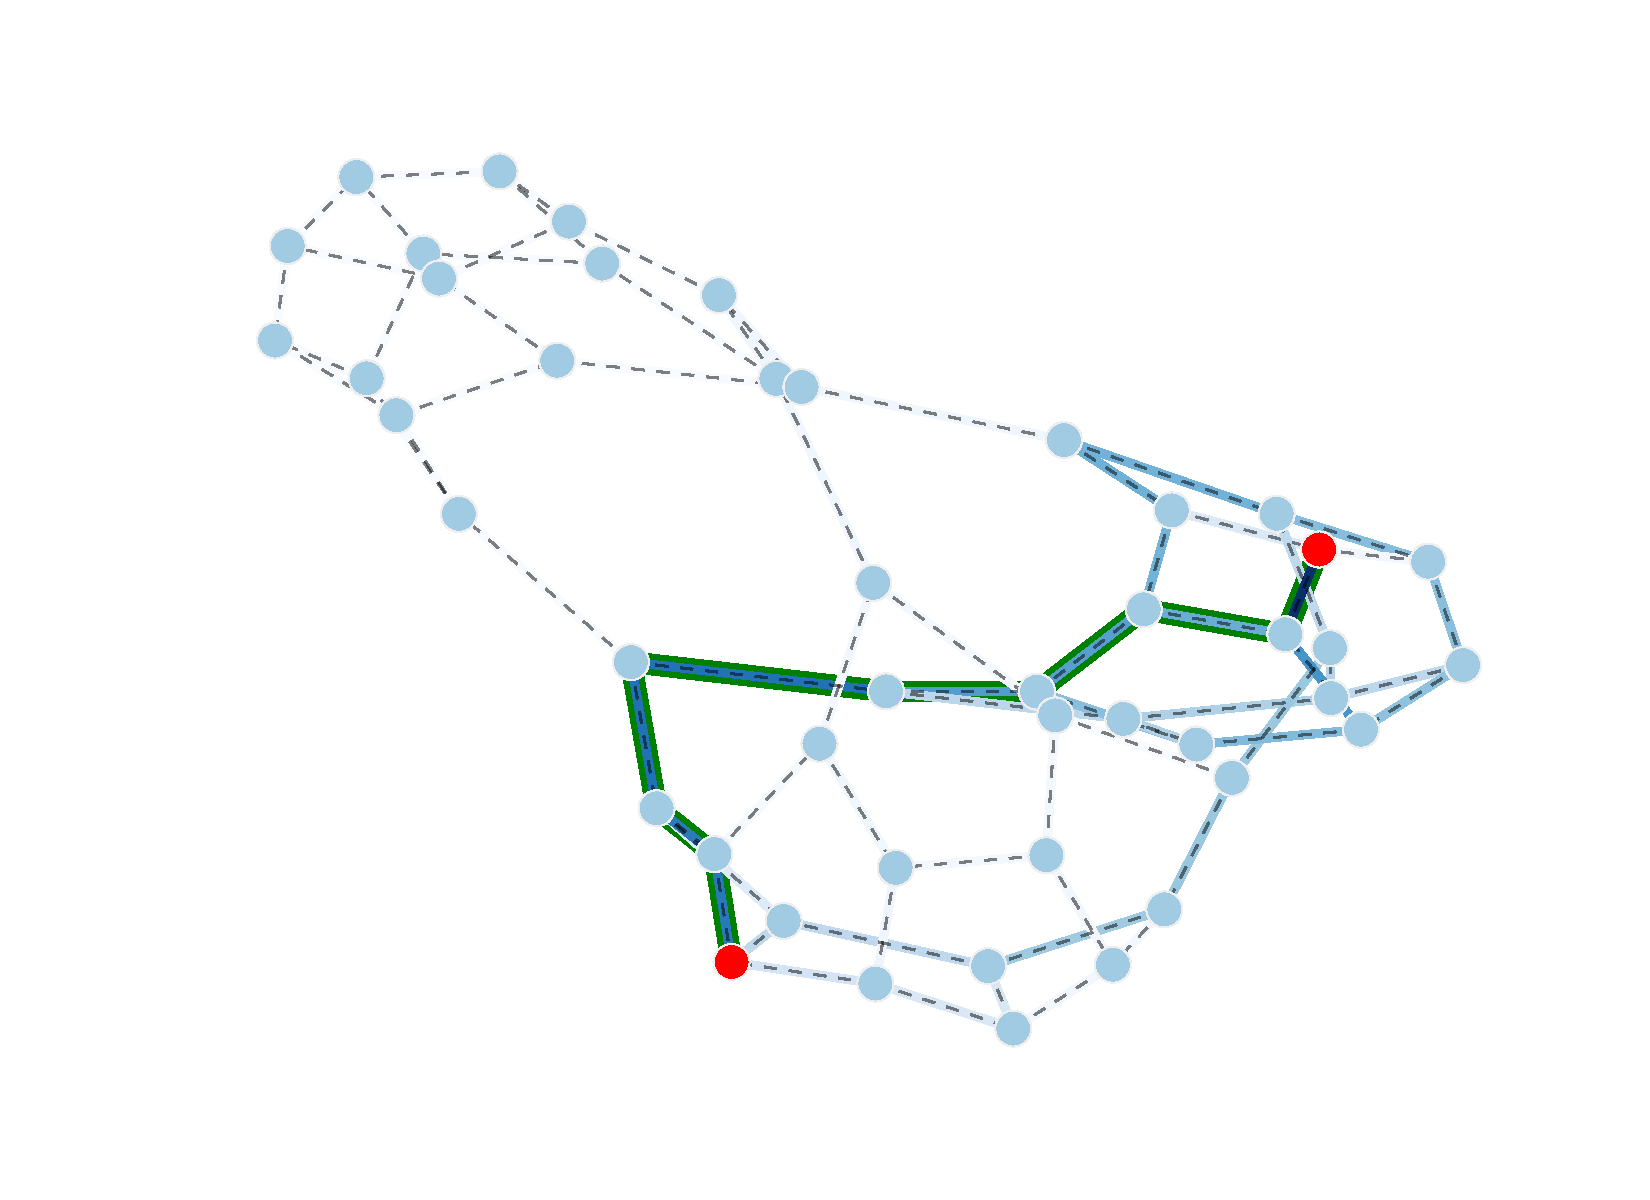
\includegraphics[scale =0.4] {images/section3/pheromones_10_001.pdf}
	\label{fig:figure22}
}
%\caption[Optional caption for list of figures]{Caption of subfigures \subref{fig:subfig1}, \subref{fig:subfig2}}
\label{fig:figure2}
\end{figure}





\newpage
\subsection{Set $\rho = 0.1, k=15$}

\begin{figure}[ht]
\centering
\subfigure[Fitness evolution]{
	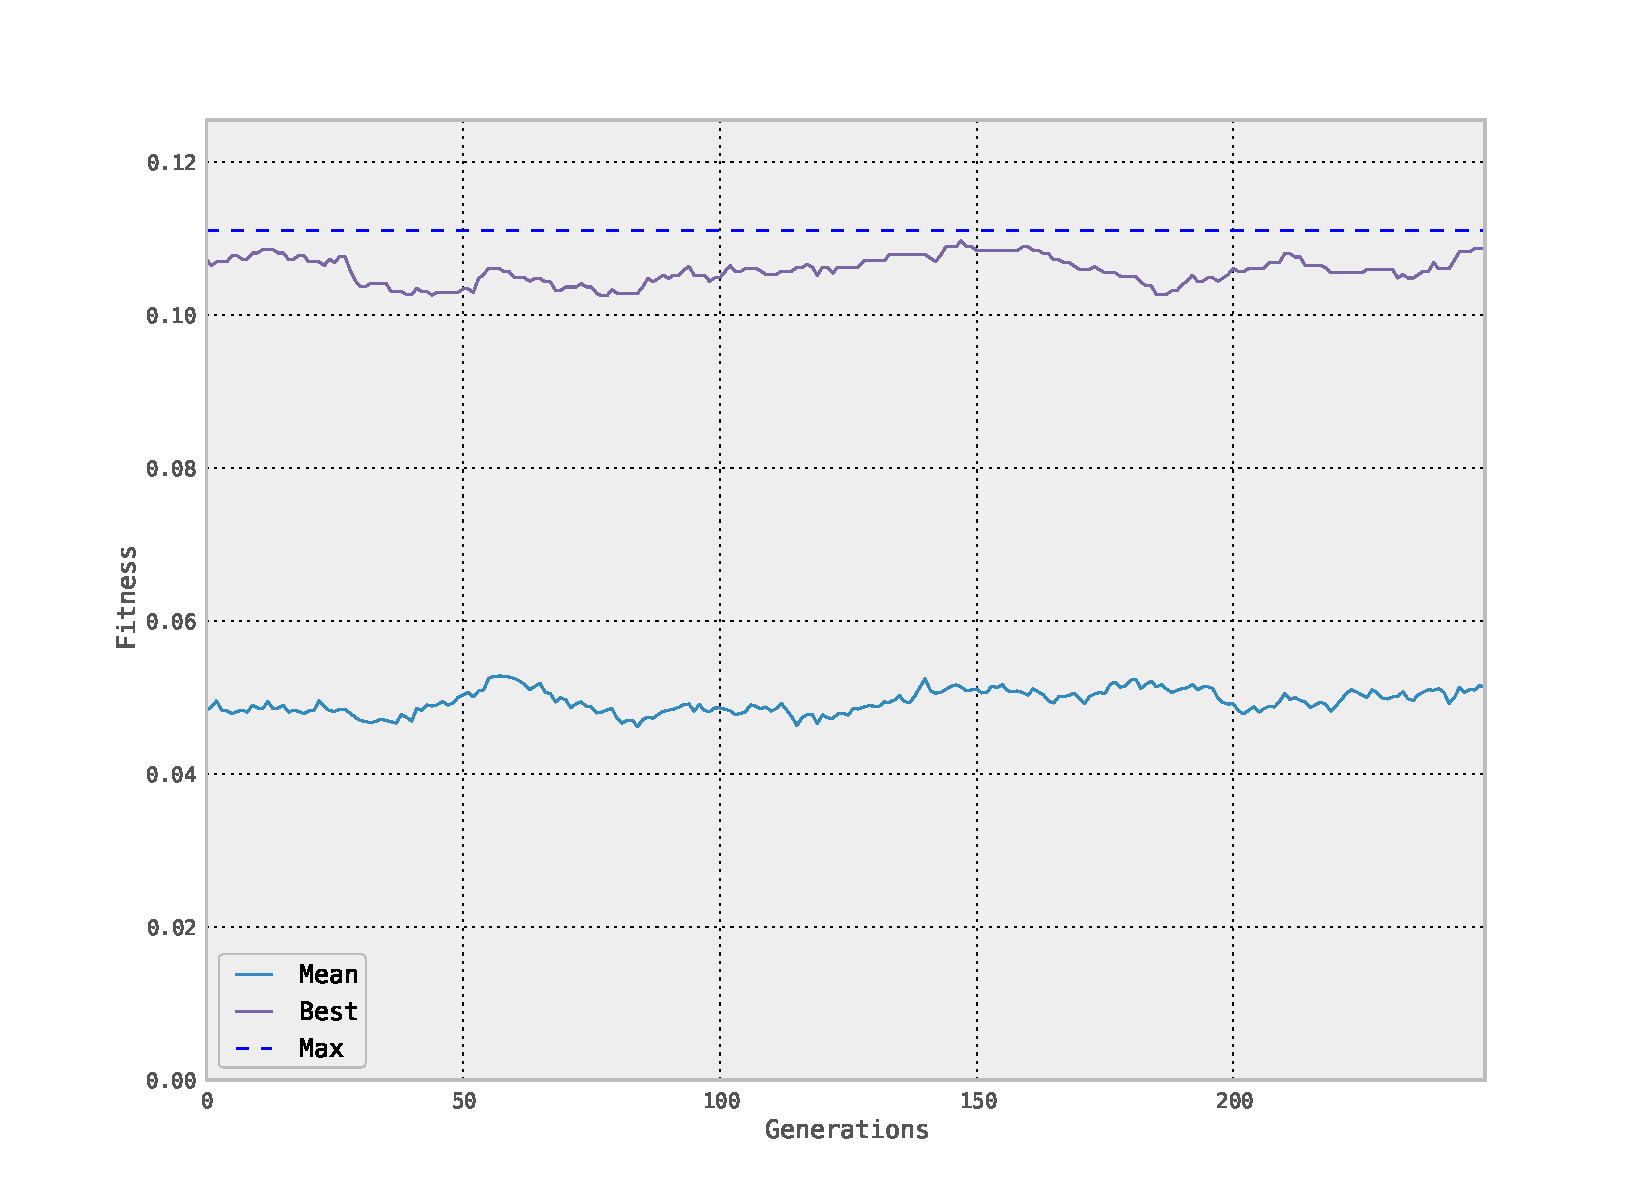
\includegraphics[scale =0.4] {images/section3/fitness_1_15_001.pdf}
	\label{fig:figure31}
}
\subfigure[Pheromones per edge]{
	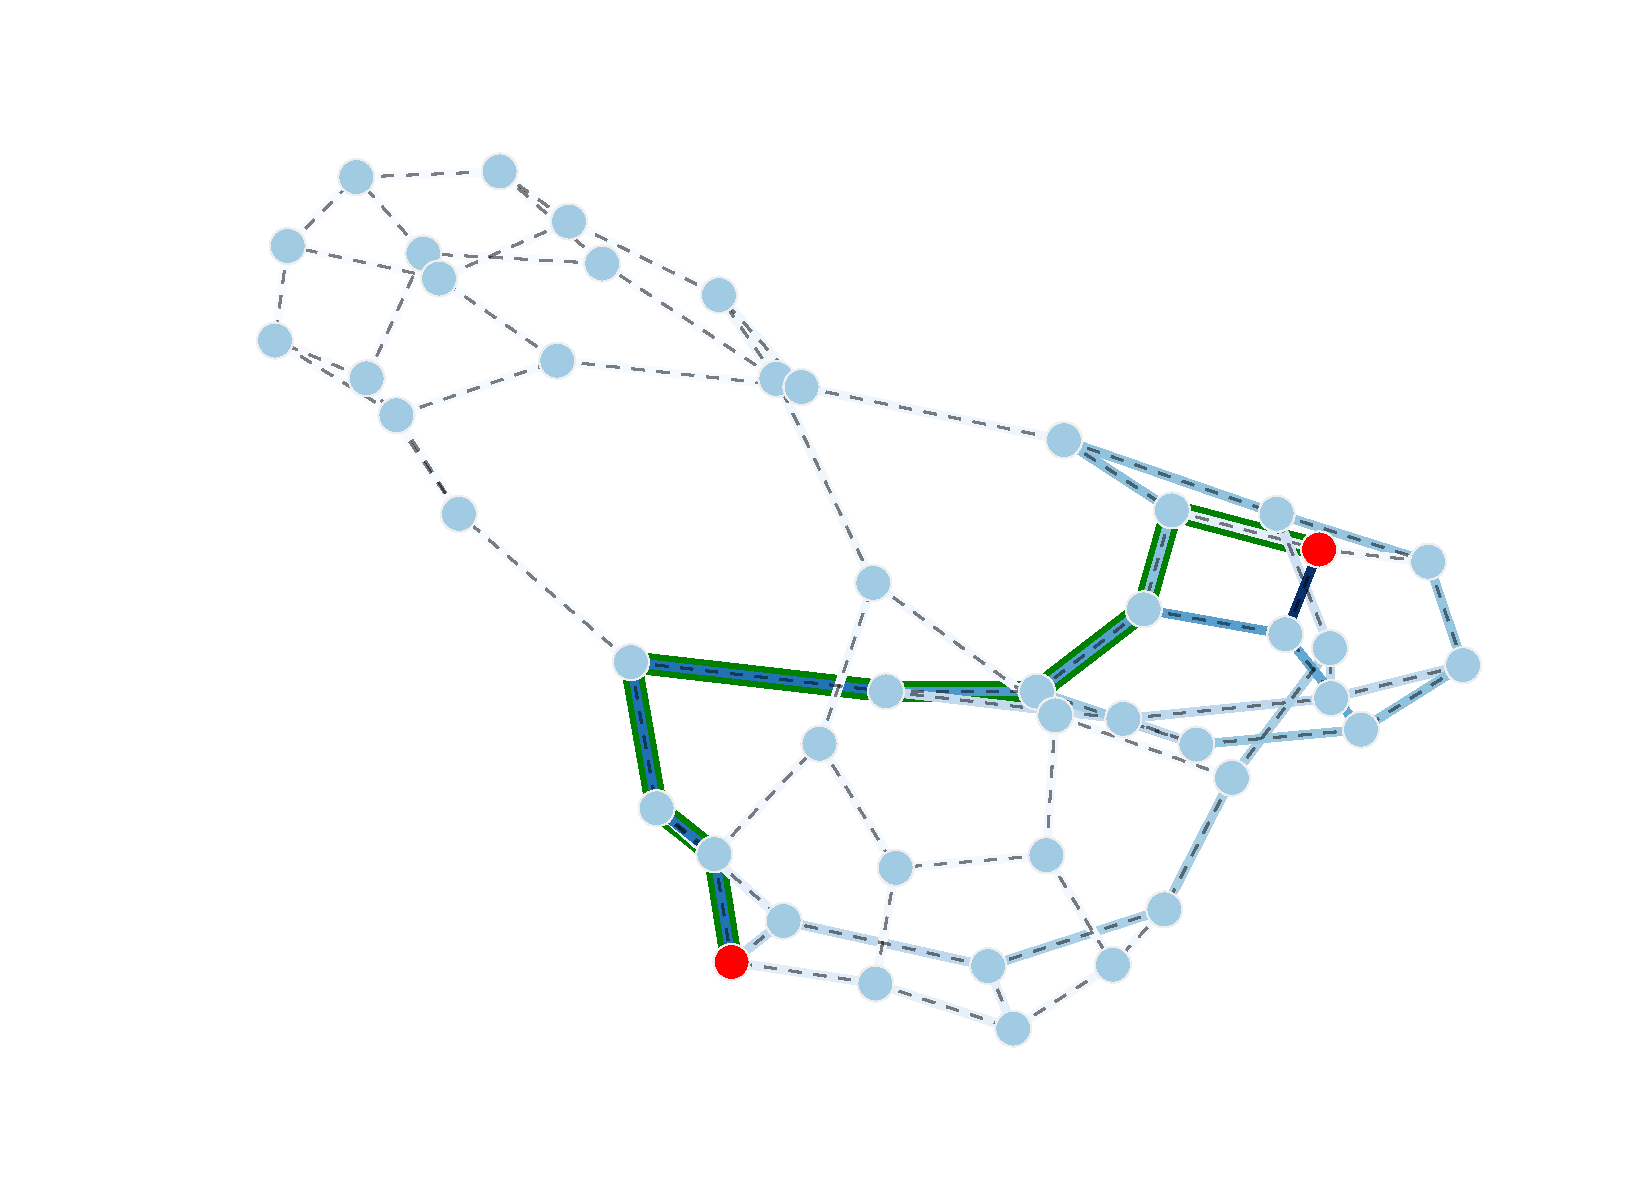
\includegraphics[scale =0.4] {images/section3/pheromones_15_001.pdf}
	\label{fig:figure32}
}
%\caption[Optional caption for list of figures]{Caption of subfigures \subref{fig:subfig1}, \subref{fig:subfig2}}
\label{fig:figure3}
\end{figure}


\newpage
\subsection{Set $\rho = 0.1, k=50$}

\begin{figure}[ht]
\centering
\subfigure[Fitness evolution]{
	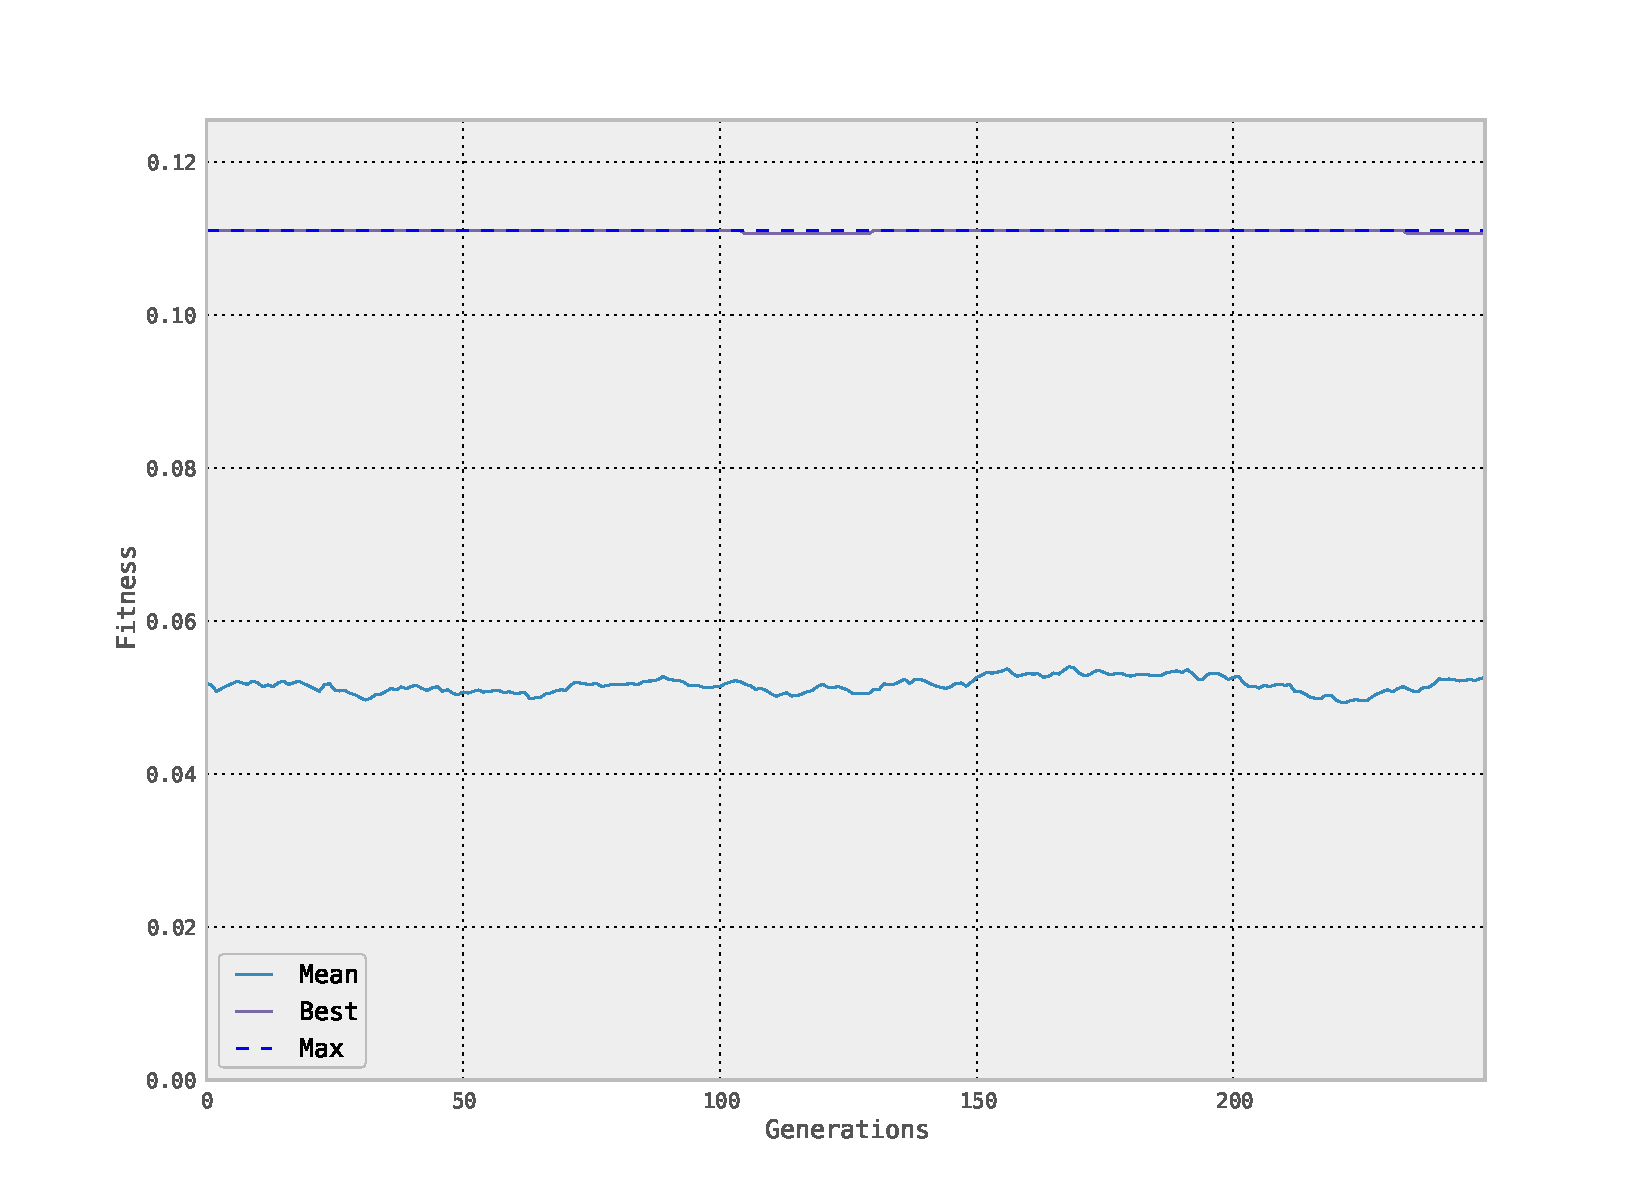
\includegraphics[scale =0.4] {images/section3/fitness_1_50_001.pdf}
	\label{fig:figure41}
}
\subfigure[Pheromones per edge]{
	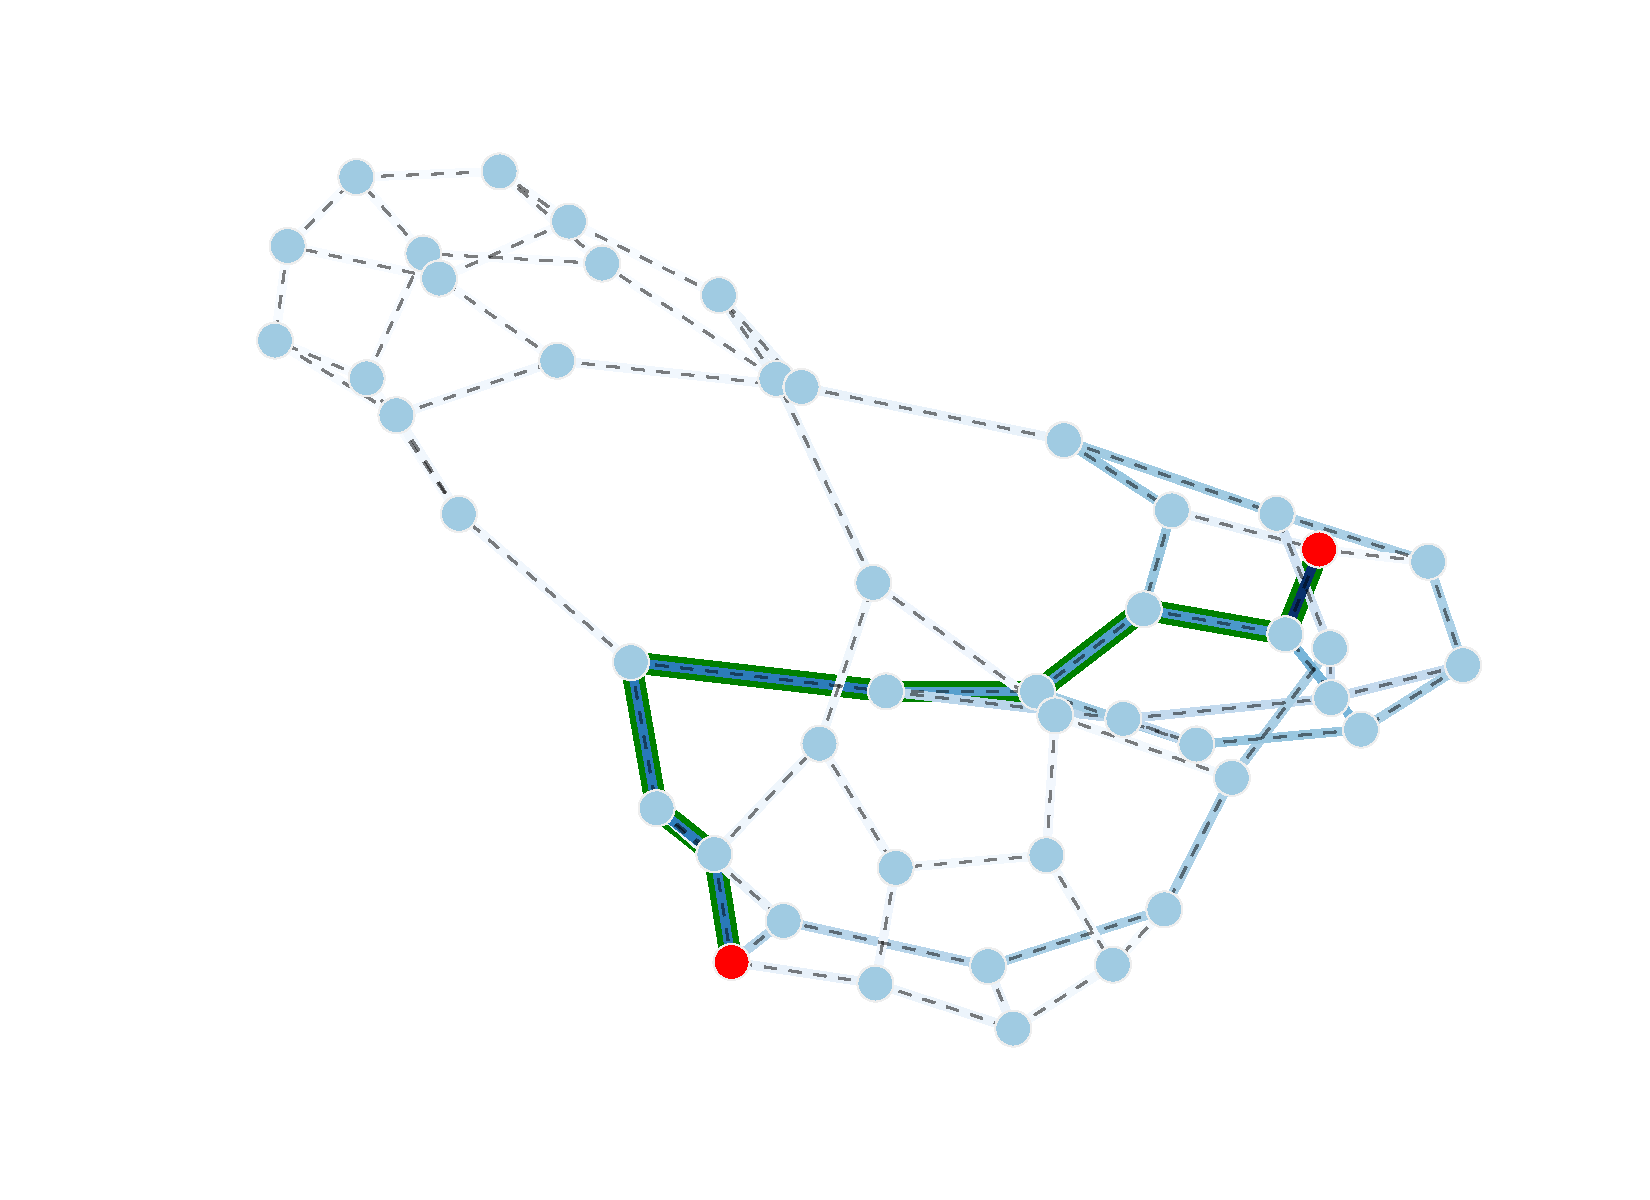
\includegraphics[scale =0.4] {images/section3/pheromones_50_001.pdf}
	\label{fig:figure42}
}
%\caption[Optional caption for list of figures]{Caption of subfigures \subref{fig:subfig1}, \subref{fig:subfig2}}
\label{fig:figure4}
\end{figure}




\newpage
\subsection{Set $\rho = 0.1, k=100$}

\begin{figure}[ht]
\centering
\subfigure[Fitness evolution]{
	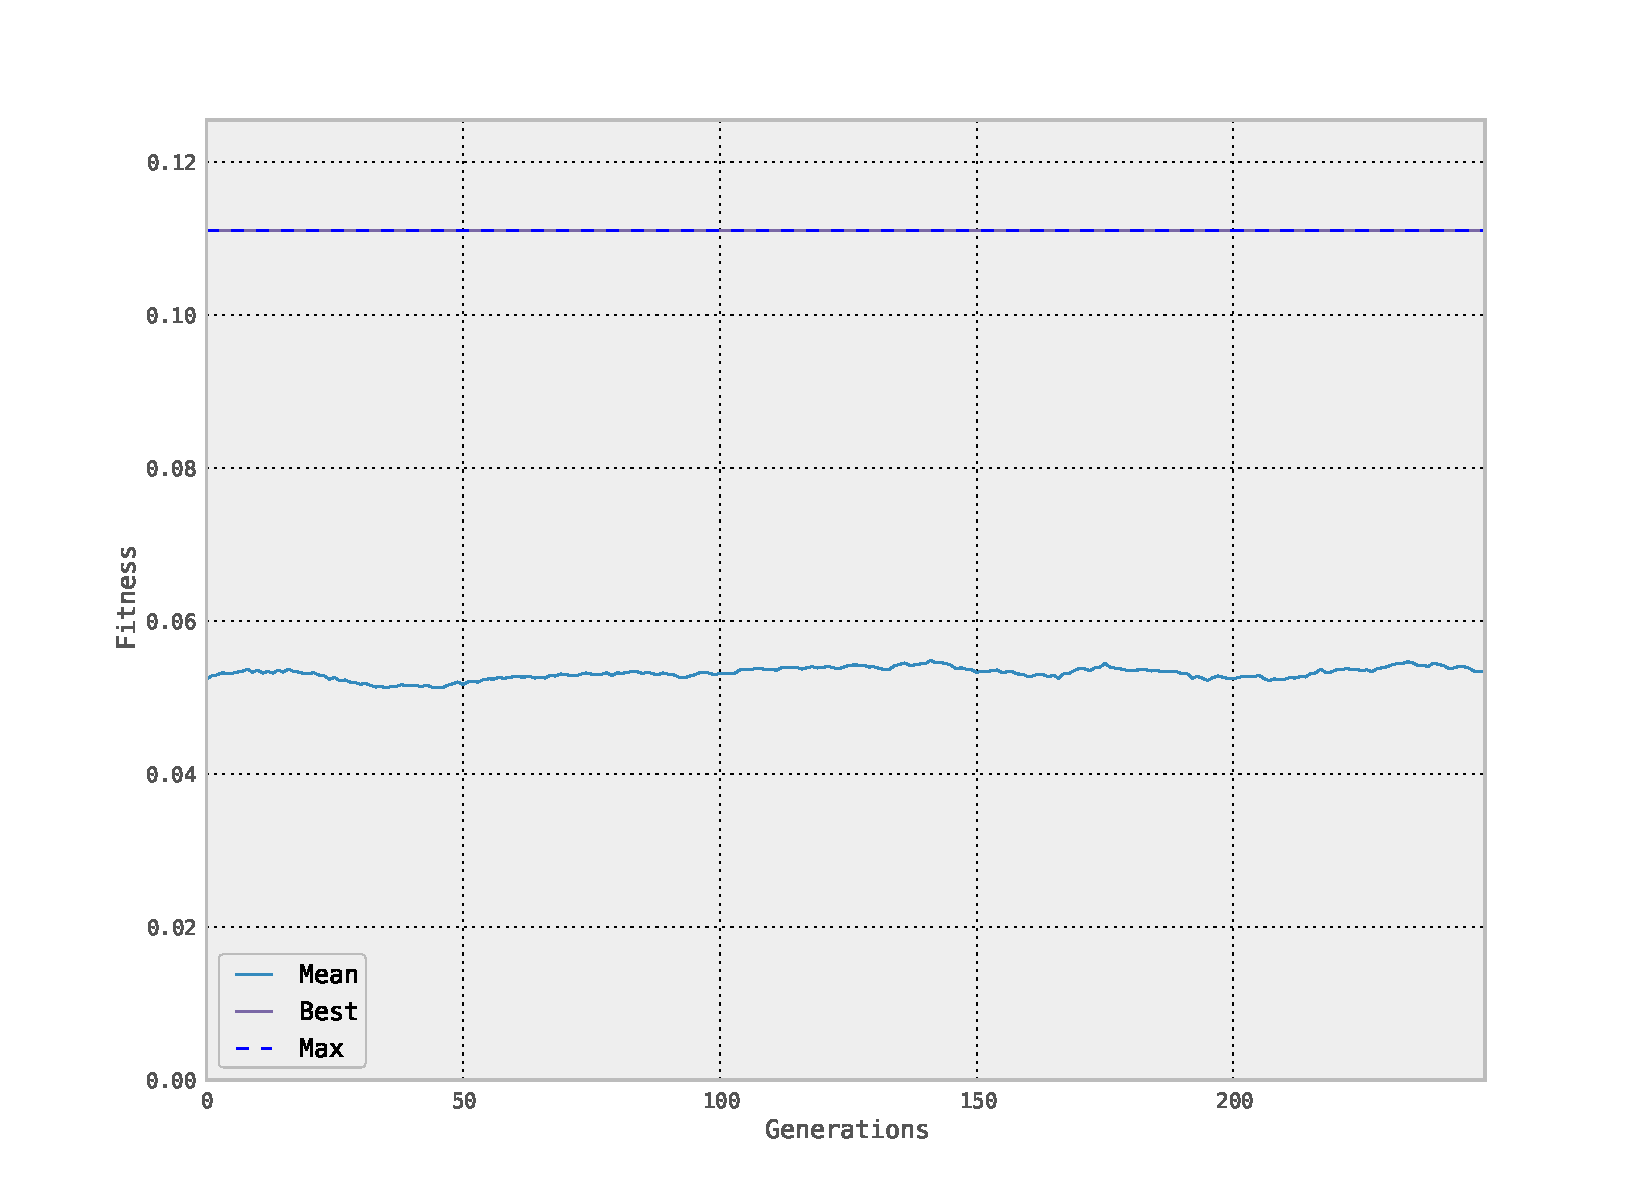
\includegraphics[scale =0.4] {images/section3/fitness_1_100_001.pdf}
	\label{fig:figure51}
}
\subfigure[Pheromones per edge]{
	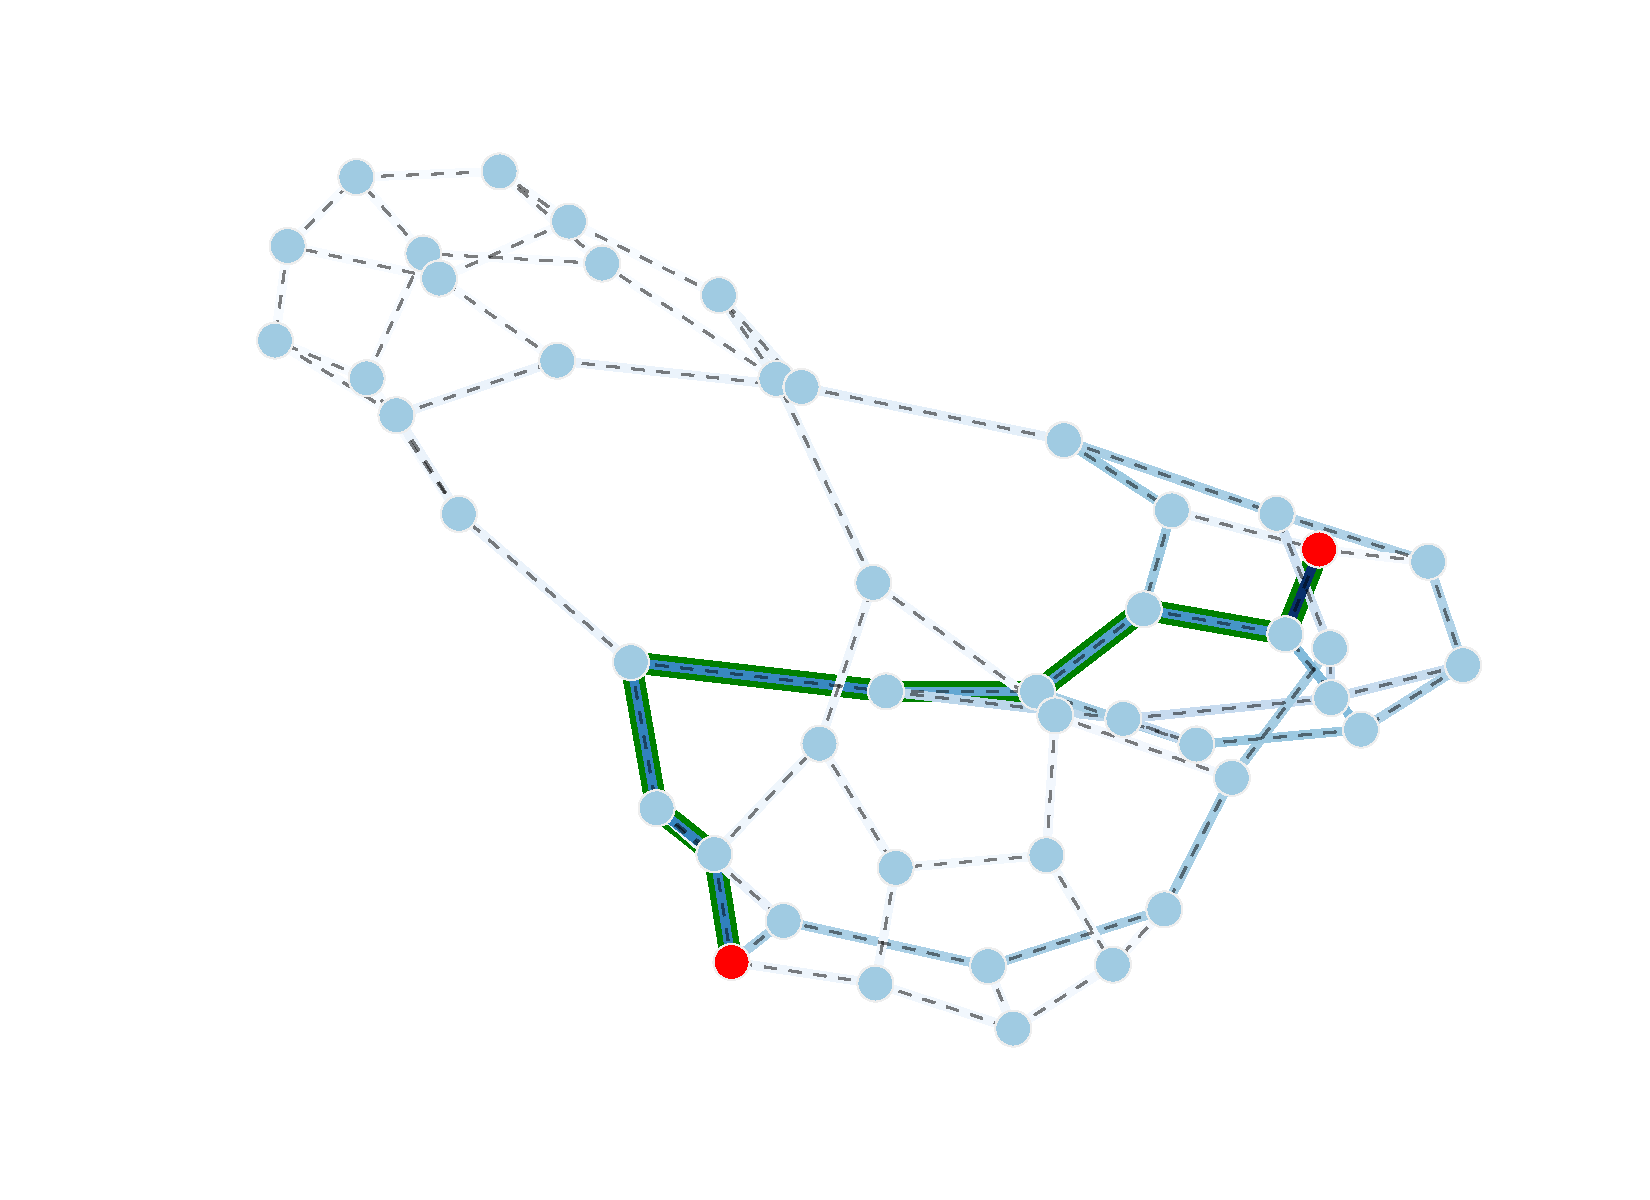
\includegraphics[scale =0.4] {images/section3/pheromones_100_001.pdf}
	\label{fig:figure52}
}
%\caption[Optional caption for list of figures]{Caption of subfigures \subref{fig:subfig1}, \subref{fig:subfig2}}
\label{fig:figure5}
\end{figure}





\newpage
\subsection{Set $\rho = 0.5, k=5$}

\begin{figure}[ht]
\centering
\subfigure[Fitness evolution]{
	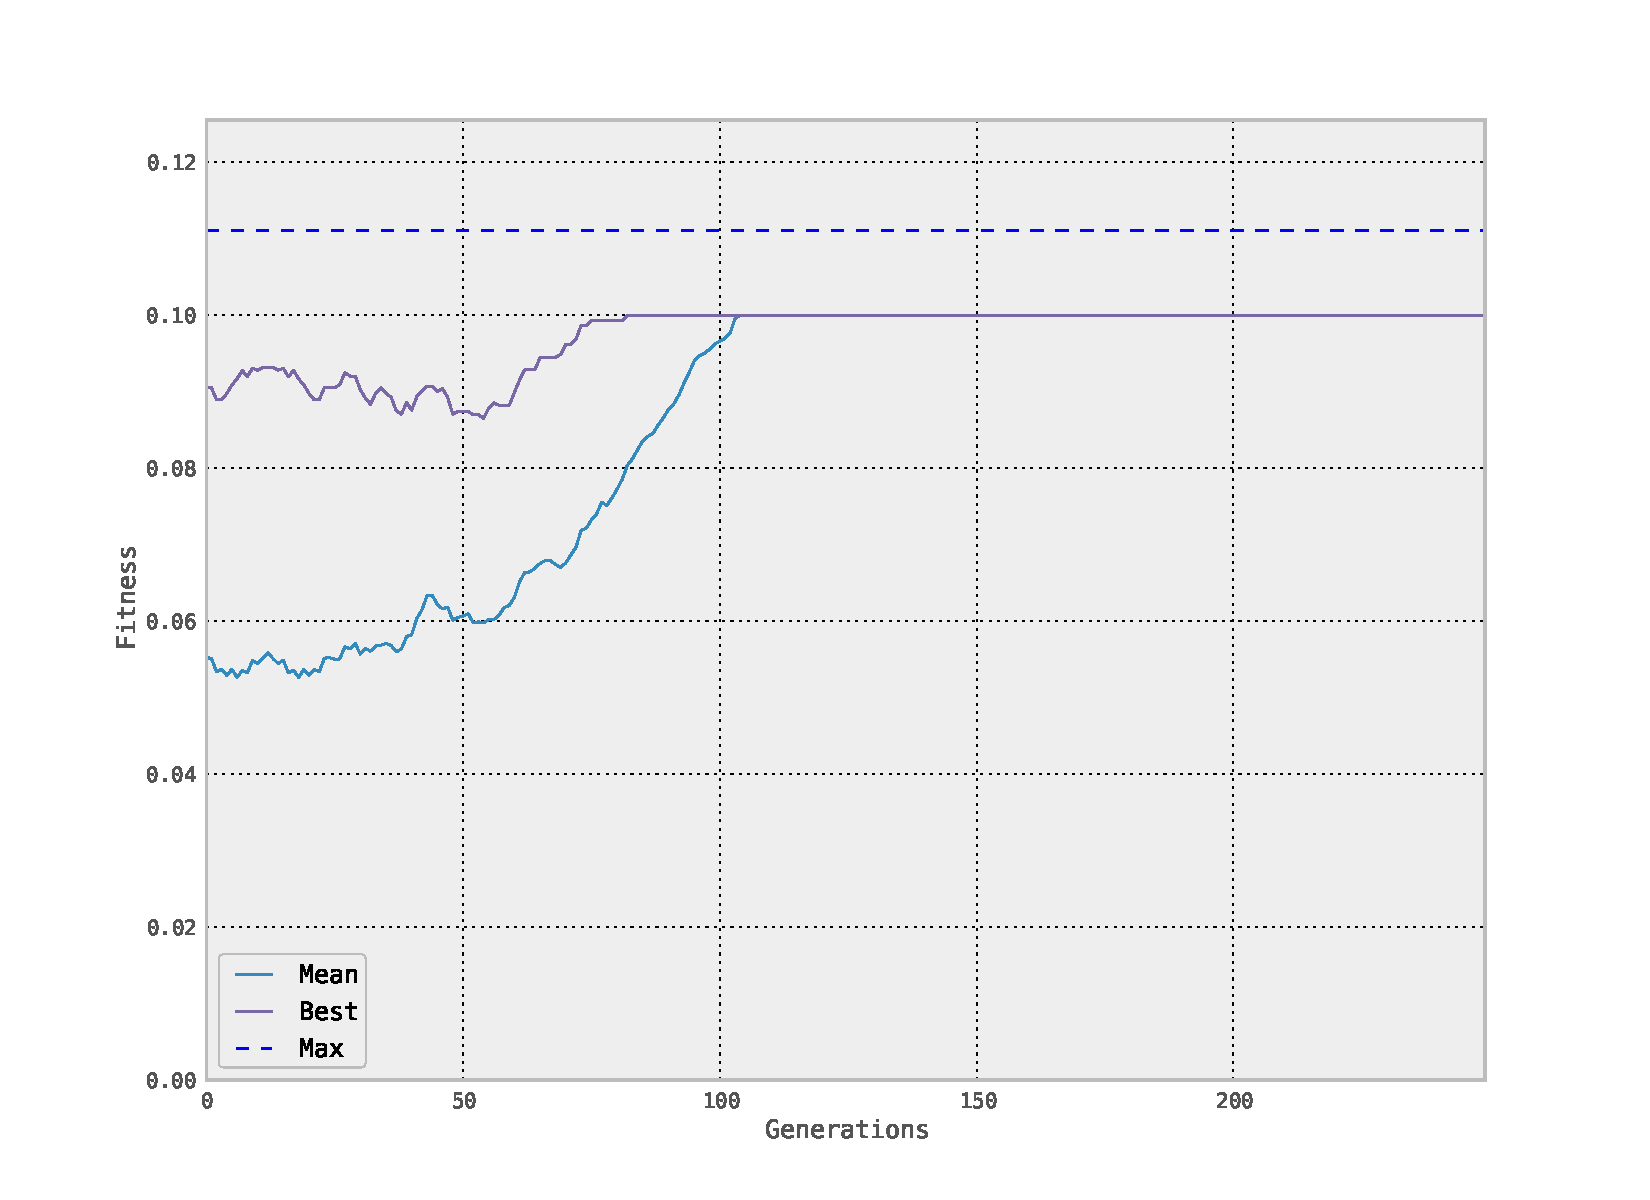
\includegraphics[scale =0.4] {images/section3/fitness_1_5_05.pdf}
	\label{fig:figure61}
}
\subfigure[Pheromones per edge]{
	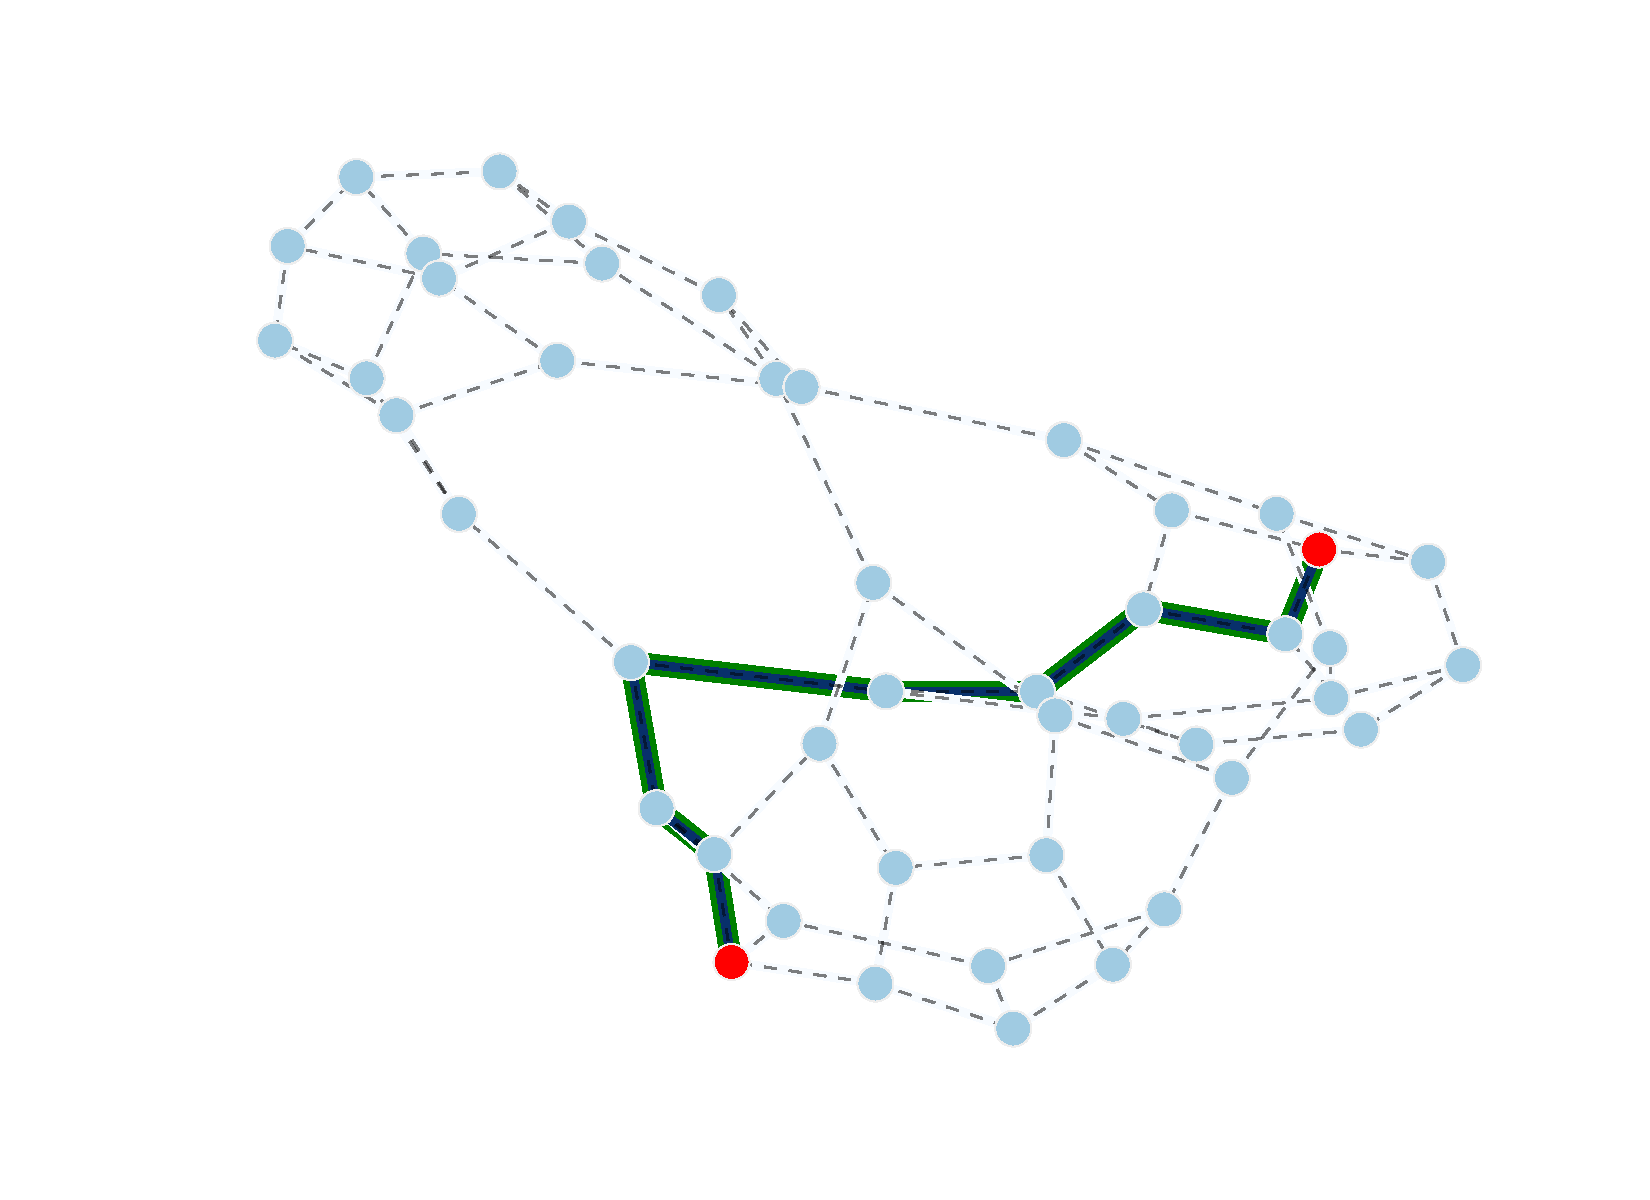
\includegraphics[scale =0.4] {images/section3/pheromones_5_05.pdf}
	\label{fig:figure62}
}
%\caption[Optional caption for list of figures]{Caption of subfigures \subref{fig:subfig1}, \subref{fig:subfig2}}
\label{fig:figure6}
\end{figure}






\newpage
\subsection{Set $\rho = 0.5, k=10$}

\begin{figure}[ht]
\centering
\subfigure[Fitness evolution]{
	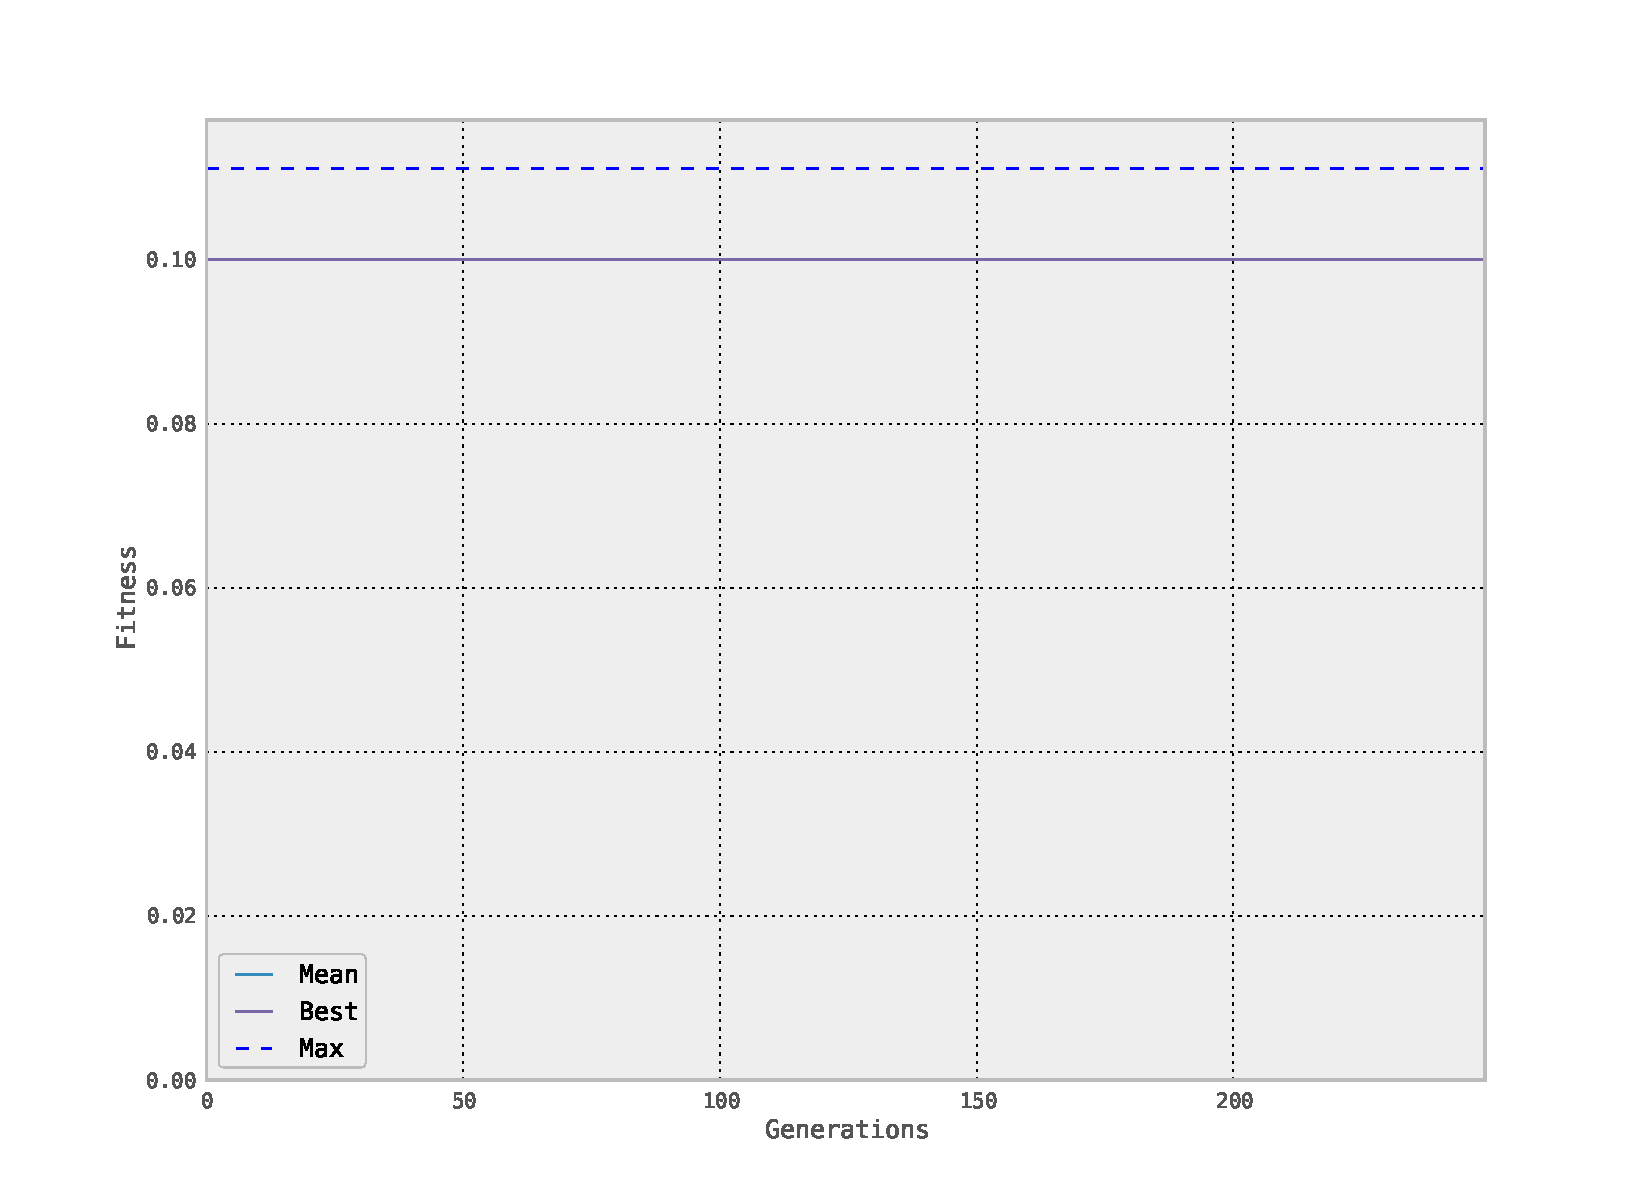
\includegraphics[scale =0.4] {images/section3/fitness_1_10_05.pdf}
	\label{fig:figure71}
}
\subfigure[Pheromones per edge]{
	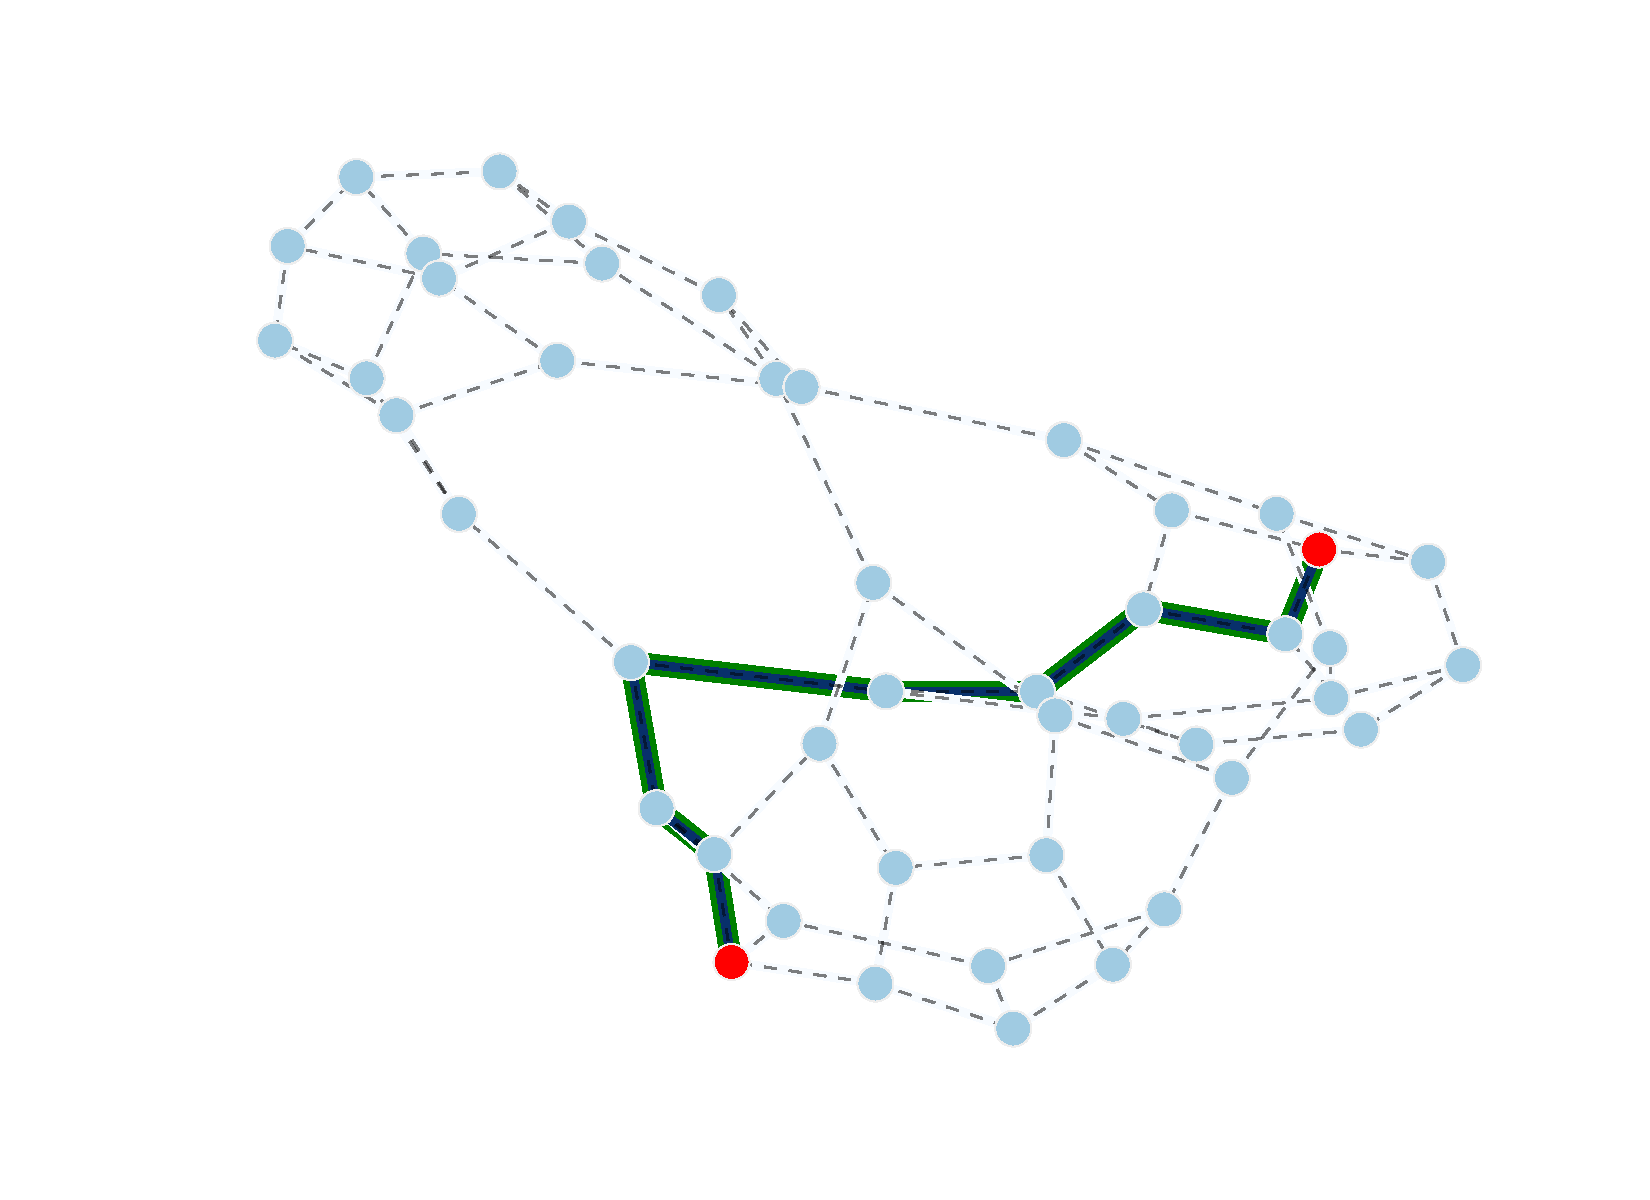
\includegraphics[scale =0.4] {images/section3/pheromones_10_05.pdf}
	\label{fig:figure72}
}
%\caption[Optional caption for list of figures]{Caption of subfigures \subref{fig:subfig1}, \subref{fig:subfig2}}
\label{fig:figure7}
\end{figure}





\newpage
\subsection{Set $\rho = 0.5, k=15$}

\begin{figure}[ht]
\centering
\subfigure[Fitness evolution]{
	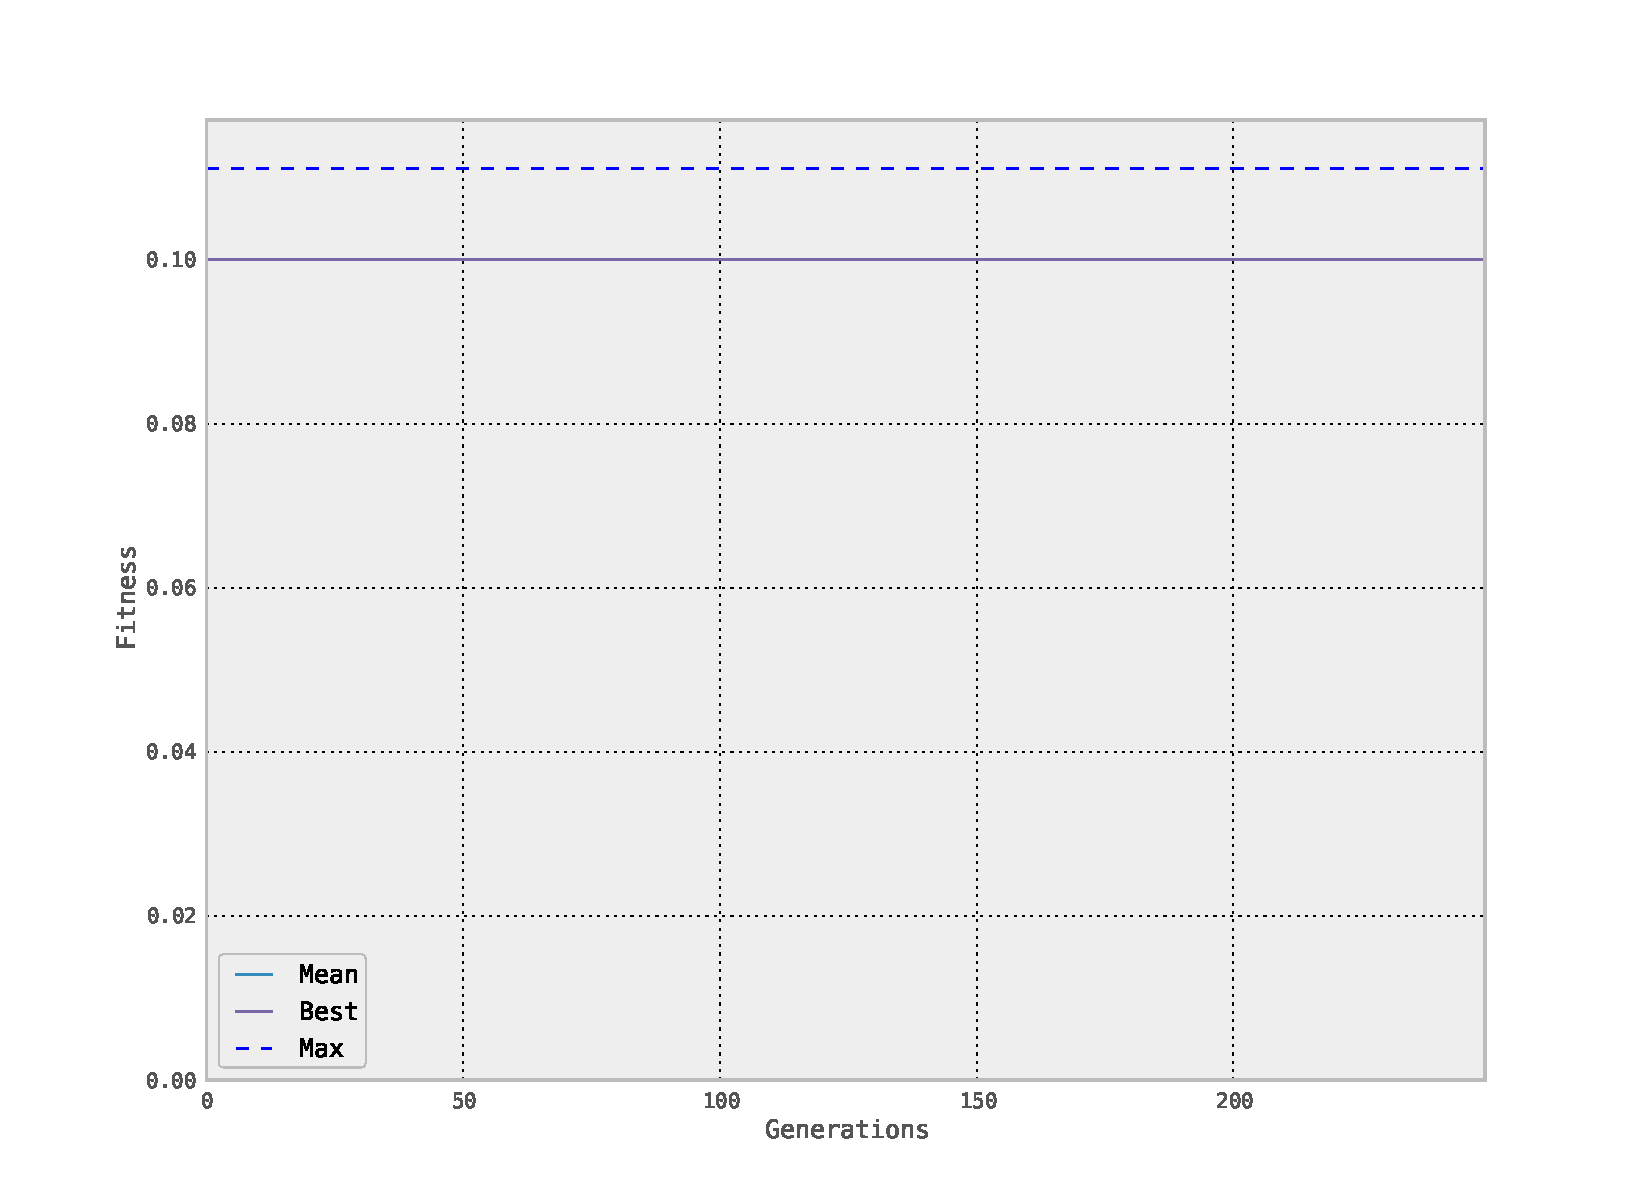
\includegraphics[scale =0.4] {images/section3/fitness_1_15_05.pdf}
	\label{fig:figure81}
}
\subfigure[Pheromones per edge]{
	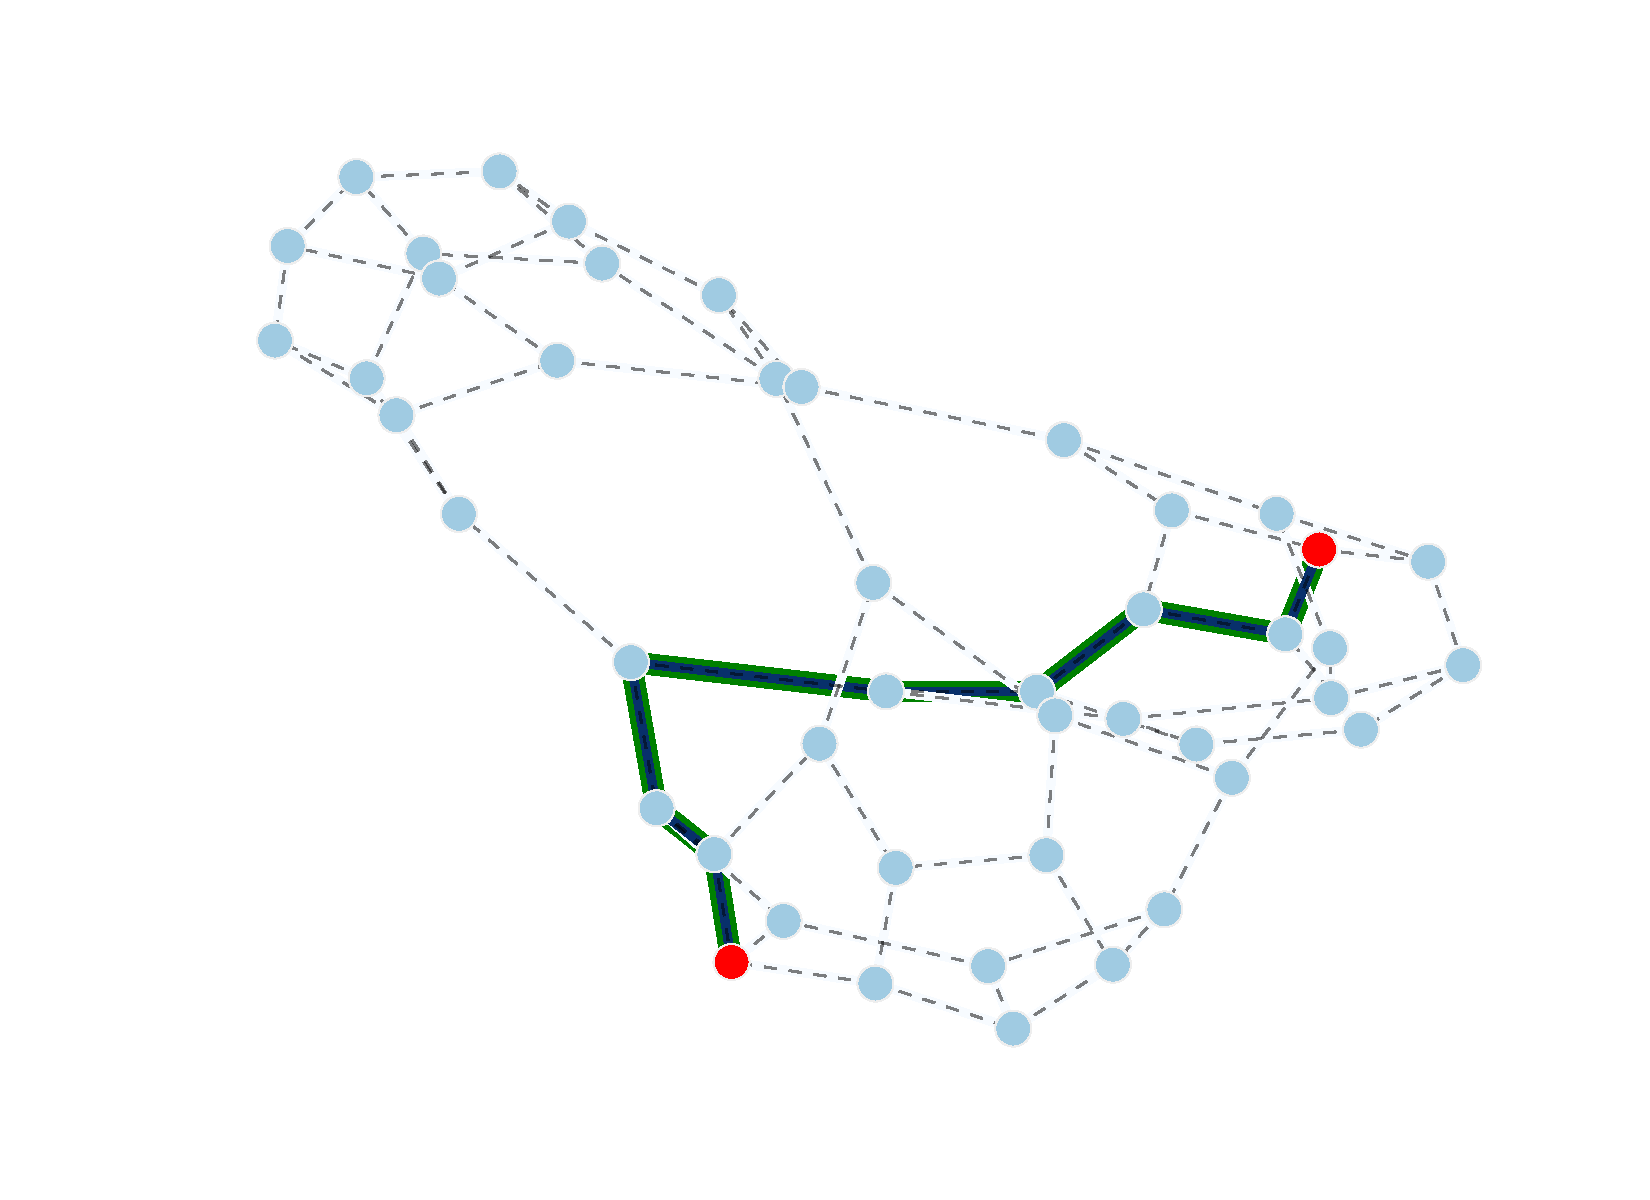
\includegraphics[scale =0.4] {images/section3/pheromones_15_05.pdf}
	\label{fig:figure82}
}
%\caption[Optional caption for list of figures]{Caption of subfigures \subref{fig:subfig1}, \subref{fig:subfig2}}
\label{fig:figure8}
\end{figure}





\newpage
\subsection{Set $\rho = 0.5, k=50$}



\begin{figure}[ht]
\centering
\subfigure[Fitness evolution]{
	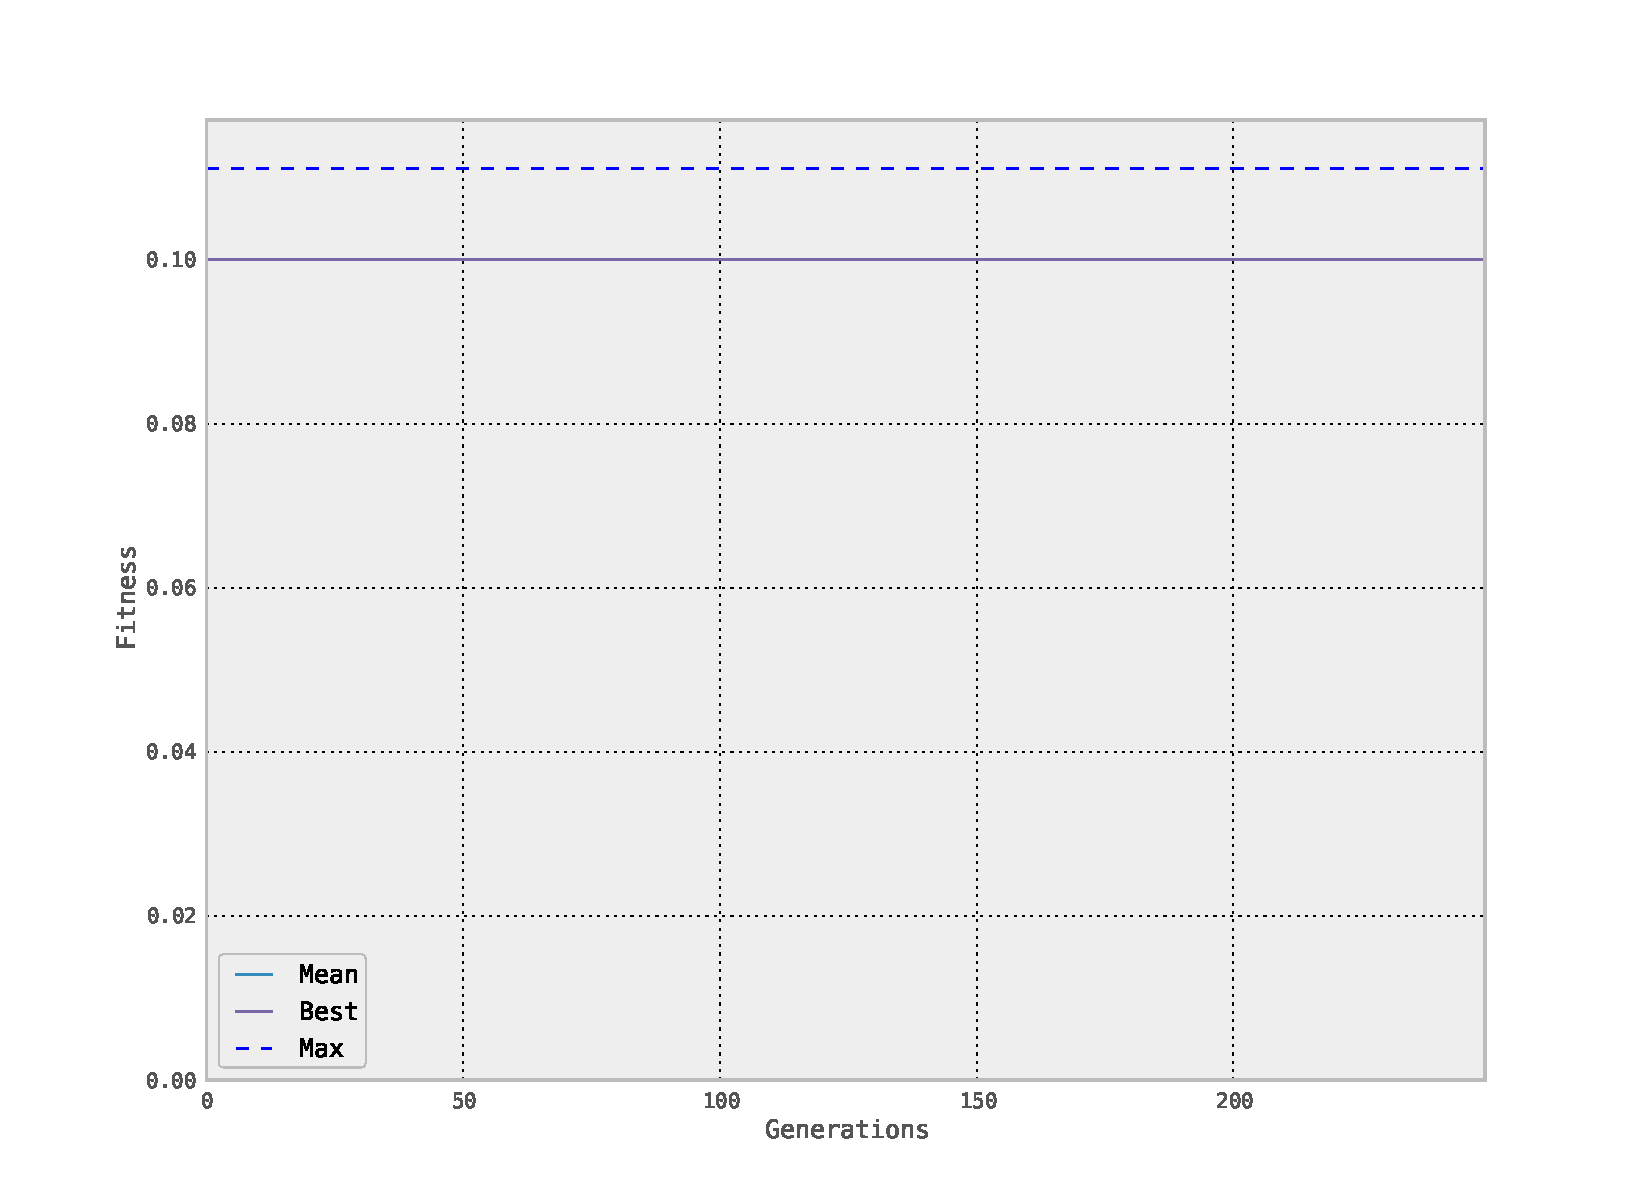
\includegraphics[scale =0.4] {images/section3/fitness_1_50_05.pdf}
	\label{fig:figure91}
}
\subfigure[Pheromones per edge]{
	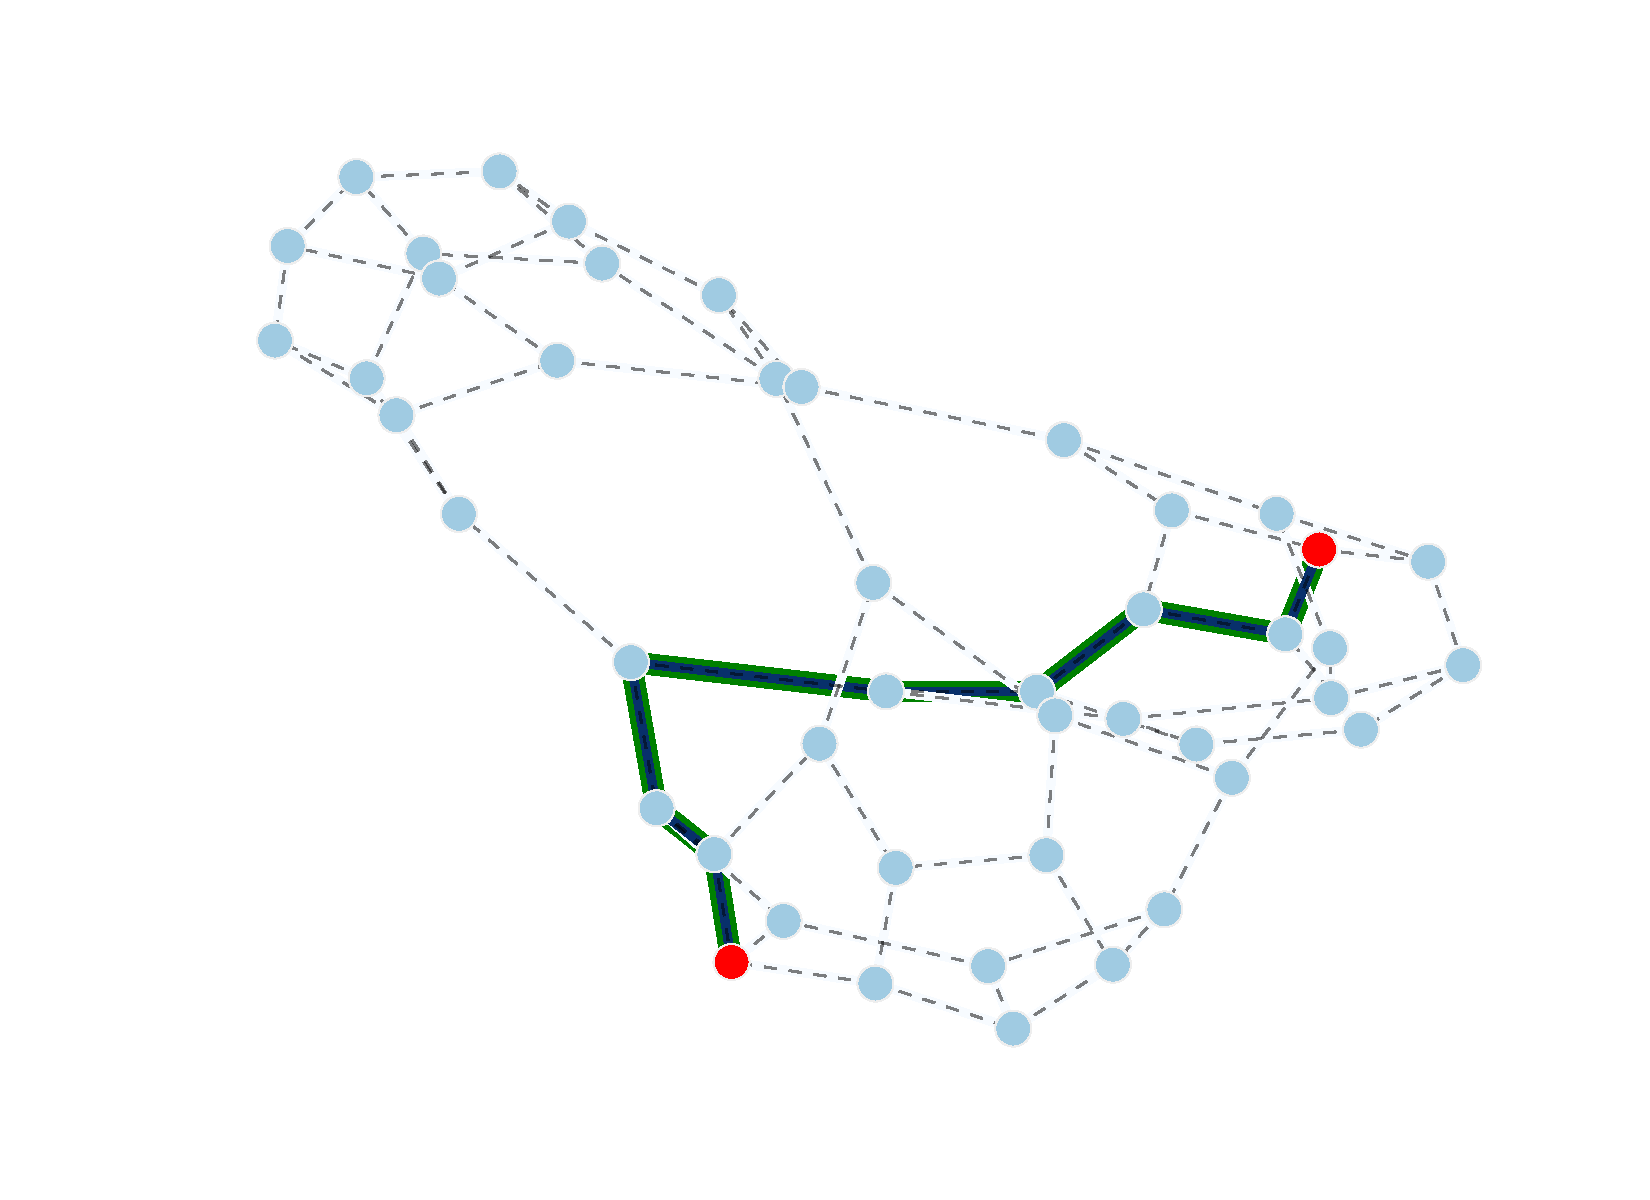
\includegraphics[scale =0.4] {images/section3/pheromones_50_05.pdf}
	\label{fig:figure92}
}
%\caption[Optional caption for list of figures]{Caption of subfigures \subref{fig:subfig1}, \subref{fig:subfig2}}
\label{fig:figure9}
\end{figure}



\newpage
\subsection{Set $\rho = 0.5, k=100$}


\begin{figure}[ht]
\centering
\subfigure[Fitness evolution]{
	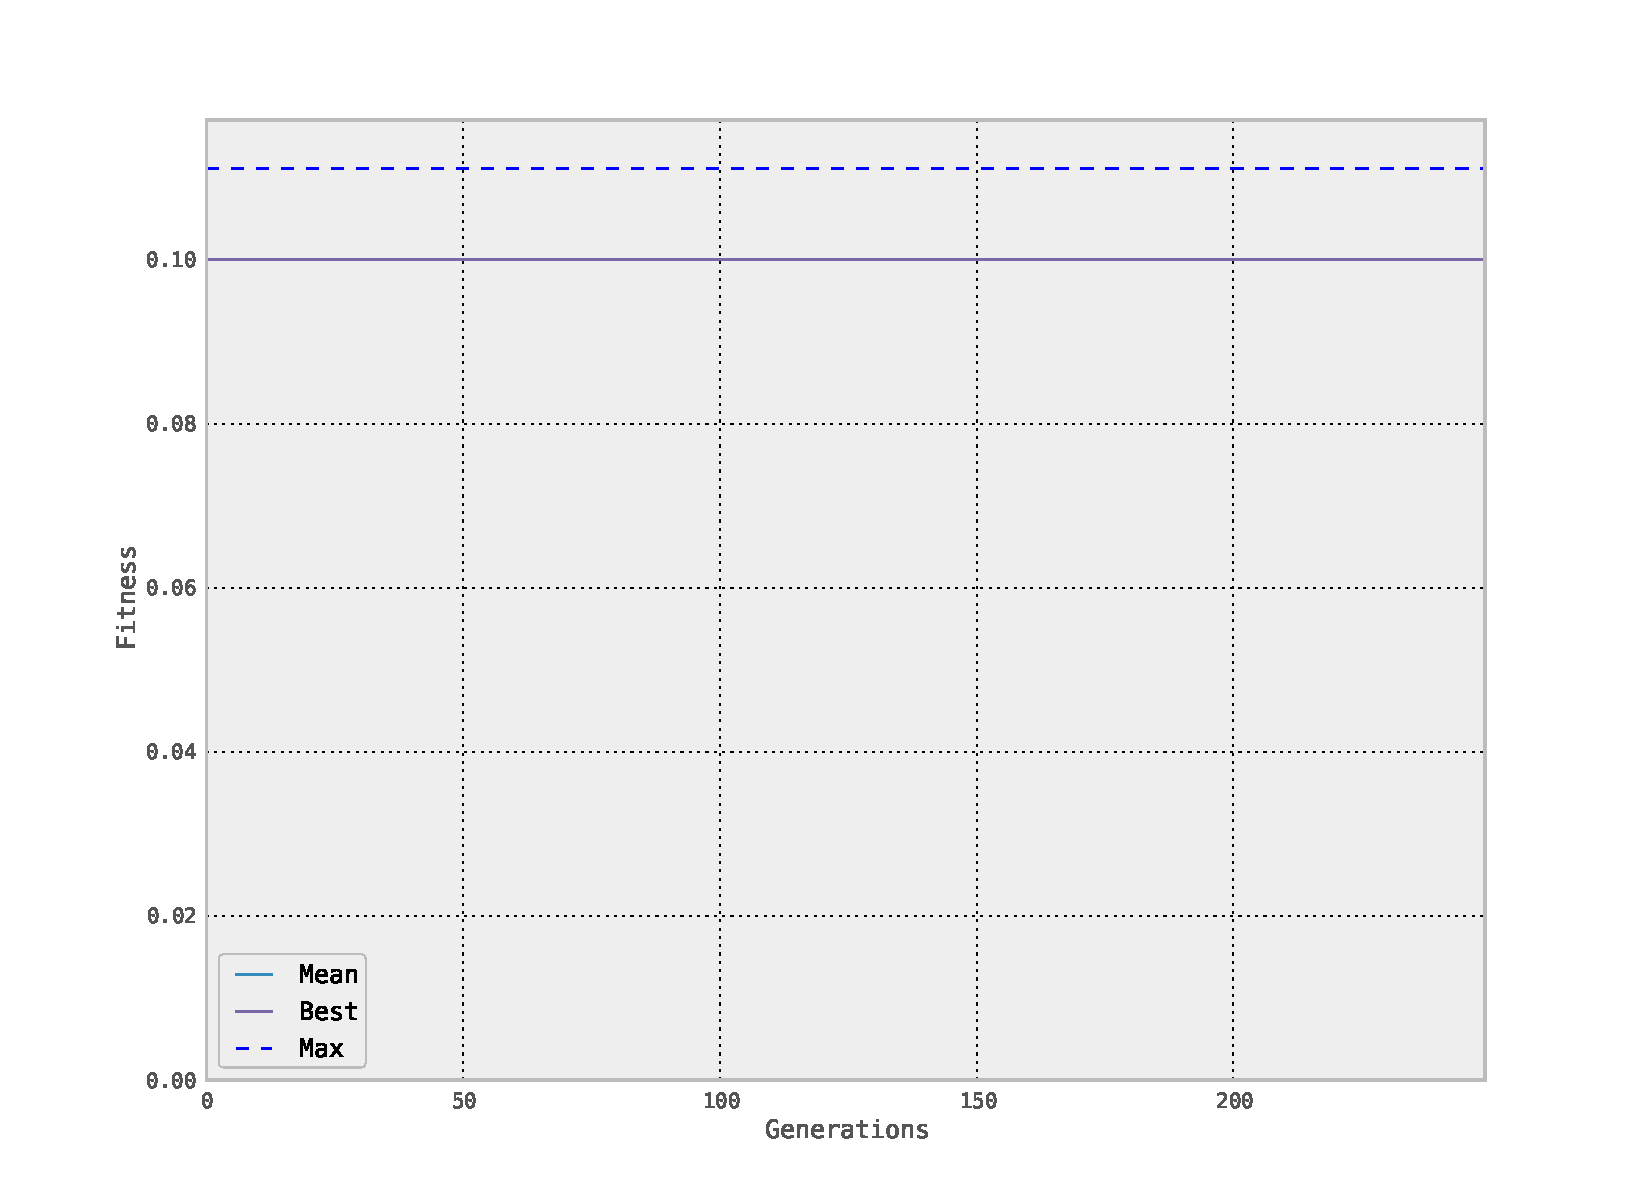
\includegraphics[scale =0.4] {images/section3/fitness_1_100_05.pdf}
	\label{fig:figure101}
}
\subfigure[Pheromones per edge]{
	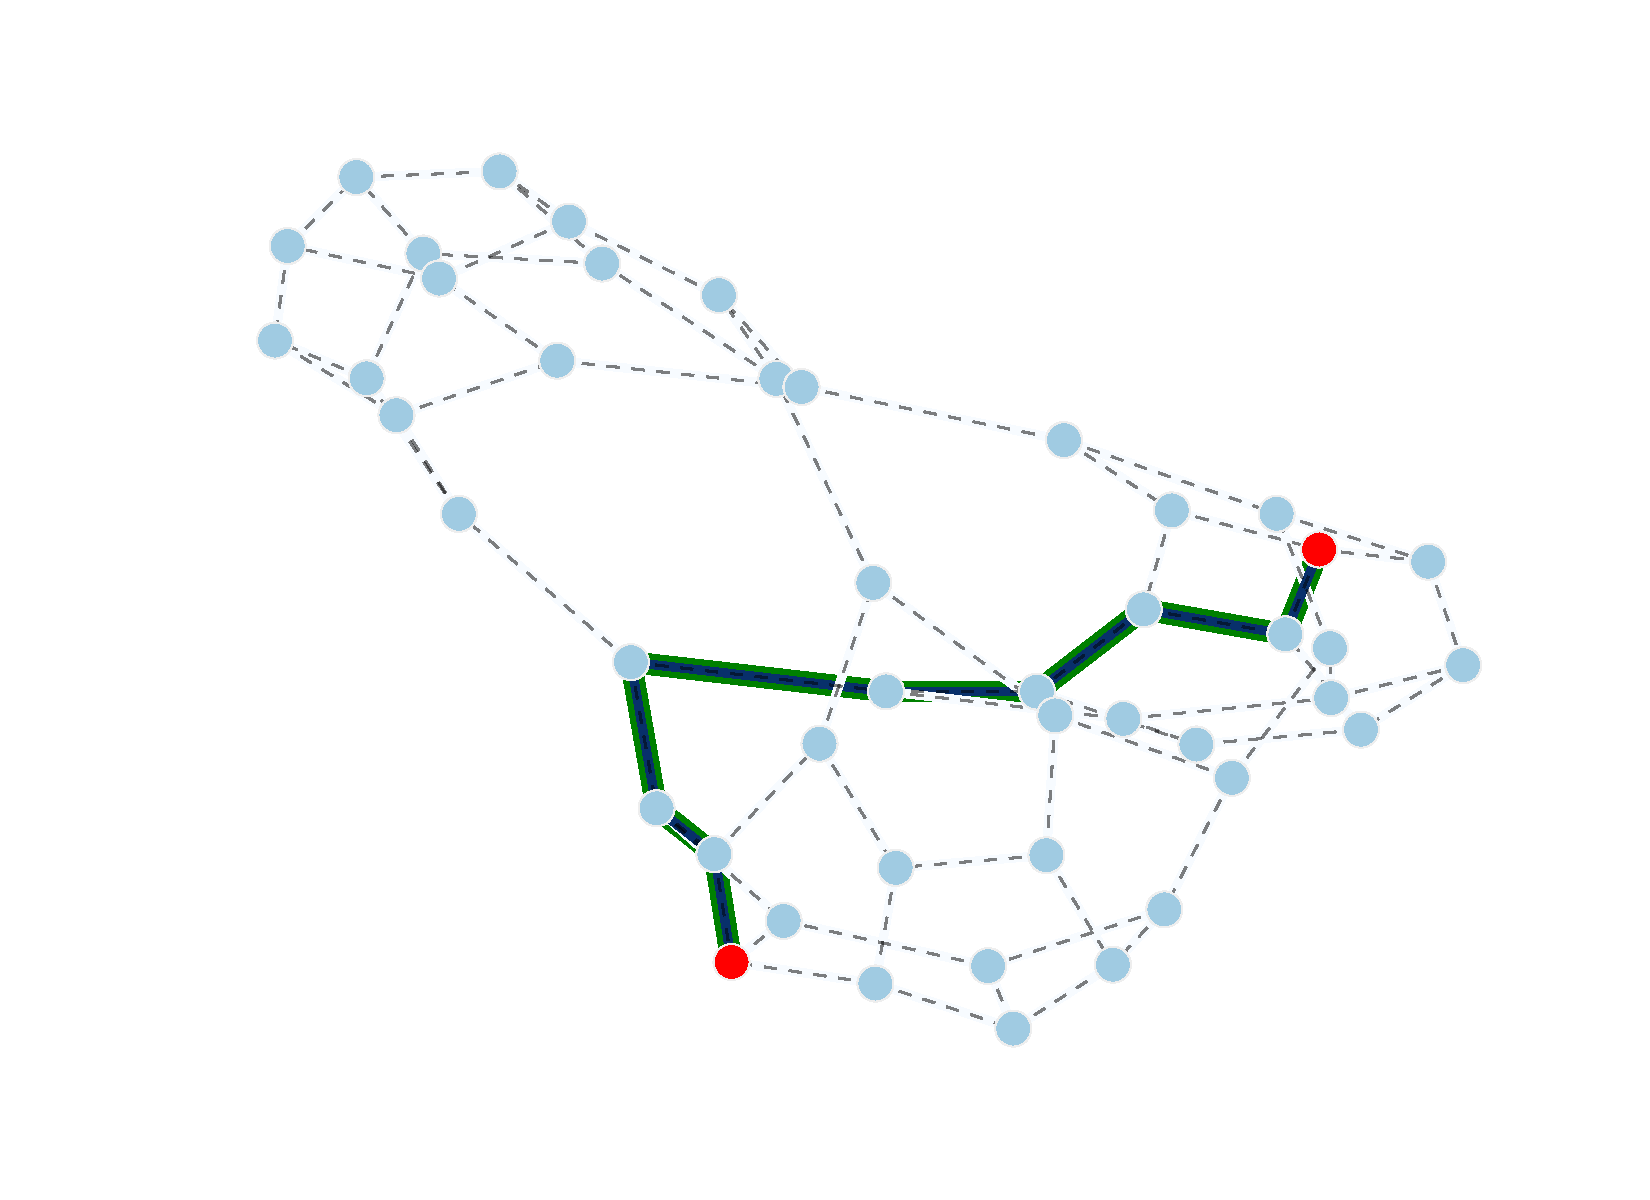
\includegraphics[scale =0.4] {images/section3/pheromones_100_05.pdf}
	\label{fig:figure102}
}
%\caption[Optional caption for list of figures]{Caption of subfigures \subref{fig:subfig1}, \subref{fig:subfig2}}
\label{fig:figure10}
\end{figure}


\newpage
\subsection{Conclusions}
We can conclude that in the first configuration with $\rho = 0.1$ the algorithm are able to remember some paths in order to achieve the best one. The second configuration has a high value to $\rho = 0.5$, therefore, algorithm can discard best solutions growing the exploration factor, however, sometimes can not reach the goal of get the shortest path
\\
\\
We can see that $k=5$ and $k=10$ is not enought to reach the best fitness and therefore to reach the shortest path.
\newpage
\section{Behavior analysis of collective exploration ensemble algorithm}

We perform the anlysis with a different number of robots $ k=\{5,10,50,100\}$

\subsection{$k=5$}

\begin{figure}[ht]
\centering
\subfigure[Fitness evolution]{
	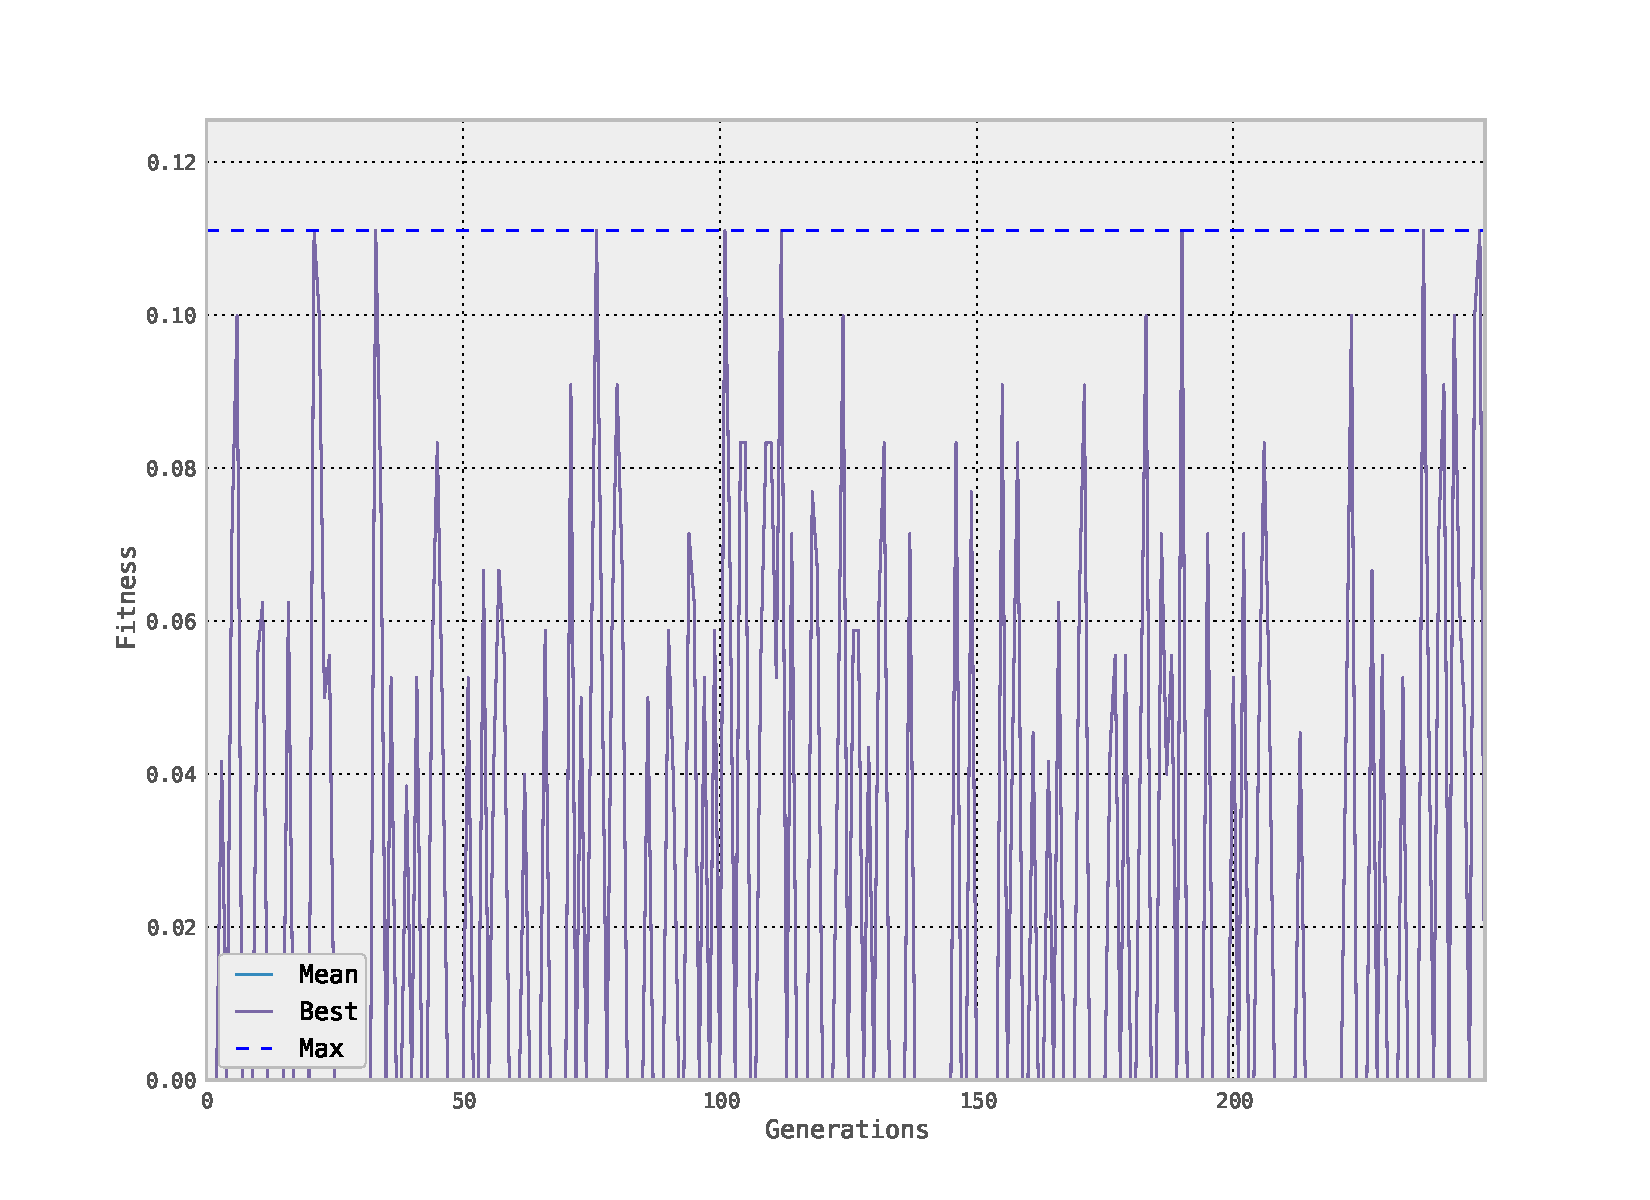
\includegraphics[scale =0.3] {images/section1/fitness_bush_mosteller_update_ProportionalAnt.pdf}
	\label{fig:subfig11}
}
\subfigure[Pheromones per edge]{
	\includegraphics[scale =0.3] {images/section1/pheromones_bush_mosteller_update_ProportionalAnt.pdf}
	\label{fig:subfig12}
}
%\caption[Optional caption for list of figures]{Caption of subfigures \subref{fig:subfig1}, \subref{fig:subfig2}}
\label{fig:fig1}
\end{figure}









\subsection{$k=10$}




\subsection{$k=50$}



\subsection{$k=100$}




\newpage
\subsection{Conclusions}
Conclusions
\newpage
\subsection{Final Conclusions}

Several algorithms has been implemented and tested. We observe that we can identify main parameters like $\rho$ in order to enhance exploration or enhance exploitation. Also, several approachs have been studied in a real problem trough a labeled graph map. 
\\
We provide our source code\footnote{https://github.com/yarox/alos} in order to allow researchs and students check our results and experiment with this algorithms.



\end{document}



